%% LyX 2.4.3 created this file.  For more info, see https://www.lyx.org/.
%% Do not edit unless you really know what you are doing.
\documentclass[journal,article,submit,pdftex,moreauthors]{Definitions/mdpi}
\usepackage{textcomp}
\usepackage[utf8]{inputenc}
\usepackage{color}
\usepackage{array}
\usepackage{longtable}
\usepackage{float}
\usepackage{url}
\usepackage{varwidth}
\usepackage{pdflscape}
\usepackage{amsmath}
\usepackage{graphicx}
\PassOptionsToPackage{normalem}{ulem}
\usepackage{ulem}

\makeatletter

%%%%%%%%%%%%%%%%%%%%%%%%%%%%%% LyX specific LaTeX commands.

\Title{ARQ2: Toward Stability-Aware Hybrid Optimization on Complex and Noisy
Search Problems}

\TitleCitation{ARQ2: Toward Stability-Aware Hybrid Optimization on Complex and Noisy
Search Problems}

\Author{Vasileios Charilogis$^{1}$, Ioannis G. Tsoulos$^{2,*}$ and Anna
Maria Gianni $^{3}$}

\AuthorNames{Vasileios Charilogis, Ioannis G. Tsoulos and Anna Maria Gianni }

\AuthorCitation{Charilogis, V., Tsoulos, I.G., Gianni, A. M.}


\address{$^{1}$\quad{}Department of Informatics and Telecommunications,
University of Ioannina, 47150 Kostaki Artas, Greece, v.charilog@uoi.gr\\
$^{2}$\quad{}Department of Informatics and Telecommunications, University
of Ioannina, 47150 Kostaki Artas, Greece, itsoulos@uoi.gr\\
$^{3}$\quad{}Department of Informatics and Telecommunications, University
of Ioannina, 47150 Kostaki Artas, Greece, am.gianni@uoi.gr}


\corres{Correspondence: itsoulos@uoi.gr}


\abstract{ARQ2 is introduced as a next-generation extension of the ARQ (Archive-guided
Roulette-based with Quarantine) optimization framework, which was
originally established as a cohesive strategy for achieving stable
performance on difficult and noisy search landscapes. While rooted
in the core principles of the original design, ARQ2 advances this
foundation through a more refined integration of adaptive search,
archive-guided exploration, controlled replacement, and robustness-aware
population management. In doing so, it moves beyond the level of a
simple algorithmic modification and emerges as a distinct methodological
development within hybrid continuous optimization. Its significance
lies in shaping a more mature and experimentally substantiated variant
that promotes dependable behavior, consistent search quality, and
balanced exploration-exploitation dynamics across diverse optimization
environments. Empirical evaluation against nine established optimizers
on 36 continuous optimization problems yields an overall average rank
of 1.958, with 25 rank-1 placements and a mean-value improvement over
ARQ on 21 out of 36 problems, confirming the stronger robustness and
repeated-run reliability of the proposed design. As such, ARQ2 contributes
to the ongoing development of stability-oriented optimization methodologies
and reinforces the scientific relevance of this design line in the
contemporary literature.}


\keyword{Continuous Optimization; Hybrid Metaheuristics; Adaptive Search;
Robustness; Stability-Aware Design; Derivative-Free Methods; ARQ Method}

%% Because html converters don't know tabularnewline
\providecommand{\tabularnewline}{\\}
%% Variable width box for table cells
\newenvironment{cellvarwidth}[1][t]
    {\begin{varwidth}[#1]{\linewidth}}
    {\@finalstrut\@arstrutbox\end{varwidth}}
\floatstyle{ruled}
\newfloat{algorithm}{tbp}{loa}
\providecommand{\algorithmname}{Algorithm}
\floatname{algorithm}{\protect\algorithmname}

%%%%%%%%%%%%%%%%%%%%%%%%%%%%%% Textclass specific LaTeX commands.
\newenvironment{lyxlist}[1]
	{\begin{list}{}
		{\settowidth{\labelwidth}{#1}
		 \setlength{\leftmargin}{\labelwidth}
		 \addtolength{\leftmargin}{\labelsep}
		 \renewcommand{\makelabel}[1]{##1\hfil}}}
	{\end{list}}

%%%%%%%%%%%%%%%%%%%%%%%%%%%%%% User specified LaTeX commands.
\usepackage{rotating}

%  LaTeX support: latex@mdpi.com 
%  For support, please attach all files needed for compiling as well as the log file, and specify your operating system, LaTeX version, and LaTeX editor.

%=================================================================


% For posting an early version of this manuscript as a preprint, you may use "preprints" as the journal and change "submit" to "accept". The document class line would be, e.g., \documentclass[preprints,article,accept,moreauthors,pdftex]{mdpi}. This is especially recommended for submission to arXiv, where line numbers should be removed before posting. For preprints.org, the editorial staff will make this change immediately prior to posting.

%--------------------
% Class Options:
%--------------------
%----------
% journal
%----------
% Choose between the following MDPI journals:
% acoustics, actuators, addictions, admsci, adolescents, aerospace, agriculture, agriengineering, agronomy, ai, algorithms, allergies, alloys, analytica, animals, antibiotics, antibodies, antioxidants, applbiosci, appliedchem, appliedmath, applmech, applmicrobiol, applnano, applsci, aquacj, architecture, arts, asc, asi, astronomy, atmosphere, atoms, audiolres, automation, axioms, bacteria, batteries, bdcc, behavsci, beverages, biochem, bioengineering, biologics, biology, biomass, biomechanics, biomed, biomedicines, biomedinformatics, biomimetics, biomolecules, biophysica, biosensors, biotech, birds, bloods, blsf, brainsci, breath, buildings, businesses, cancers, carbon, cardiogenetics, catalysts, cells, ceramics, challenges, chemengineering, chemistry, chemosensors, chemproc, children, chips, cimb, civileng, cleantechnol, climate, clinpract, clockssleep, cmd, coasts, coatings, colloids, colorants, commodities, compounds, computation, computers, condensedmatter, conservation, constrmater, cosmetics, covid, crops, cryptography, crystals, csmf, ctn, curroncol, currophthalmol, cyber, dairy, data, dentistry, dermato, dermatopathology, designs, diabetology, diagnostics, dietetics, digital, disabilities, diseases, diversity, dna, drones, dynamics, earth, ebj, ecologies, econometrics, economies, education, ejihpe, electricity, electrochem, electronicmat, electronics, encyclopedia, endocrines, energies, eng, engproc, ent, entomology, entropy, environments, environsciproc, epidemiologia, epigenomes, est, fermentation, fibers, fintech, fire, fishes, fluids, foods, forecasting, forensicsci, forests, foundations, fractalfract, fuels, futureinternet, futureparasites, futurepharmacol, futurephys, futuretransp, galaxies, games, gases, gastroent, gastrointestdisord, gels, genealogy, genes, geographies, geohazards, geomatics, geosciences, geotechnics, geriatrics, hazardousmatters, healthcare, hearts, hemato, heritage, highthroughput, histories, horticulturae, humanities, humans, hydrobiology, hydrogen, hydrology, hygiene, idr, ijerph, ijfs, ijgi, ijms, ijns, ijtm, ijtpp, immuno, informatics, information, infrastructures, inorganics, insects, instruments, inventions, iot, j, jal, jcdd, jcm, jcp, jcs, jdb, jeta, jfb, jfmk, jimaging, jintelligence, jlpea, jmmp, jmp, jmse, jne, jnt, jof, joitmc, jor, journalmedia, jox, jpm, jrfm, jsan, jtaer, jzbg, kidney, kidneydial, knowledge, land, languages, laws, life, liquids, literature, livers, logics, logistics, lubricants, lymphatics, machines, macromol, magnetism, magnetochemistry, make, marinedrugs, materials, materproc, mathematics, mca, measurements, medicina, medicines, medsci, membranes, merits, metabolites, metals, meteorology, methane, metrology, micro, microarrays, microbiolres, micromachines, microorganisms, microplastics, minerals, mining, modelling, molbank, molecules, mps, msf, mti, muscles, nanoenergyadv, nanomanufacturing, nanomaterials, ncrna, network, neuroglia, neurolint, neurosci, nitrogen, notspecified, nri, nursrep, nutraceuticals, nutrients, obesities, oceans, ohbm, onco, oncopathology, optics, oral, organics, organoids, osteology, oxygen, parasites, parasitologia, particles, pathogens, pathophysiology, pediatrrep, pharmaceuticals, pharmaceutics, pharmacoepidemiology, pharmacy, philosophies, photochem, photonics, phycology, physchem, physics, physiologia, plants, plasma, pollutants, polymers, polysaccharides, poultry, powders, preprints, proceedings, processes, prosthesis, proteomes, psf, psych, psychiatryint, psychoactives, publications, quantumrep, quaternary, qubs, radiation, reactions, recycling, regeneration, religions, remotesensing, reports, reprodmed, resources, rheumato, risks, robotics, ruminants, safety, sci, scipharm, seeds, sensors, separations, sexes, signals, sinusitis, skins, smartcities, sna, societies, socsci, software, soilsystems, solar, solids, sports, standards, stats, stresses, surfaces, surgeries, suschem, sustainability, symmetry, synbio, systems, taxonomy, technologies, telecom, test, textiles, thalassrep, thermo, tomography, tourismhosp, toxics, toxins, transplantology, transportation, traumacare, traumas, tropicalmed, universe, urbansci, uro, vaccines, vehicles, venereology, vetsci, vibration, viruses, vision, waste, water, wem, wevj, wind, women, world, youth, zoonoticdis 

%---------
% article
%---------
% The default type of manuscript is "article", but can be replaced by: 
% abstract, addendum, article, book, bookreview, briefreport, casereport, comment, commentary, communication, conferenceproceedings, correction, conferencereport, entry, expressionofconcern, extendedabstract, datadescriptor, editorial, essay, erratum, hypothesis, interestingimage, obituary, opinion, projectreport, reply, retraction, review, perspective, protocol, shortnote, studyprotocol, systematicreview, supfile, technicalnote, viewpoint, guidelines, registeredreport, tutorial
% supfile = supplementary materials

%----------
% submit
%----------
% The class option "submit" will be changed to "accept" by the Editorial Office when the paper is accepted. This will only make changes to the frontpage (e.g., the logo of the journal will get visible), the headings, and the copyright information. Also, line numbering will be removed. Journal info and pagination for accepted papers will also be assigned by the Editorial Office.

%------------------
% moreauthors
%------------------
% If there is only one author the class option oneauthor should be used. Otherwise use the class option moreauthors.

%---------
% pdftex
%---------
% The option pdftex is for use with pdfLaTeX. If eps figures are used, remove the option pdftex and use LaTeX and dvi2pdf.

%=================================================================
% MDPI internal commands - do not modify
\firstpage{1} 
 
\setcounter{page}{\@firstpage} 

\pubvolume{1}
\issuenum{1}
\articlenumber{0}
\pubyear{2024}
\copyrightyear{2024}
%\externaleditor{Academic Editor: Firstname Lastname} % For journal Automation, please change Academic Editor to "Communicated by"
\datereceived{}
\daterevised{ } % Comment out if no revised date
\dateaccepted{}
\datepublished{}
%\datecorrected{} % Corrected papers include a "Corrected: XXX" date in the original paper.
%\dateretracted{} % Corrected papers include a "Retracted: XXX" date in the original paper.
\hreflink{} % If needed use \linebreak
%\doinum{}
%------------------------------------------------------------------
% The following line should be uncommented if the LaTeX file is uploaded to arXiv.org
%\pdfoutput=1

%=================================================================
% Add packages and commands here. The following packages are loaded in our class file: fontenc, inputenc, calc, indentfirst, fancyhdr, graphicx, epstopdf, lastpage, ifthen, lineno, float, amsmath, setspace, enumitem, mathpazo, booktabs, titlesec, etoolbox, tabto, xcolor, soul, multirow, microtype, tikz, totcount, changepage, attrib, upgreek, cleveref, amsthm, hyphenat, natbib, hyperref, footmisc, url, geometry, newfloat, caption

%=================================================================
%% Please use the following mathematics environments: Theorem, Lemma, Corollary, Proposition, Characterization, Property, Problem, Example, ExamplesandDefinitions, Hypothesis, Remark, Definition, Notation, Assumption
%% For proofs, please use the proof environment (the amsthm package is loaded by the MDPI class).

%=================================================================
% The fields PACS, MSC, and JEL may be left empty or commented out if not applicable
%\PACS{J0101}
%\MSC{}
%\JEL{}

%%%%%%%%%%%%%%%%%%%%%%%%%%%%%%%%%%%%%%%%%%
% Only for the journal Diversity
%\LSID{\url{http://}}

%%%%%%%%%%%%%%%%%%%%%%%%%%%%%%%%%%%%%%%%%%
% Only for the journal Applied Sciences:
%\featuredapplication{Authors are encouraged to provide a concise description of the specific application or a potential application of the work. This section is not mandatory.}
%%%%%%%%%%%%%%%%%%%%%%%%%%%%%%%%%%%%%%%%%%

%%%%%%%%%%%%%%%%%%%%%%%%%%%%%%%%%%%%%%%%%%
% Only for the journal Data:
%\dataset{DOI number or link to the deposited data set in cases where the data set is published or set to be published separately. If the data set is submitted and will be published as a supplement to this paper in the journal Data, this field will be filled by the editors of the journal. In this case, please make sure to submit the data set as a supplement when entering your manuscript into our manuscript editorial system.}

%\datasetlicense{license under which the data set is made available (CC0, CC-BY, CC-BY-SA, CC-BY-NC, etc.)}

%%%%%%%%%%%%%%%%%%%%%%%%%%%%%%%%%%%%%%%%%%
% Only for the journal Toxins
%\keycontribution{The breakthroughs or highlights of the manuscript. Authors can write one or two sentences to describe the most important part of the paper.}

%%%%%%%%%%%%%%%%%%%%%%%%%%%%%%%%%%%%%%%%%%
% Only for the journal Encyclopedia
%\encyclopediadef{Instead of the abstract}
%\entrylink{The Link to this entry published on the encyclopedia platform.}
%%%%%%%%%%%%%%%%%%%%%%%%%%%%%%%%%%%%%%%%%%

%%%%%%%%%%%%%%%%%%%%%%%%%%%%%%%%%%%%%%%%%%
% Only for the journal Advances in Respiratory Medicine
%\addhighlights{yes}
%\renewcommand{\addhighlights}{%

%\noindent This is an obligatory section in “Advances in Respiratory Medicine”, whose goal is to increase the discoverability and readability of the article via search engines and other scholars. Highlights should not be a copy of the abstract, but a simple text allowing the reader to quickly and simplified find out what the article is about and what can be cited from it. Each of these parts should be devoted up to 2~bullet points.\vspace{3pt}\\
%\textbf{What are the main findings?}
% \begin{itemize}[labelsep=2.5mm,topsep=-3pt]
% \item First bullet.
% \item Second bullet.
% \end{itemize}\vspace{3pt}
%\textbf{What is the implication of the main finding?}
% \begin{itemize}[labelsep=2.5mm,topsep=-3pt]
% \item First bullet.
% \item Second bullet.
% \end{itemize}
%}
%%%%%%%%%%%%%%%%%%%%%%%%%%%%%%%%%%%%%%%%%%
% Added by lyx2lyx
\usepackage{array}
\usepackage[noend]{algpseudocode}
\algrenewcommand\algorithmicindent{1.0em}

\ifdefined\showcaptionsetup
 % Caption package is used. Advise subfig not to load it again.
 \PassOptionsToPackage{caption=false}{subfig}
\fi
\usepackage{subfig}
\makeatother

\begin{document}
\maketitle

\section{Introduction}

This study considers continuous black-box minimization over a bounded
hyper-rectangular domain, where only pointwise evaluations of the
objective function are assumed to be available and derivative information
may be unavailable. In constrained settings, the search is restricted
to the feasible subset of the bounded domain, while bound violations
may be repaired through projection and more general constraint violations
may be absorbed through penalty-based formulations. This viewpoint
is standard in derivative-free and constrained optimization, especially
when the objective function is nonlinear, multimodal, noisy, or computationally
expensive \citep{Rios}, \citep{Coello}.

\begin{equation}
\min_{\mathbf{x}\in\Omega}\,f(\mathbf{x}),\qquad\Omega=\prod_{j=1}^{n}[l_{j},u_{j}]\subset\mathbb{R}^{n}
\end{equation}

Given an evaluation budget $N$, an optimizer produces candidate points
$\mathbf{x}^{(1)},\mathbf{x}^{(2)},\ldots,\mathbf{x}^{(N)}$ and tracks
the best-so-far objective value defined by

\begin{equation}
f^{\star}(m)=\min_{1\leq\tau\leq m}\,f\bigl(\mathbf{x}^{(\tau)}\bigr)
\end{equation}

Over $R$ independent runs, terminal performance is summarized by

\begin{equation}
\mathrm{Best}=\min_{1\leq r\leq R}f_{r}^{\star}(N),\qquad\mathrm{Mean}=\frac{1}{R}\sum_{r=1}^{R}f_{r}^{\star}(N)
\end{equation}

This compact formulation is sufficient for benchmarking derivative-free
optimizers under a fixed computational budget and for comparing their
terminal effectiveness across repeated runs \citep{Rios}.

The modern optimization literature contains a wide spectrum of algorithmic
paradigms developed for hard nonlinear and black-box search problems.
Representative examples include simulated annealing \citep{Kirkpatrick},
particle swarm optimization \citep{Kennedy}, covariance matrix adaptation
evolution strategy \citep{Hansen}, ant system \citep{Dorigo}, tabu
search \citep{Glover}, scatter search \citep{Glover2}, harmony search
\citep{Geem}, artificial bee colony \citep{Karaboga}, firefly algorithm
\citep{Yang}, cuckoo search \citep{Yang2}, bat algorithm \citep{Yang3},
teaching-learning-based optimization \citep{Rao}, gravitational search
algorithm \citep{Rashedi}, grey wolf optimizer \citep{Mirjalili},
whale optimization algorithm \citep{Mirjalili2}, biogeography-based
optimization \citep{Simon}, invasive weed optimization \citep{Mehrabian},
shuffled frog-leaping algorithm \citep{Eusuff}, memetic algorithms
\citep{Krasnogor}, and estimation of distribution algorithms \citep{Larra=0000F1aga}.

This methodological diversity highlights a central feature of continuous
optimization: no single search mechanism is uniformly reliable across
all problem classes, and practical performance depends strongly on
how exploration, exploitation, adaptation, and population diversity
are coordinated. As a result, contemporary research has increasingly
emphasized robust search behavior, parameter control, and strategy
adaptation rather than purely static algorithmic designs \citep{Rios},
\citep{Krasnogor}, \citep{Larra=0000F1aga}. 

Within this broad landscape, Differential Evolution (DE) has become
one of the most influential frameworks for real-parameter optimization
\citep{Storn}, \citep{Ahmad}, \citep{Das}. Its compact algorithmic
structure can induce markedly different search behaviors through the
choice of mutation base vector, difference scheme, and crossover operator.
Classical strategies range from the exploratory DE/rand/1/bin, which
uses a randomly selected base vector and promotes diversity, to the
exploitative DE/best/1/bin, which perturbs the incumbent solution
and accelerates local convergence at the risk of premature convergence
\citep{Storn}, \citep{Ahmad}, \citep{Das}. Intermediate schemes
such as DE/current-to-best/1/bin balance these tendencies by simultaneously
attracting each individual toward the best solution and injecting
a differential perturbation term \citep{Storn}, \citep{Das}. The
most influential modern realization of this principle is DE/current-to-pbest/1/bin,
popularized by JADE \citep{Zhang}, which replaces the unique best
individual with a solution drawn from the top p\% of the population
and extends the difference vector to include an external archive,
thereby combining directed elite guidance with historical diversity.
The suffix /bin denotes binomial crossover, where each coordinate
is updated independently, in contrast to /exp crossover, which updates
a contiguous block \citep{Storn}, \citep{Das}. The same strategic
sensitivity applies to the control parameters F and CR, motivating
a large body of work on self-adaptation, strategy adaptation, archive
usage, and success-history based parameter control, with representative
milestones including jDE \citep{Brest}, SaDE \citep{Qin}, JADE,
CoDE \citep{Wang}, SHADE \citep{Wang2}, and L-SHADE \citep{Tanabe}.
Taken together, these developments established that the effectiveness
of DE depends on the coordinated interaction of mutation strategy,
crossover policy, parameter memories, archive usage, and population
management, providing the conceptual basis from which modern hybrid,
adaptive, and stability-oriented optimizers are constructed \citep{Ahmad,Brest,Qin,Zhang,Wang,Wang2,Tanabe,Das}. 

The empirical study further situates the proposed ARQ2 against a heterogeneous
set of established and recent optimizers, namely its predecessor ARQ
\citep{Charilogis}, the cooperative ensemble EA4Eig \citep{Bujok},
\citep{Biedrzycki}, the competition-oriented jSO \citep{Brest2},
the classical self-adaptive DE variant jDE \citep{Brest3}, the recent
multi-operator mLSHADE-RL \citep{Chauhan}, the swarm-based CLPSO
\citep{Liang}, the hybrid DE framework TRIDENT-DE \citep{Charilogis2},
the constrained-optimization-oriented UDE-III \citep{Trivedi}, and
the strategy-adaptive SaDE \citep{Qin}. This selection was designed
to cover multiple search philosophies, including success-history adaptation,
self-adaptation, strategy adaptation, cooperative and ensemble search,
archive-assisted differential evolution, swarm intelligence, and hybrid
restart mechanisms, thereby avoiding a comparison restricted to a
single algorithmic family.

Several of these competitors are also closely connected to the IEEE
Congress on Evolutionary Computation (CEC) ecosystem. jSO \citep{Brest2}
was introduced in the context of the CEC 2017 single-objective real-parameter
optimization track, EA4Eig \citep{Bujok}, \citep{Biedrzycki} originates
from the cooperative model proposed for the CEC 2022 single-objective
numerical optimization setting and was later analyzed as the winner
of that competition, mLSHADE-RL \citep{Chauhan} was proposed for
the CEC 2024 single-objective bound-constrained competition while
explicitly extending LSHADE-cnEpSin, one of the winning lines from
CEC 2017, and UDE-III \citep{Trivedi} was developed for the CEC 2024
constrained real-parameter competition while building on IUDE/UDE-II,
which achieved first rank in the CEC 2018 constrained-optimization
competition. By contrast, jDE \citep{Brest3}, SaDE \citep{Qin2},
and CLPSO \citep{Liang} serve as canonical literature baselines,
whereas ARQ \citep{Charilogis} and TRIDENT-DE \citep{Charilogis2}
represent recent methodological baselines from the broader optimization
literature rather than direct competition submissions.

This competition-aware choice of baselines is further consistent with
the benchmark culture documented by the Al-Roomi repository \citep{Al-Roomi},
which curates IEEE CEC databases and disseminates collections including
the CEC 2011 real-world optimization suite as well as later real-parameter
and constrained benchmark tracks. Consequently, the present study
is positioned not only against widely cited standalone optimizers,
but also against methods shaped by the evaluation practices of modern
CEC benchmark campaigns. 

Overall, the preceding discussion highlights that modern continuous
optimization is shaped not only by the quality of individual search
operators, but also by the way mutation strategies, parameter adaptation,
archive usage, population management, and robustness mechanisms are
combined into a coherent search design. Although the literature offers
a rich set of competitive optimizers, including several methods associated
with CEC benchmark campaigns, their behavior remains problem-dependent
and no single scheme can be assumed to provide uniformly stable performance
across heterogeneous search landscapes. This observation motivates
the development of new optimization designs that place greater emphasis
on consistency, controlled search dynamics, and robustness under demanding
conditions. Against this background, it is worth clarifying how ARQ2
specifically addresses noisy and multimodal search landscapes. With
respect to noisy environments, three complementary mechanisms reduce
the distorting influence of stochastic fitness perturbations: the
quarantine stage suppresses noise-inflated solutions by relocating
outliers around the centroid of the better half of the population,
the restricted tournament replacement prevents fortuitous noise-driven
improvements from displacing well-positioned individuals, and the
success-history adaptation accumulates evidence from genuinely successful
trials across multiple iterations, making parameter estimates less
susceptible to isolated noisy outcomes. With respect to multimodal
landscapes, the IDE branch contributes a structurally distinct search
dynamic that reduces concentration around a single attractor, the
roulette-based scheduler dynamically reallocates resources between
branches based on observed credit histories, and the progress-dependent
attraction coefficient $K(\pi)$ provides a principled transition
from broader exploration in early stages to focused refinement in
later stages, a property that is particularly beneficial in landscapes
with multiple competing local optima.

Against this background, the principal contributions of the present
study can be summarized as follows. First, ARQ2 introduces an asymmetric
hybrid architecture in which two internal search branches, ARQ and
IDE, operate on a shared population and a shared external archive,
while the quarantine and micro-restart stabilization mechanisms remain
attached exclusively to the ARQ side, preserving the corrective role
of the original design without duplicating its machinery in the auxiliary
branch. Second, an endogenous roulette-based branch scheduler is proposed,
which dynamically reallocates computational resources between branches
based on observed credit histories and prevents permanent dominance
through a principled credit-reset mechanism. Third, a bootstrap phase
is introduced to stabilize early credit statistics before competitive
branch selection begins. Fourth, the ARQ-side mutation rule is enriched
by a progress-dependent attraction coefficient $K(\pi)$ that modulates
elite guidance as a function of the optimization progress ratio, making
the inherited search dynamic more flexible within the hybrid environment.
Collectively, these contributions define ARQ2 as an integrated hybrid
architecture rather than a straightforward combination of existing
components.

The remainder of the article is organized as follows. Section \ref{sec:ARQ2}
presents the design overview of ARQ2 and its relation to ARQ (Section
\ref{subsec:DesignOverviewRelation}), followed by the overall workflow
and roulette-based scheduling mechanism (Section \ref{subsec:workflow}).
Section \ref{sec:experiments} describes the experimental configuration
and reproducibility protocol (Section \ref{subsec:generalsettings})
and the benchmark testbed, covering real-world (Section \ref{realworldfunctions})
and classical non-realworld problems (Section \ref{nonrealworldfunctions}).
Section \ref{sec:results} presents the comparative results, including
overall rankings and statistical significance analysis, followed by
empirical convergence complexity and runtime overhead (Section \ref{subsec:complexity}),
parameter sensitivity analysis (Section \ref{subsec:sensitivity}),
and strengths and weaknesses of the proposed method (Section \ref{subsec:strengthsWeaknesses}).
Section \ref{sec:conclusions} summarizes the principal findings and
concluding remarks.

\section{ARQ2: A Roulette-Guided Hybrid Extension of ARQ\label{sec:ARQ2}}

\subsection{Design Overview and Relation to ARQ\label{subsec:DesignOverviewRelation}}

ARQ2 is introduced as a hybrid extension of the previously published
ARQ framework rather than as a minor operator-level modification.
The original ARQ was designed as a cohesive optimization scheme that
combines archive-assisted pbest differential evolution, success-history
parameter adaptation, restricted tournament replacement, and an event-driven
stabilization mechanism based on quarantine and targeted micro-restarts.
Since these core components have already been presented in detail
in the original ARQ study, they are not repeated here exhaustively.
Instead, the present section focuses on the architectural modifications
through which ARQ2 extends that design line. \citep{Charilogis}

The central idea behind ARQ2 is to preserve the stability-oriented
backbone of ARQ while embedding a second internal search branch derived
from IDE within the same optimization process. In contrast to ARQ,
which evolves the population through a single cohesive update cycle,
ARQ2 operates through a controller-driven hybrid structure in which
two internal heuristics, namely an ARQ branch and an IDE branch, act
on a shared population and a shared external archive. The method explicitly
implements this hybrid identity at the design level, as reflected
by its own definition as an “ARQ/IDE roulette” scheme with quarantine,
ARQ-only micro-restart, and a jSO-style attraction coefficient. This
already indicates that the proposed method should be interpreted not
as a reformulation of ARQ, but as a broader search architecture built
upon it. \citep{Charilogis}, \citep{Brest2}

More specifically, ARQ2 retains from ARQ the archive-based search
memory, the success-history adaptation of F and CR, the neighborhood-aware
RTR replacement logic, and the robustness-oriented maintenance philosophy.
However, it augments this inherited core in four important ways. First,
it introduces an IDE-based branch with its own search dynamics and
per-individual parameter memories. Second, it employs a roulette-guided
branch scheduler that dynamically decides which internal heuristic
will be activated at each iteration. Third, it includes an early bootstrap
phase that temporarily favors the ARQ branch before the branch-selection
statistics become informative. Fourth, the ARQ-side trial construction
is enriched by a jSO-style coefficient K, which modulates the attraction
toward elite exemplars and makes the inherited ARQ mutation rule more
flexible inside the hybrid environment. These additions collectively
define the methodological identity of ARQ2. \citep{Mirjalili2}, \citep{Charilogis},
\citep{Bujok}, \citep{Brest2}

An equally important aspect of the design is that the hybridization
remains intentionally asymmetric. Although ARQ2 contains two internal
branches, the quarantine mechanism and the targeted micro-restart
remain attached only to the ARQ side. This choice is not incidental,
rather, it preserves the corrective and regenerative role that distinguished
ARQ in the first place, while allowing the IDE branch to contribute
behavioral diversity without duplicating the same stabilization machinery.
In addition, the two branches are not fully isolated from one another,
since they operate on shared population state and archive memory,
while ARQ-side events may also trigger IDE-parameter inheritance or
reset actions. Consequently, ARQ2 is better characterized as an integrated
hybrid architecture than as a simple portfolio of independently running
optimizers. \citep{Charilogis}

From this perspective, the contribution of ARQ2 lies less in the invention
of a single new search operator and more in the coordinated redesign
of the optimization workflow. The method extends ARQ by combining
a stability-aware DE backbone with an auxiliary IDE search regime,
an endogenous heuristic-selection controller, and asymmetric maintenance
mechanisms that preserve robustness while broadening the search behavior.
For this reason, the proposed method is presented in the following
subsections primarily through its workflow and architectural interactions,
rather than through a full rederivation of the already published ARQ
components. \citep{Charilogis}

\subsection{Overall Workflow and Roulette-Based Hybrid Scheduling\label{subsec:workflow}}

ARQ2 evolves a single population under a hybrid controller that activates
one of two internal search branches at each iteration. Let $X=\{x_{i}\}_{i=1}^{N}$
denote the current population, let $A$ denote the external archive,
and let $(x^{\ast},f^{\ast})$ denote the incumbent best solution
and its objective value. Instead of relying on a single homogeneous
update rule, the method follows a controller-driven workflow in which
archive maintenance, branch scheduling, branch execution, branch-dependent
stabilization, and stopping checks are performed in a fixed sequence.
The overall workflow, the roulette-based scheduler, and the IDE-side
routine are therefore presented separately in Figures \ref{fig:mainWorkflow},
\ref{fig:rouletteBasedScheduling}, and \ref{fig:ide}, and in Algorithms
\ref{alg:mainworkflow}, \ref{alg:roulette}, and \ref{alg:ide},
respectively.

\begin{figure}[H]
\centering
\begin{centering}
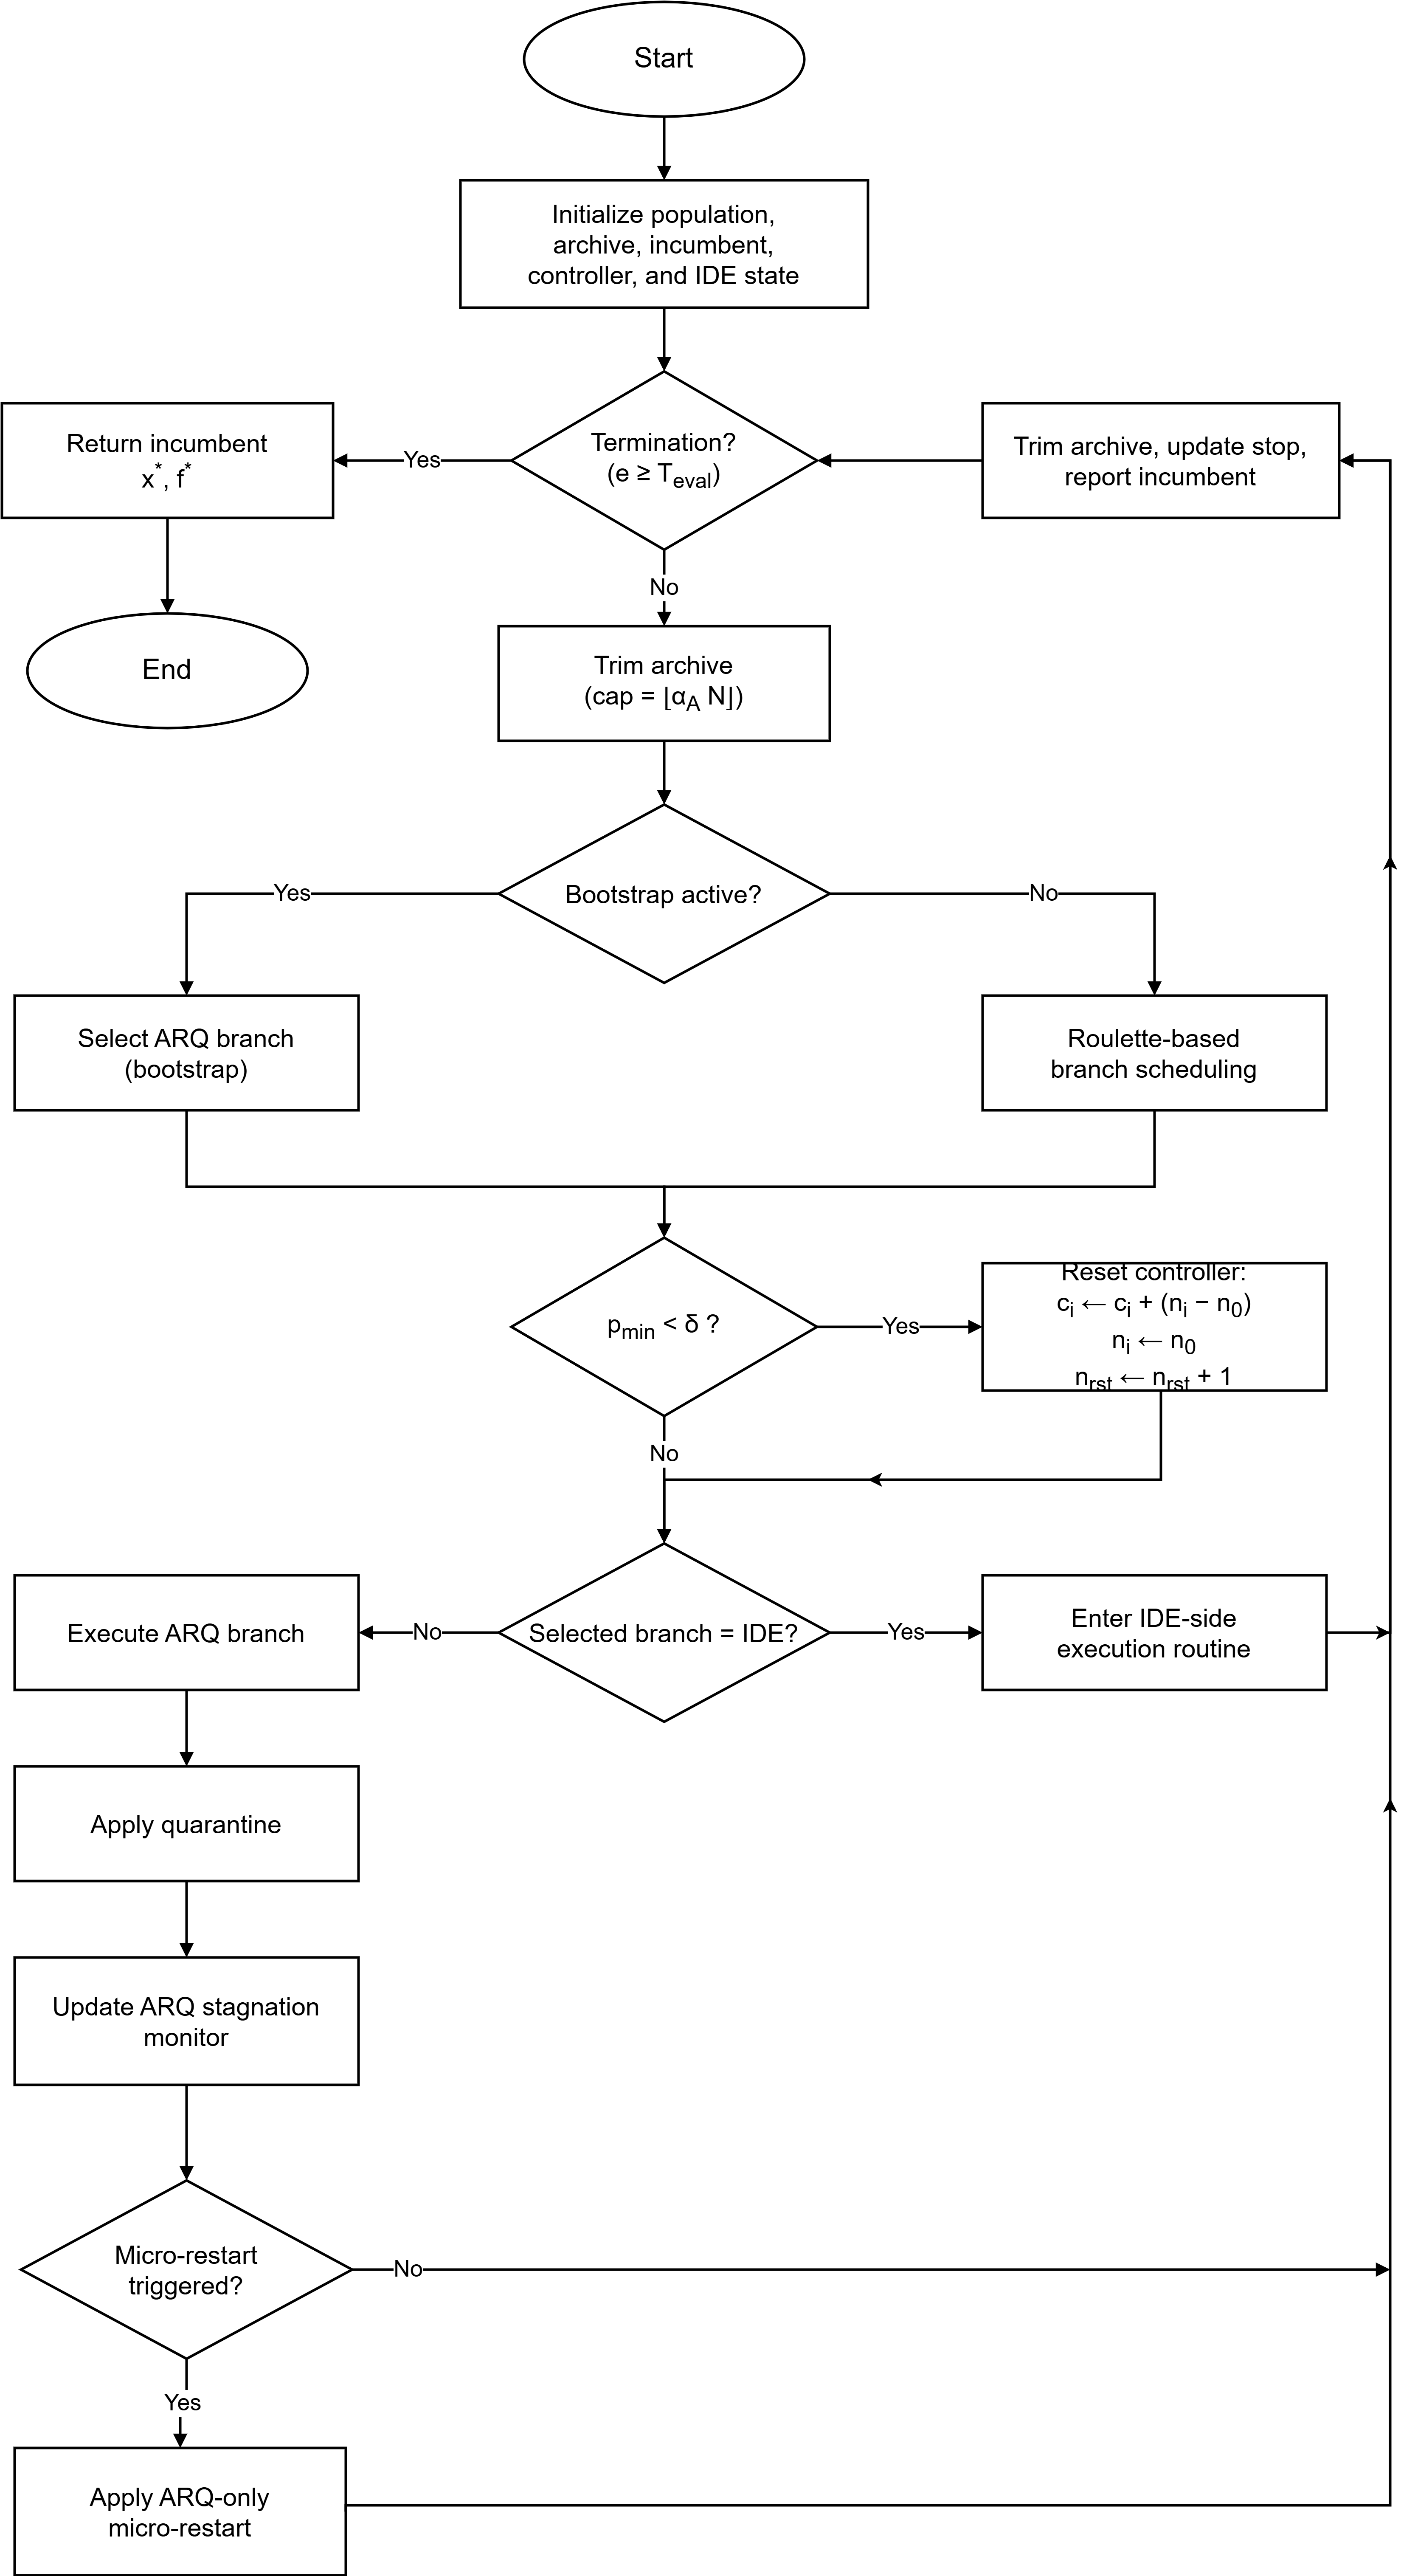
\includegraphics[scale=0.4]{arq2_overall_flow}
\par\end{centering}
\caption{Overall Workflow of ARQ2\label{fig:mainWorkflow}}
\end{figure}

\begin{algorithm}
INPUT

- $f$: objective function

- $\Omega$: box-constrained search domain

- $N$: population size

- $T_{\mathrm{eval}}$: maximum number of function evaluations

- $p$: elite fraction in the ARQ branch

- $\xi$: update fraction in the ARQ branch

- $\mu_{F},\ \mu_{CR}$: ARQ parameter means

- $\alpha_{A}$: archive-rate coefficient

- $\alpha_{o},\ \rho_{o},\ \sigma_{q}$: quarantine parameters

- $\rho_{w},\ \sigma_{r},\ \tau$: ARQ micro-restart parameters

- $h,\ n_{0},\ \delta,\ b$: scheduler parameters

- $\pi_{t},\ \lambda$: IDE phase-threshold and patience parameters

OUTPUT

- $x^{\ast},\ f^{\ast}$

INITIALIZATION

- Initialize population $X=\{x_{i}\}_{i=1}^{N}\subset\Omega$ and
evaluate all individuals

- Set archive $A\leftarrow\varnothing$

- Identify the incumbent best pair $(x^{\ast},f^{\ast})$

- Set $f^{\mathrm{prev}}\leftarrow f^{\ast}$ and $s\leftarrow0$

- Set $n_{i}\leftarrow n_{0}$ and $c_{i}\leftarrow0$ for $i=1,\ldots,h$

- Set $n_{\mathrm{rst}}\leftarrow0$

- Set $e\leftarrow N$

- Initialize the bootstrap counter $b$, the IDE phase threshold $\pi_{t}$,
the patience window $\lambda$, the counter $\lambda_{c}\leftarrow0$,
and the individual IDE memories $\{F_{i}^{\mathrm{IDE}},CR_{i}^{\mathrm{IDE}}\}_{i=1}^{N}$

ARQ2 main pseudocode

01 While $e<T_{\mathrm{eval}}$ do

02 {\scriptsize\hspace{0.5cm}}Trim $A$ to size $\lfloor\alpha_{A}N\rfloor$

03 {\scriptsize\hspace{0.5cm}}Obtain the selected branch and the
updated scheduler state from Algorithm \ref{alg:roulette}

04 {\scriptsize\hspace{0.5cm}}If the IDE branch is selected then

05 {\scriptsize\hspace{0.5cm}\hspace{0.5cm}}Apply the IDE branch
update according to Algorithm \ref{alg:ide}

06 {\scriptsize\hspace{0.5cm}}Else

07 {\scriptsize\hspace{0.5cm}\hspace{0.5cm}}Apply the ARQ branch
update to $X$ and $A$

08 {\scriptsize\hspace{0.5cm}\hspace{0.5cm}}Apply quarantine-based
correction using $\alpha_{o},\ \rho_{o},\ \sigma_{q}$

09 {\scriptsize\hspace{0.5cm}\hspace{0.5cm}}If $f^{\ast}<f^{\mathrm{prev}}$
then

10 {\scriptsize\hspace{0.5cm}\hspace{0.5cm}\hspace{0.5cm}}Set $f^{\mathrm{prev}}\leftarrow f^{\ast}$

11 {\scriptsize\hspace{0.5cm}\hspace{0.5cm}\hspace{0.5cm}}Set $s\leftarrow0$

12 {\scriptsize\hspace{0.5cm}\hspace{0.5cm}}Else

13 {\scriptsize\hspace{0.5cm}\hspace{0.5cm}\hspace{0.5cm}}Set $s\leftarrow s+1$

14 {\scriptsize\hspace{0.5cm}\hspace{0.5cm}}Endif

15 {\scriptsize\hspace{0.5cm}\hspace{0.5cm}}If $s\geq\tau$ then

16 {\scriptsize\hspace{0.5cm}\hspace{0.5cm}\hspace{0.5cm}}Apply
ARQ-only micro-restart to the $\lfloor\rho_{w}N\rfloor$ worst individuals
around $x^{\ast}$

17 {\scriptsize\hspace{0.5cm}\hspace{0.5cm}\hspace{0.5cm}}Set $s\leftarrow0$

18 {\scriptsize\hspace{0.5cm}\hspace{0.5cm}}Endif

19 {\scriptsize\hspace{0.5cm}}Endif

20 {\scriptsize\hspace{0.5cm}}Trim $A$ again to size $\lfloor\alpha_{A}N\rfloor$

21 {\scriptsize\hspace{0.5cm}}Update the stopping state and report
the current incumbent

22 {\scriptsize\hspace{0.5cm}}Set $e$ equal to the current number
of function evaluations

23 Endwhile

24 Return $x^{\ast},\ f^{\ast}$

\caption{Main workflow of ARQ2\label{alg:mainworkflow}}

\end{algorithm}

At initialization, the method evaluates the initial population, constructs
the archive, and identifies the initial incumbent. It also initializes
a stagnation monitor through a reference best value $f^{\mathrm{prev}}$
and a non-improvement counter $s$. The branch scheduler is configured
for $h=2$ competing branches, corresponding to ARQ and IDE. A baseline
branch credit $n_{0}$ is assigned to each branch, the reset threshold
is set to $\delta=1/(5h)$, the initial active credits satisfy $n_{i}=n_{0}$
for $i=1,2$, the cumulative credit-memory terms satisfy $c_{i}=0$,
and the reset counter is initialized as $n_{\mathrm{rst}}=0$. In
addition, a bootstrap counter $b$ is used to enforce the ARQ branch
during the first scheduled iterations. To maintain a common notion
of search progress across the two branches, the algorithm uses the
evaluation-based progress ratio. The value $\delta=1/(5h)$ was selected
to ensure that a reset is triggered before any branch is reduced to
near-zero selection probability, while remaining tolerant enough to
allow meaningful credit differentiation between branches. For $h=2$,
this yields $\delta=0.1$, meaning a reset occurs when one branch
holds less than ten percent of the total selection probability.

\[
\pi=\frac{e}{T_{\mathrm{eval}}},
\]

where $e$ denotes the number of consumed function evaluations and
$T_{\mathrm{eval}}$ denotes the total evaluation budget.

At the beginning of each iteration, the archive is first trimmed so
that its capacity does not exceed

\[
\lfloor\alpha_{A}N\rfloor,
\]

where $\alpha_{A}$ is the archive-size coefficient. The controller
then determines which branch will be executed. If $b>0$, the ARQ
branch is selected deterministically and the bootstrap counter is
decreased by one. This is the only stage in which ARQ has strict priority.
After the bootstrap stage has ended, neither ARQ nor IDE has permanent
priority, instead, both branches compete under the same credit-based
scheduler.

\begin{figure}[H]
\centering
\begin{centering}
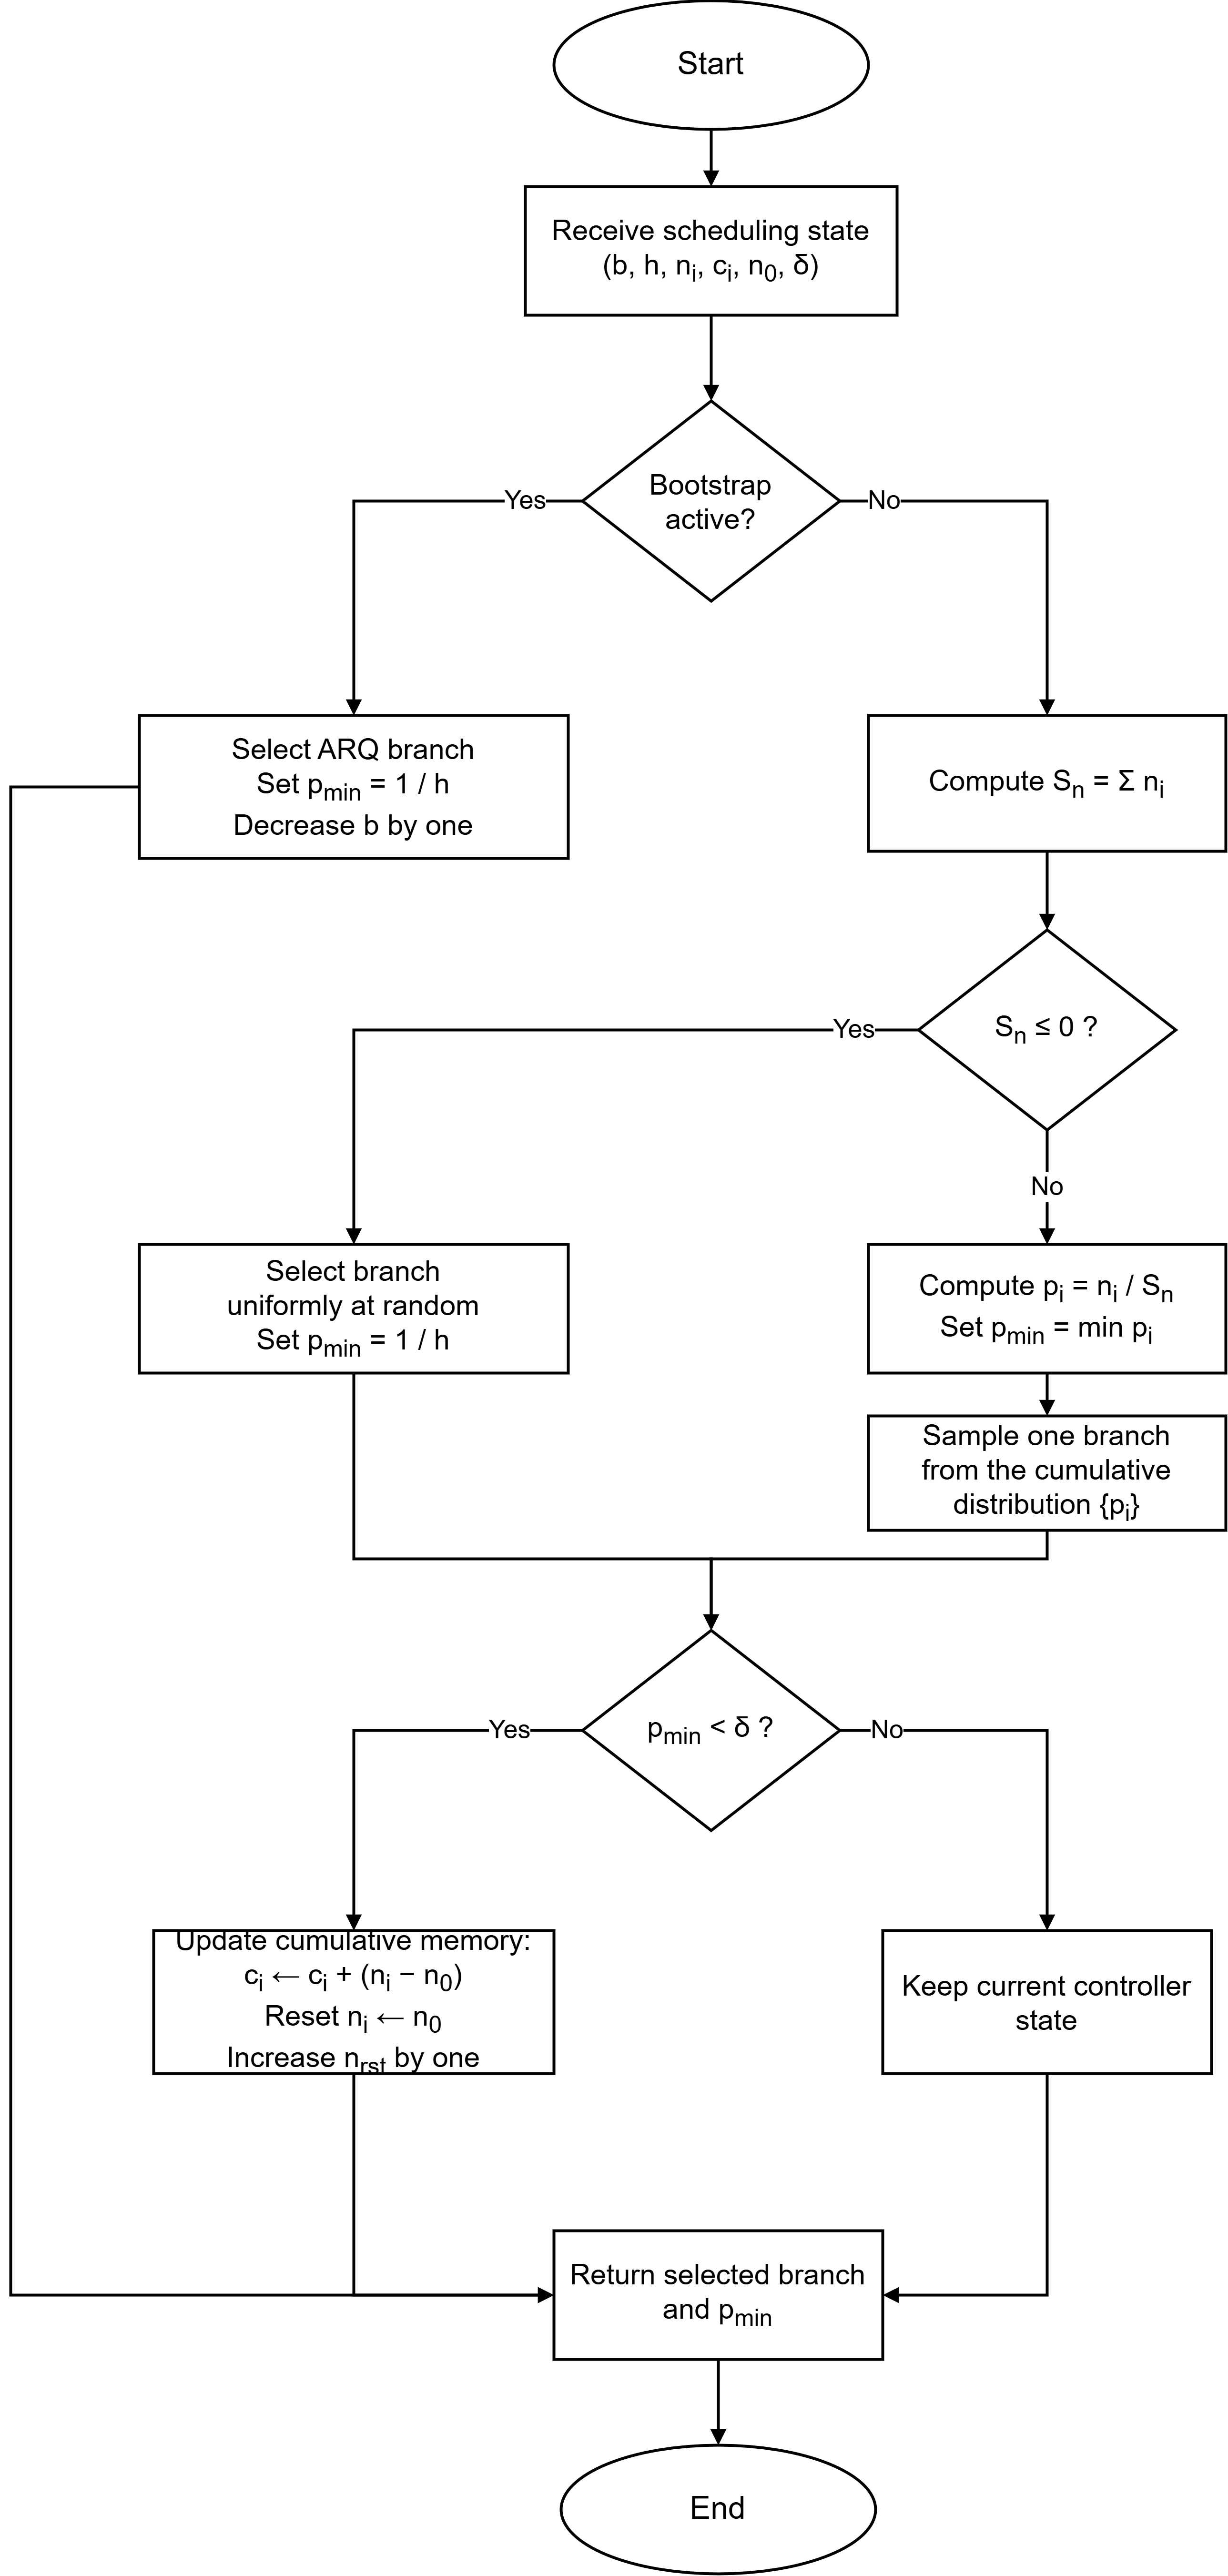
\includegraphics[scale=0.4]{arq2_roulette_flow}
\par\end{centering}
\caption{Roulette-Based Branch Scheduling in ARQ2\label{fig:rouletteBasedScheduling}}
\end{figure}

\begin{algorithm}
INPUT

- $h$: number of internal search branches

- $n_{0}$: baseline branch credit

- $\delta$: reset threshold

- $b$: bootstrap counter

- $\{n_{i}\}_{i=1}^{h}$: active branch-credit vector

- $\{c_{i}\}_{i=1}^{h}$: cumulative reset-memory vector

- $n_{\mathrm{rst}}$: reset counter

OUTPUT

- Selected branch, minimum branch probability, and updated scheduler
state

Roulette-based branch scheduling and credit reset

01 If $b>0$ then

02 {\scriptsize\hspace{0.5cm}}Select the ARQ branch

03 {\scriptsize\hspace{0.5cm}}Set $b\leftarrow b-1$

04 {\scriptsize\hspace{0.5cm}}Set $p_{\min}\leftarrow1/h$

05 {\scriptsize\hspace{0.5cm}}Return the ARQ branch and the updated
scheduler state

06 Endif

07 If $\sum_{i=1}^{h}n_{i}\leq0$ then

08 {\scriptsize\hspace{0.5cm}}Set $p_{i}\leftarrow1/h$ for $i=1,\ldots,h$

09 Else

10 {\scriptsize\hspace{0.5cm}}Set $p_{i}\leftarrow\dfrac{n_{i}}{\sum_{k=1}^{h}n_{k}}$
for $i=1,\ldots,h$

11 Endif

12 Set $p_{\min}\leftarrow\min_{1\leq i\leq h}p_{i}$

13 Draw $u\sim U(0,1)$

14 If $u\leq p_{1}$ then select the ARQ branch; otherwise select
the IDE branch

15 If $p_{\min}<\delta$ then

16 {\scriptsize\hspace{0.5cm}}For $i=1$ to $h$ do

17 {\scriptsize\hspace{0.5cm}\hspace{0.5cm}}Set $c_{i}\leftarrow c_{i}+(n_{i}-n_{0})$

18 {\scriptsize\hspace{0.5cm}\hspace{0.5cm}}Set $n_{i}\leftarrow n_{0}$

19 {\scriptsize\hspace{0.5cm}}Endfor

20 {\scriptsize\hspace{0.5cm}}Set $n_{\mathrm{rst}}\leftarrow n_{\mathrm{rst}}+1$

21 Endif

22 Return the selected branch and the updated scheduler state

\caption{Roulette-based branch scheduling and credit reset in ARQ2\label{alg:roulette}}

\end{algorithm}

If

\[
\sum_{i=1}^{h}n_{i}\leq0,
\]

the selection degenerates to a uniform random choice and the minimum
branch probability becomes

\[
p_{\min}=\frac{1}{h}.
\]

Otherwise, the controller normalizes the active branch credits according
to

\[
p_{i}=\frac{n_{i}}{\sum_{k=1}^{h}n_{k}},\qquad i=1,\ldots,h,
\]

and defines

\[
p_{\min}=\min_{1\leq i\leq h}p_{i}.
\]

A branch is then sampled from the cumulative distribution induced
by $\{p_{i}\}_{i=1}^{h}$. If $p_{\min}<\delta$, the controller performs
a reset according to

\[
c_{i}\leftarrow c_{i}+(n_{i}-n_{0}),\qquad n_{i}\leftarrow n_{0},\qquad i=1,\ldots,h,
\]

and increases $n_{\mathrm{rst}}$ by one. Branch credits are updated
in proportion to the number of successful individual replacements,
so that more productive branches receive higher selection probability.
Premature dominance is prevented by two mechanisms: the bootstrap
phase stabilizes early credit statistics, and the reset triggered
when $p_{\min}<\delta$ restores both branches to their baseline credit
$n0$, ensuring sustained competition throughout the search. From
an analytical standpoint, the credit-reset mechanism can be interpreted
as a safeguard against degenerate branch probability distributions.
Without resetting, a transient performance advantage of one branch
early in the search could reduce the competitor to a near-zero selection
probability, effectively collapsing the hybrid into a single-branch
method and eliminating the behavioral diversity that motivates the
hybrid design. The reset restores both branches to a common baseline
while transferring accumulated deviation to the cumulative memory
$c_{i}$, thereby preserving historical information without allowing
it to permanently suppress branch competition. This design is consistent
with the theoretical rationale of exploration preservation in adaptive
operator selection frameworks, where maintaining a minimum selection
probability for all operators is known to prevent premature specialization.
Consequently, future branch probabilities are computed from the reset
active-credit vector $\{n_{i}\}_{i=1}^{h}$, whereas $\{c_{i}\}_{i=1}^{h}$
acts only as an accumulated bookkeeping memory.

If the selected branch is ARQ, the method applies a stability-oriented
differential update to a subset of $m=\lceil\xi N\rceil$ individuals,
where $\xi\in(0,1]$ is the agent-update fraction. For a target vector
$x_{i}$, a trial donor is generated in the form

\[
v_{i}=x_{i}+K(\pi)\bigl(x_{p\mathrm{best}}-x_{i}\bigr)+F_{i}\bigl(x_{r_{1}}-\widetilde{x}_{r_{2}}\bigr),
\]

where $x_{p\mathrm{best}}$ is selected from the top $\lceil pN\rceil$
individuals, $\widetilde{x}_{r_{2}}$ is drawn either from the current
population or from the archive, and $F_{i}$ is the scaling factor
sampled from the ARQ success-history mechanism. In the present ARQ2
realization, the attraction coefficient is piecewise defined as

\[
K(\pi)=\left\{ \begin{array}{ll}
0.7F_{i}, & \pi<0.2,\\
0.8F_{i}, & 0.2\leq\pi<0.4,\\
1.2F_{i}, & \pi\geq0.4.
\end{array}\right.
\]

The offspring vector is then produced through binomial crossover,

\[
u_{ij}=\left\{ \begin{array}{ll}
v_{ij}, & \mathrm{rand}_{ij}\leq CR_{i}\ \text{or}\ j=j_{\mathrm{rand}},\\
x_{ij}, & \text{otherwise},
\end{array}\right.
\]

followed by bound handling and replacement through the ARQ acceptance
logic. Thus, the ARQ branch preserves the core current-to-$p$best
differential structure of the original method while using the modified
attraction term $K(\pi)$ and the common outer scheduler.

\begin{figure}[H]
\centering
\begin{centering}
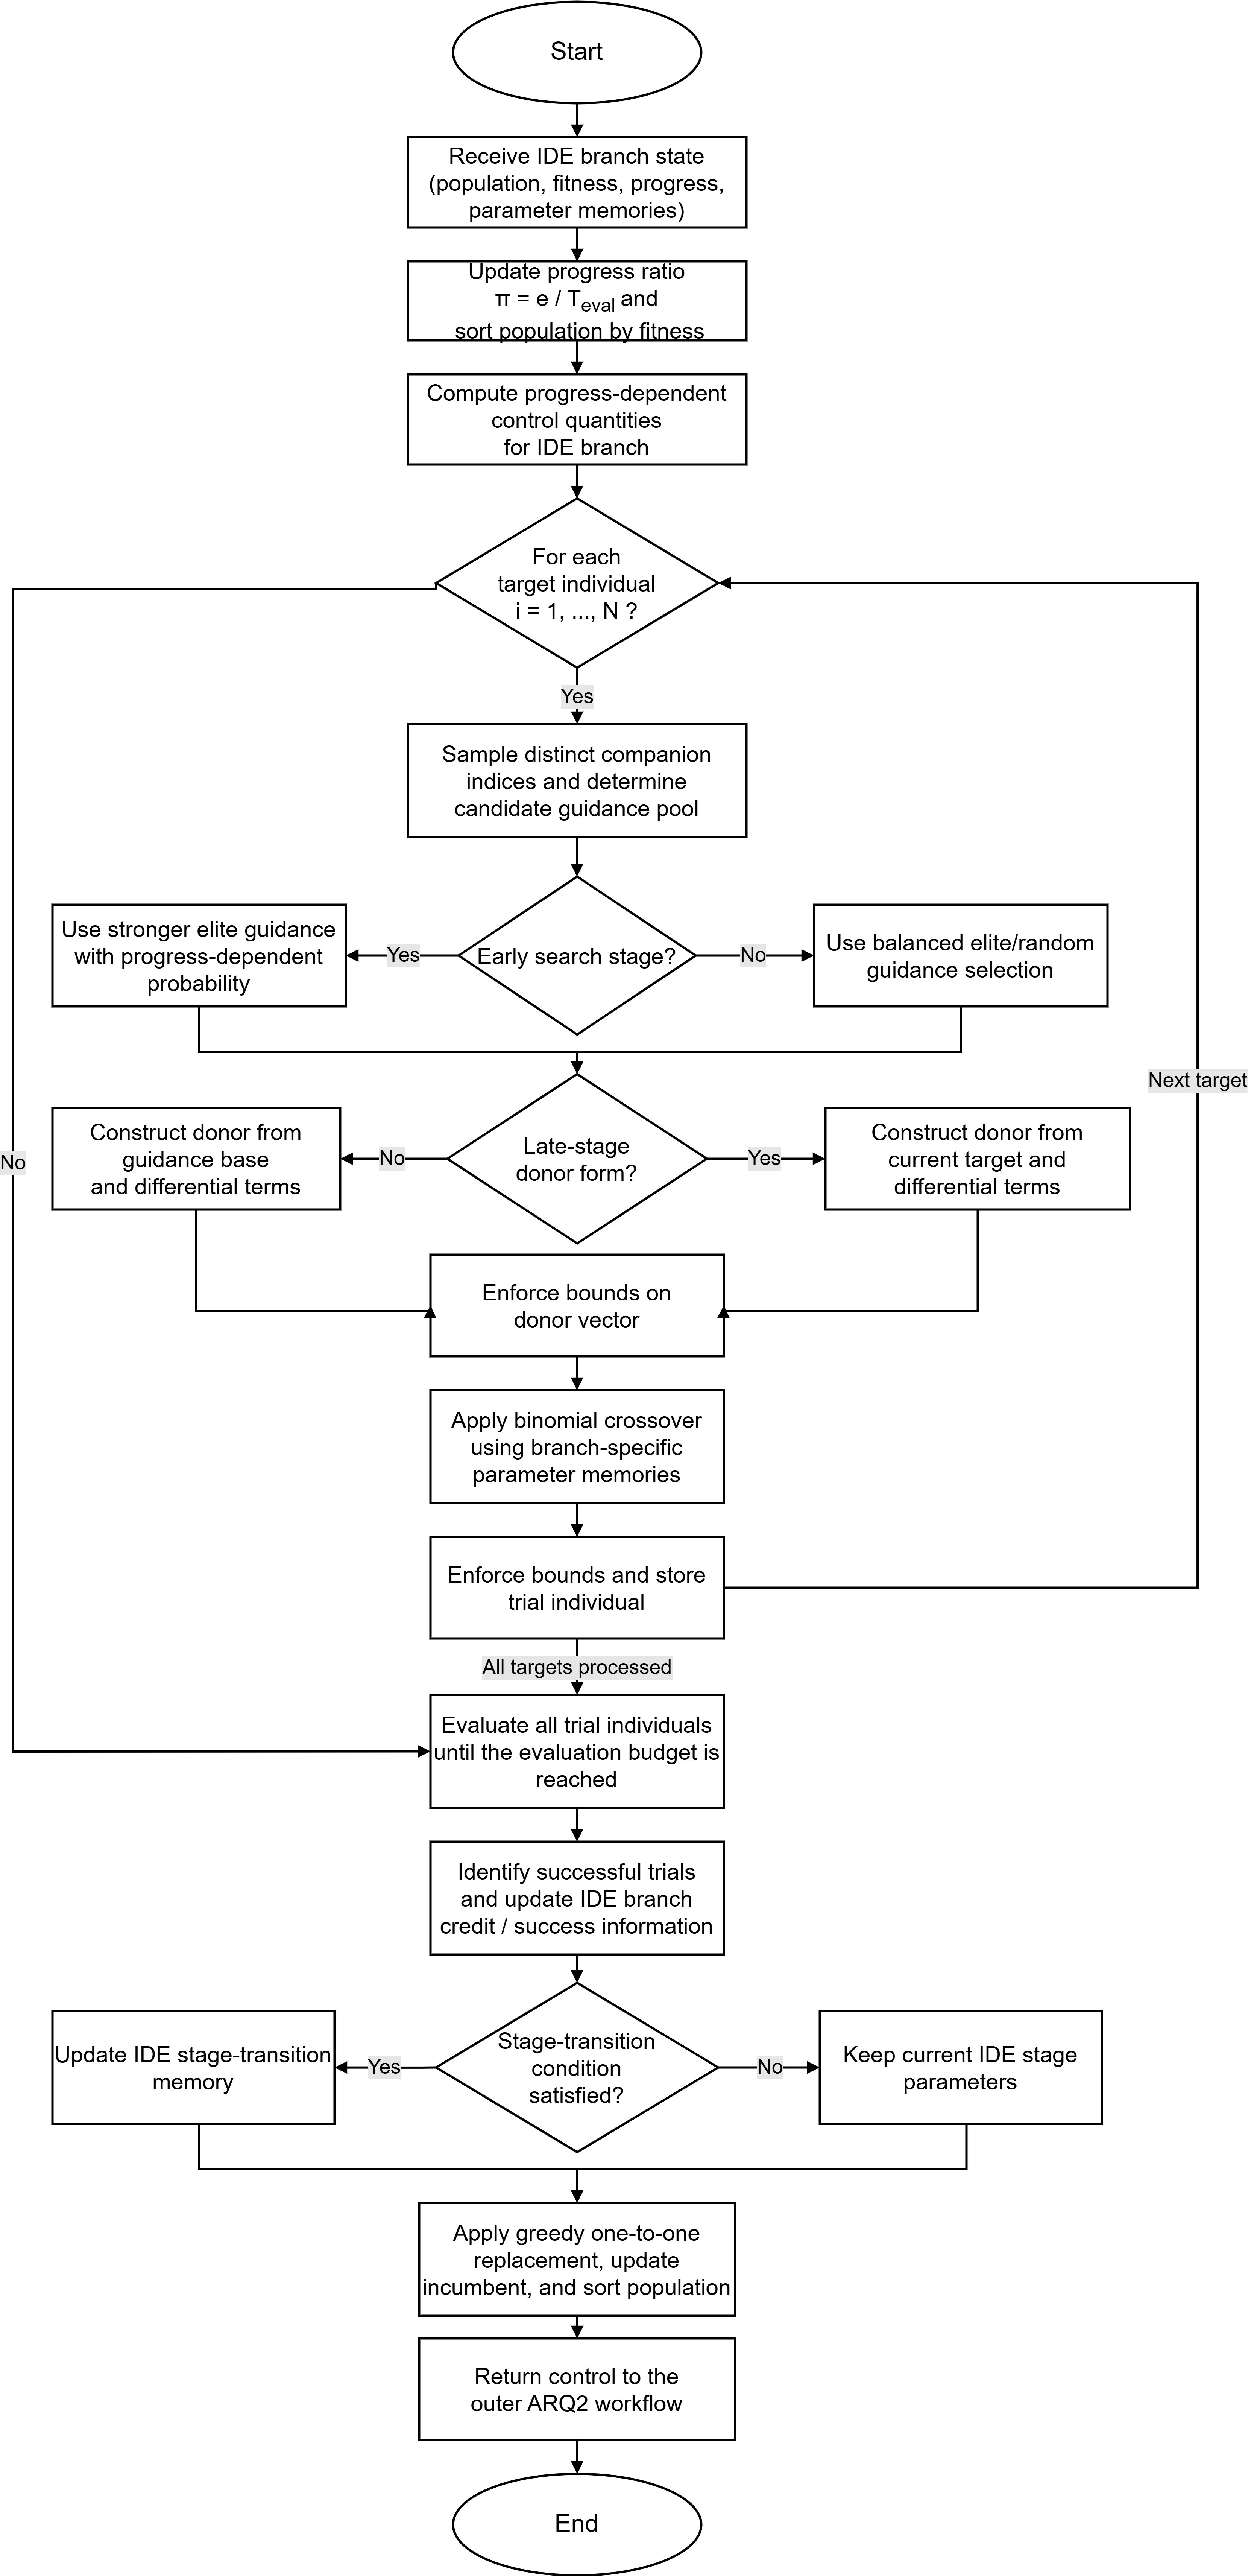
\includegraphics[scale=0.4]{arq2_ide_flow}
\par\end{centering}
\caption{IDE branch update in ARQ2\label{fig:ide}}
\end{figure}

\begin{algorithm}
INPUT

- $X=\{x_{i}\}_{i=1}^{N}$: current population

- $f$: objective function

- $\Omega$: feasible search domain

- $e,\ T_{\mathrm{eval}}$: current and maximum numbers of function
evaluations

- $\pi_{t}$: phase-switch progress threshold

- $\lambda,\ \lambda_{c}$: patience window and consecutive low-success
counter

- $\{F_{i}^{\mathrm{IDE}},CR_{i}^{\mathrm{IDE}}\}_{i=1}^{N}$: individual
IDE parameter memories

- $n_{\mathrm{IDE}}$: credit of the IDE branch

OUTPUT

- Updated population, incumbent pair, IDE state, and IDE branch credit

IDE branch update in ARQ2

01 Set $\pi\leftarrow e/T_{\mathrm{eval}}$

02 Sort $X$ in nondecreasing objective value

03 Set $\varepsilon(\pi)\leftarrow0.1+0.9\cdot10^{5(\pi-1)}$

04 If $\pi<\pi_{t}$ then set $S_{\mathrm{th}}\leftarrow0$; otherwise
set $S_{\mathrm{th}}\leftarrow0.1$

05 For each $i=1,\ldots,N$ do

06 {\scriptsize\hspace{0.5cm}}Sample distinct indices $o,r_{1},r_{2},r_{3}\neq i$

07 {\scriptsize\hspace{0.5cm}}Set $m(\pi)\leftarrow\max\{2,\mathrm{round}(\varepsilon(\pi)N)\}$

08 {\scriptsize\hspace{0.5cm}}If $\pi\leq\pi_{t}$ then

09 {\scriptsize\hspace{0.5cm}\hspace{0.5cm}}With probability $0.9\varepsilon(\pi)$,
choose $r_{1}^{\star}$ from the best $m(\pi)$ individuals; otherwise
set $r_{1}^{\star}\leftarrow r_{1}$

10 {\scriptsize\hspace{0.5cm}}Else

11 {\scriptsize\hspace{0.5cm}\hspace{0.5cm}}With probability $0.5$,
choose $r_{1}^{\star}$ from the best $m(\pi)$ individuals; otherwise
set $r_{1}^{\star}\leftarrow r_{1}$

12 {\scriptsize\hspace{0.5cm}}Endif

13 {\scriptsize\hspace{0.5cm}}If $\pi>\pi_{t}$ and a Bernoulli trial
with parameter $0.5$ succeeds then

14 {\scriptsize\hspace{0.5cm}\hspace{0.5cm}}Set $v_{i}\leftarrow x_{i}+F_{i}^{\mathrm{IDE}}(x_{r_{1}^{\star}}-x_{o})+F_{i}^{\mathrm{IDE}}(x_{r_{2}}-x_{r_{3}})$

15 {\scriptsize\hspace{0.5cm}}Else

16 {\scriptsize\hspace{0.5cm}\hspace{0.5cm}}Set $v_{i}\leftarrow x_{o}+F_{i}^{\mathrm{IDE}}(x_{r_{1}^{\star}}-x_{o})+F_{i}^{\mathrm{IDE}}(x_{r_{2}}-x_{r_{3}})$

17 {\scriptsize\hspace{0.5cm}}Endif

18 {\scriptsize\hspace{0.5cm}}Repair $v_{i}$ to $\Omega$

19 {\scriptsize\hspace{0.5cm}}Construct trial vector $y_{i}$ by
binomial crossover between $x_{i}$ and $v_{i}$ with rate $CR_{i}^{\mathrm{IDE}}$

20 {\scriptsize\hspace{0.5cm}}Repair $y_{i}$ to $\Omega$, evaluate
$f(y_{i})$, and update $e$

21 Endfor

22 Define the success set $I_{s}=\{i:\ f(y_{i})<f(x_{i})\}$

23 Set $SR\leftarrow|I_{s}|/N$

24 Increase $n_{\mathrm{IDE}}$ in proportion to the number of successful
replacements

25 If $\pi<\pi_{t}$ then

26 {\scriptsize\hspace{0.5cm}}If $SR\leq S_{\mathrm{th}}$ then set
$\lambda_{c}\leftarrow\lambda_{c}+1$; otherwise set $\lambda_{c}\leftarrow0$

27 {\scriptsize\hspace{0.5cm}}If $\lambda_{c}\geq\lambda$ then set
$\pi_{t}\leftarrow\pi$

28 Endif

29 For each $i\in I_{s}$ do

30 {\scriptsize\hspace{0.5cm}}Replace $x_{i}$ with $y_{i}$

31 {\scriptsize\hspace{0.5cm}}Update the incumbent pair $(x^{\ast},f^{\ast})$
if improved

32 Endfor

33 Return the updated IDE state and population

\caption{IDE branch update in ARQ2\label{alg:ide}}

\end{algorithm}

If the selected branch is IDE, the method applies a progress-dependent
differential update with branch-specific memories for mutation and
crossover control. To preserve notation consistency with the rest
of the manuscript, the IDE-side behavior is also expressed through
the same global progress ratio $\pi$. The branch first defines the
progress-sensitive elite-pressure term

\[
\varepsilon_{\mathrm{IDE}}(\pi)=0.1+0.9\cdot10^{5(\pi-1)}.
\]

This quantity determines the size of the elite-guided pool,

\[
H(\pi)=\max\{2,\mathrm{round}(\varepsilon_{\mathrm{IDE}}(\pi)N)\}.
\]

Accordingly, the donor construction follows a progress-dependent mixed
strategy. In its guidance-oriented regime, the branch uses

\[
v_{i}=x_{o}+F_{i}(x_{r_{1}}-x_{o})+F_{i}(x_{r_{2}}-x_{r_{3}}),
\]

where $x_{r_{1}}$ is selected either from the elite pool of size
$H(\pi)$ or from a standard random index. In the later current-based
regime, it may instead use

\[
v_{i}=x_{i}+F_{i}(x_{r_{1}}-x_{o})+F_{i}(x_{r_{2}}-x_{r_{3}}).
\]

The trial vector is then generated by the same binomial crossover
form as above, but with branch-specific crossover memory $CR_{i}$.
After evaluation, the IDE branch applies greedy one-to-one replacement.
Denoting the offspring by $u_{i}$, replacement occurs when

\[
f(u_{i})\leq f(x_{i}),
\]

or, in the strict variant, when $f(u_{i})<f(x_{i})$. The IDE-side
success rate is then

\[
SR=\frac{|S|}{N},
\]

where $S$ is the set of successful offspring. Therefore, within ARQ2,
IDE acts as a complete complementary search routine rather than as
a single isolated mutation formula.

After branch execution, additional stabilization is applied only when
the selected branch is ARQ. The first layer is quarantine-based correction.
Let $Q_{3}$ denote the third quartile of the fitness distribution
and let $IQR$ denote the interquartile range. Fitness outliers are
identified through

\[
\theta=Q_{3}+\alpha_{Q}\cdot IQR,
\]

where $\alpha_{Q}$ is the outlier-sensitivity coefficient. A fraction
$\rho_{Q}$ of the detected outliers is then relocated around the
center of the better half of the population using Gaussian perturbations
scaled by $\sigma_{Q}$. The second layer is an ARQ-only micro-restart
activated when

\[
s\geq\tau,
\]

where $\tau$ is the stagnation threshold. In that case, the method
perturbs the incumbent neighborhood and attempts to replace the worst
fraction $\omega$ of the population using Gaussian noise scaled by
$\sigma_{R}$.

Finally, the iteration ends with a second archive-trimming stage,
followed by the update of the stopping state and the reporting of
the current incumbent. Consequently, the execution order of ARQ2 is:
archive maintenance, bootstrap-or-roulette scheduling, optional controller
reset, execution of the selected branch, ARQ-only stabilization when
applicable, and final bookkeeping. This hierarchy also defines the
natural order in which the overall flowchart, the roulette-based flowchart,
the IDE flowchart, and the three corresponding pseudocodes should
appear in the manuscript.

\section{Empirical Evaluation Protocol and Benchmark Landscape\label{sec:experiments}}

\subsection{Experimental Configuration and Reproducibility Protocol\label{subsec:generalsettings}}

All algorithms, including the proposed method and the baseline competitors,
were implemented in efficient ANSI C++ and integrated into the open-source
OptimSolution framework, which was created by Vasileios Charilogis.
The source code is publicly available through the GitHub repository:
\url{https://github.com/charilog/optimsolution} (accessed: 16 March
2026). Compilation and execution were carried out under Debian 12.12
using GCC 13.4. The experimental platform was a high-performance system
equipped with an AMD Ryzen 9 9950X3D processor (16 cores, 32 threads)
and 64 GB of DDR4 memory, also running Debian Linux. To capture the
stochastic behavior of the methods, each benchmark function was executed
in 30 independent runs with different random seeds, while the same
fixed objective-function evaluation budget was enforced for all solvers.
The budget of 150,000 function evaluations follows the termination
criterion established by the CEC 2011 real-world numerical optimization
benchmark suite \citep{cec2011}, ensuring direct comparability with
related literature. For higher-dimensional problems such as test2n
(D=200), this budget is more restrictive but is retained deliberately
so that all methods operate under a uniform computational constraint.
The primary reported performance measures were the best and mean objective
values obtained at termination, computed over the 30 independent runs
for each test problem. In the comparative tables, first-ranked entries
are highlighted in green and second-ranked entries in blue, while
all parameter settings follow exactly the values reported in Tables
\ref{tab:parameter1} and \ref{tab:parametes2}. Although some competitors
such as JSO employ a variable initial population size determined by
a problem-dimension-dependent factor, fairness across all compared
methods is ensured at the level of the total function evaluation budget
rather than at the level of population size. Since all solvers are
subject to the same fixed limit of 150,000 function evaluations, differences
in population initialization strategy affect only the internal allocation
of that budget and do not grant any method an additional computational
advantage. To ensure a fair comparison on equal computational terms,
local search components embedded in certain competitors were disabled
in the present experimental setting. Specifically, the eigenvector-based
local refinement of EA4Eig was deactivated, as it introduces an additional
layer of exploitation that is absent from the remaining methods and
would otherwise render the comparison asymmetric with respect to the
per-evaluation computational effort.
\begin{center}
\begin{table}[H]
\centering
\caption{ARQ2 parameter settings used in the experiments\label{tab:parameter1}}

\begin{tabular}{lcl}
\hline 
Name & Value & Description\tabularnewline
\hline 
\hline 
$N$ & 100 & Population size\tabularnewline
\hline 
$T_{\mathrm{eval}}$ & 150,000 & Maximum number of function evaluations\tabularnewline
\hline 
$p$ & 0.12 & Top fraction for p-best selection in the ARQ branch\tabularnewline
\hline 
$\xi$ & 0.60 & Agent-update fraction in the ARQ branch\tabularnewline
\hline 
$\mu_{F}$ & 0.60 & Initial mean of the scaling factor in the ARQ branch\tabularnewline
\hline 
$\mu_{CR}$ & 0.85 & Initial mean of the crossover rate in the ARQ branch\tabularnewline
\hline 
$F_{lo}$ & 0.05 & Lower bound imposed on the ARQ scaling factor\tabularnewline
\hline 
$F_{hi}$ & 1.40 & Upper bound imposed on the ARQ scaling factor\tabularnewline
\hline 
$\alpha_{Q}$ & 1.0 & Outlier-sensitivity coefficient in the quarantine stage\tabularnewline
\hline 
$\rho_{Q}$ & 0.08 & Fraction of detected outliers repaired by quarantine\tabularnewline
\hline 
$\sigma_{Q}$ & 0.10 & Gaussian perturbation scale used in quarantine\tabularnewline
\hline 
$\omega$ & 0.08 & Worst-population fraction used in the ARQ micro-restart\tabularnewline
\hline 
$\sigma_{R}$ & 0.18 & Gaussian perturbation scale used in the ARQ micro-restart\tabularnewline
\hline 
$\tau$ & 24 & Stagnation threshold for triggering the ARQ micro-restart\tabularnewline
\hline 
$\eta_{SH}$ & 0.10 & Success-history smoothing coefficient in the ARQ branch\tabularnewline
\hline 
$\alpha_{A}$ & 1.5 & Archive-size coefficient\tabularnewline
\hline 
$r_{RTR}$ & 14 & Candidate-pool size used by restricted tournament replacement\tabularnewline
\hline 
$h$ & 2 & Number of internal branches in the roulette controller\tabularnewline
\hline 
$n_{0}$ & 2 & Baseline credit assigned to each branch\tabularnewline
\hline 
$\delta$ & 0.10 & Controller reset threshold\tabularnewline
\hline 
$b$ & 2 & Bootstrap length during which the ARQ branch is enforced\tabularnewline
\hline 
$\pi_{t}^{(0)}$ & 0.5 & Initial phase-switch threshold in the IDE branch\tabularnewline
\hline 
$\lambda$ & 150 & Patience window in the IDE branch\tabularnewline
\hline 
\end{tabular}
\end{table}
\begin{table}[H]
\centering
\caption{Parameters of other methods\label{tab:parametes2}}

\centering{}%
\begin{tabular}{lcV{\linewidth}}
\hline 
Name & Value & Description\tabularnewline
\hline 
\hline 
$N$ & 100 & Population size for all methods\tabularnewline
\hline 
\multicolumn{3}{c}{JSO}\tabularnewline
\hline 
$NP_{factor}$ & 18 & Initial population size $NP_{0}=NP_{factor}\times Dim$\tabularnewline
\hline 
$H$ & 20 & Memory size for success-history means $MF$/$MCR$\tabularnewline
\hline 
$pbest$ & 0.11 & Fraction for p-best selection (top-p set).\tabularnewline
\hline 
$archive_{rate}$ & 1 & Archive size as multiple of NP0

(i.e., archiveMax = archive\_rate \texttimes{} NP0).\tabularnewline
\hline 
\multicolumn{3}{c}{CLPSO}\tabularnewline
\hline 
$cl_{p}$ & 0.3 & Comprehensive learning probability\tabularnewline
\hline 
$cognitive_{weight}$ & 1.49445 & Cognitive weight\tabularnewline
\hline 
$inertia_{weight}$ & 0.729 & Inertia weight\tabularnewline
\hline 
$mutation_{rate}$ & 0.01 & Mutation rate\tabularnewline
\hline 
$social_{weight}$ & 1.49445 & Social weight\tabularnewline
\hline 
\multicolumn{3}{c}{EA4Eig}\tabularnewline
\hline 
$archive_{size}$ & 100 & Archive size for JADE-style mutation\tabularnewline
\hline 
$eig_{interval}$ & 5 & Recompute eigenbasis every k iterations\tabularnewline
\hline 
$CR_{max}$ & 1 & Upper bound for $CR$\tabularnewline
\hline 
$F_{max}$ & 1 & Upper bound for $F$\tabularnewline
\hline 
$CR_{min}$ & 0 & Lower bound for $CR$\tabularnewline
\hline 
$F_{min}$ & 0.1 & Lower bound for $F$\tabularnewline
\hline 
$p_{best}$ & 0.2 & pbest fraction (current-to-pbest/1/bin)\tabularnewline
\hline 
$CR_{tau}$ & 0.1 & Self-adaptation prob. for $CR$\tabularnewline
\hline 
$F_{tau}$ & 0.1 & Self-adaptation prob. for $F$\tabularnewline
\hline 
\multicolumn{3}{c}{mLSHADE\_RL}\tabularnewline
\hline 
$archive_{size}$ & 500 & Archive size\tabularnewline
\hline 
$Memory_{size}$ & 10 & Success-history memory size\tabularnewline
\hline 
$Population_{min}$ & 4 & Minimum population size\tabularnewline
\hline 
$p_{best_{max}}$ & 0.2 & Maximum pbest fraction\tabularnewline
\hline 
$p_{best_{min}}$ & 0.05 & Minimum pbest fraction\tabularnewline
\hline 
\multicolumn{3}{l}{SaDE}\tabularnewline
\hline 
$CR_{sigma}$ & 0.1 & Std for $CR$ sampling\tabularnewline
\hline 
$F_{gamma}$ & 0.1 & Scale for Cauchy $F$ sampling\tabularnewline
\hline 
$CR_{init}$ & 0.5 & Initial $CR$ mean\tabularnewline
\hline 
$F_{init}$ & 0.7 & Initial $F$ mean\tabularnewline
\hline 
$learning_{period}$ & 25 & Iterations per adaptation window\tabularnewline
\hline 
\multicolumn{3}{c}{UDE3}\tabularnewline
\hline 
$Population_{min}$ & 4 & Minimum population size.\tabularnewline
\hline 
$Memory_{size}$ & 10 & Success-history memory size\tabularnewline
\hline 
$archive_{size}$ & 100 & Archive size\tabularnewline
\hline 
$p_{best_{min}}$ & 0.05 & Minimum pbest fraction\tabularnewline
\hline 
$p_{best_{max}}$ & 0.2 & Maximum pbest fraction.\tabularnewline
\hline 
\multicolumn{3}{c}{TRIDENT-DE: See Table 1 here \citep{Charilogis2}}\tabularnewline
\hline 
\end{tabular}
\end{table}
\par\end{center}

\subsection{Real-World and Classic Optimization Testbed \label{subsec:problems}}

Section \ref{subsec:problems} is structured around two complementary
benchmark groups \ref{realworldfunctions} and \ref{nonrealworldfunctions}.
The first group consists of real-world optimization problems and is
included to evaluate the practical utility of ARQ2 under constrained,
black-box, simulator-driven, and application-oriented conditions.
The second group consists of classical hard benchmark functions and
is used to examine core search behavior under controlled settings,
including multimodality, ruggedness, ill-conditioning, separability
or non-separability, and sensitivity to increasing dimensionality.
The joint use of these two benchmark categories reduces the risk of
drawing conclusions from a single problem family and supports a more
balanced assessment of ARQ2, both in terms of practical applicability
and in terms of fundamental robustness across heterogeneous optimization
landscapes..

\medskip{}


\subsubsection{\textbf{\uline{Real world benchmark functions:\label{realworldfunctions}}}}
\begin{itemize}
\item \textbf{Uniform Linear Antenna Array Design (half-wavelength spacing,
amplitude taper) {[}antennaarray{]} \citep{antennaarrayantennaula}}

Objective:

$AF(\theta)=\sum_{n=0}^{N-1}w_{n}e^{j\pi n\cos(\theta)},\quad\widehat{AF}(\theta)=\frac{|AF(\theta)|}{\sum_{n=0}^{N-1}w_{n}}.$

$f(w)=5\left(1-\widehat{AF}(0)\right)^{2}+\frac{1}{|\Theta_{\mathrm{sll}}|}\sum_{\theta\in\Theta_{\mathrm{sll}}}|\widehat{AF}(\theta)|^{4}+0.01\sum_{n=0}^{N-2}(w_{n+1}-w_{n})^{2}.$

Dimension: 6

Bounds: $x_{i}\in[-6.4,6.35]$
\item \textbf{Uniform Linear Array (half-wavelength spacing, amplitude taper)
{[}antennaula{]} \citep{antennaarrayantennaula}}

Objective:

$f(w)=5\left(1-AF_{\mathrm{norm}}(0)\right)^{2}+\frac{1}{|\Theta_{\mathrm{sll}}|}\sum_{\theta\in\Theta_{\mathrm{sll}}}|AF_{\mathrm{norm}}(\theta)|^{4}+0.01\sum_{n=0}^{N-2}(w_{n+1}-w_{n})^{2}$

Dimension: 10

Bounds: $w_{n}\in[0,1],\quad n=0,1,\dots,N-1$
\item \textbf{Bifunctional Catalyst Blend Optimal Control (1D control) {[}bifunctionalcatalyst{]}
\citep{bifunctionalcatalyst1,bifunctionalcatalyst2,bifunctionalcatalyst3}}

\textbf{Vars:} catalyst blend $u(t)$ along the reactor

\textbf{Bounds:} $0.6\le u(t)\le0.9$.\\
\textbf{States:} $x_{1},\ldots,x_{7}$ (mole fractions) governed b

$\dot{x}_{1}=-k_{1}x_{1},\quad\dot{x}_{2}=k_{1}x_{1}-(k_{2}{+}k_{3})x_{2}+k_{4}x_{5},\quad\dot{x}_{3}=k_{2}x_{2},\quad\dot{x}_{4}=-k_{6}x_{4}+k_{5}x_{5},$

$\dot{x}_{5}=-k_{3}x_{2}+k_{6}x_{4}-(k_{4}{+}k_{5}{+}k_{6})x_{5}+k_{7}x_{6}+k_{10}x_{7},\quad\dot{x}_{6}=k_{8}x_{5}-k_{9}x_{6},\quad\dot{x}_{7}=k_{9}x_{5}-k_{10}x_{7},$

with $k_{i}=c_{i1}+c_{i2}u+c_{i3}u^{2}+c_{i4}u^{3}$ (coefficients
$c_{ij}$ given) and $x(0)=[1,0,0,0,0,0,0]^{\top}$.\\
 \textbf{Objective:} maximize benzene at outlet $J=10^{3}x_{7}(t_{f})$,
we minimize $-J$.

Dimension: 1

Bounds: $u\in[0.6,0.9]$
\item \textbf{Dynamic Economic Dispatch 1 {[}ded1{]} \citep{cec2011}}

Objective:

$\min_{\mathbf{P}}\quad f(\mathbf{P})=\sum_{t=1}^{24}\sum_{i=1}^{5}\left(a_{i}P_{i,t}^{2}+b_{i}P_{i,t}+c_{i}\right)$

$P_{i}^{\min}\leq P_{i,t}\leq P_{i}^{\max},\quad\forall i=1,\ldots,5,\;t=1,\ldots,24$

$\sum_{i=1}^{5}P_{i,t}=D_{t},\quad\forall t=1,\ldots,24$

$P_{\min}=[10,20,30,40,50]$

$P_{\max}=[75,125,175,250,300]$

Dimension: 10

Bounds: $P_{i}^{\min}\leq P_{i,t}\leq P_{i}^{\max}$
\item \textbf{Dynamic Economic Dispatch 2 {[}ded2{]} \citep{cec2011}}

Objective:

$\min_{\mathbf{P}}\quad f(\mathbf{P})=\sum_{t=1}^{24}\sum_{i=1}^{9}\left(a_{i}P_{i,t}^{2}+b_{i}P_{i,t}+c_{i}\right)$

$P_{i}^{\min}\leq P_{i,t}\leq P_{i}^{\max},\quad\forall i=1,\ldots,5,\;t=1,\ldots,24$

$\sum_{i=1}^{5}P_{i,t}=D_{t},\quad\forall t=1,\ldots,24$

$P_{\min}=[150,135,73,60,73,57,20,47,20]$

$P_{\max}=[470,460,340,300,243,160,130,120,80]$

Dimension: 10

Bounds: $P_{i}^{\min}\leq P_{i,t}\leq P_{i}^{\max}$
\item \textbf{Static Economic Load Dispatch 1, 2, 3, 4 and 5 {[}eld{]} \citep{cec2011}}

Objective:

$\min_{P_{1},\ldots,P_{N_{G}}}F=\sum_{i=1}^{N_{G}}f_{i}(P_{i})$

$f_{i}(P_{i})=a_{i}P_{i}^{2}+b_{i}P_{i}+c_{i},\quad i=1,2,\ldots,N_{G}$

$f_{i}(P_{i})=a_{i}P_{i}^{2}+b_{i}P_{i}+c_{i}+|e_{i}\sin(f_{i}(P_{i}^{\min}-P_{i}))|$

$P_{i}^{\min}\leq P_{i}\leq P_{i}^{\max},\quad i=1,2,\ldots,N_{G}$

$\sum_{i=1}^{N_{G}}P_{i}=P_{D}+P_{L}$

$P_{L}=\sum_{i=1}^{N_{G}}\sum_{j=1}^{N_{G}}P_{i}B_{ij}P_{j}+\sum_{i=1}^{N_{G}}B_{0i}P_{i}+B_{00}$

$P_{i}-P_{i}^{0}\leq UR_{i}\quad P_{i}^{0}-P_{i}\leq DR_{i}$

Dimension: 6, 13, 15, 40, 140

Bounds: See Technical Report of CEC2011
\item \textbf{Idealized gas cycle efficiency (Brayton-type) {[}gascycle{]}
\citep{cec2011}}

Objective:

Let $\gamma=1.4$ and pressure ratio$r=P_{3}/P_{1}$.The cycle efficiency
is

$\eta=1-\frac{1}{r^{(\gamma-1)/\gamma}}\frac{T_{1}}{T_{3}}.$

Since the framework performs minimization, the optimized objective
is $f(x)=-\eta.$

Dimension: Intrinsic dimension: $D=4$

Decision variables:
\begin{itemize}
\item $x_{1}=T_{1}$ : inlet temperature.
\item $x_{2}=T_{3}$ : turbine inlet temperature.
\item $x_{3}=P_{1}$ : low pressure.
\item $x_{4}=P_{3}$ : high pressure
\end{itemize}
Bounds: $300\leq T_{1}\leq1500,$$1200\leq T_{3}\leq2000,$$1\leq P_{1}\leq20,\qquad1\leq P_{3}\leq20.$
\item \textbf{Hydrothermal scheduling (smooth penalty model) {[}hydrothermal{]}
\citep{cec2011}}

Objective:

Reservoir dynamics:

$V_{j,t+1}=V_{j,t}+I_{j,t}-Q_{j,t}.$

Mid-step storage and hydro power:

$\bar{V}_{j,t}=\frac{V_{j,t}+V_{j,t+1}}{2},\qquad H_{j,t}=\kappa_{j}\left(h_{0,j}+\beta_{j}\bar{V}_{j,t}\right)Q_{j,t}.$

Objective:

$f(x)=\sum_{t=1}^{24}\sum_{i=1}^{3}\left(a_{i}P_{i,t}^{2}+b_{i}P_{i,t}+c_{i}\right)+w_{bal}\sum_{t=1}^{24}\left(\sum_{i=1}^{3}P_{i,t}+\sum_{j=1}^{2}H_{j,t}-D_{t}\right)^{2}+$

$w_{V}\,\Phi_{V}+w_{QP}\,\Phi_{QP}+w_{final}\sum_{j=1}^{2}\left(V_{j,24}-V_{j}^{final}\right)^{2}$

Penalty weights:$w_{bal}=0.1$,$w_{V}=5.0$,$w_{QP}=1.0$,$w_{final}=10.0$.

Dimension: $D=NG\cdot T+NH\cdot T=3\cdot24+2\cdot24=120$

Bounds: 
\begin{itemize}
\item $P_{1,t}\in[50,200],\quad P_{2,t}\in[60,250],\quad P_{3,t}\in[100,300].$
\item $Q_{1,t}\in[20,100],\quad Q_{2,t}\in[25,120].$
\item $V_{j,t}\in[100,500],\quad V^{init}=[200,250],\quad V^{final}=[200,250].$
\end{itemize}
\item \textbf{ik6dof (PUMA 560 real-world IK) {[}ik6dof{]} \citep{ik6dof}}

Objective:

$\min_{q\in\Omega}f(q)=\|p(q)-p^{*}\|_{2}^{2}+\lambda\|\phi(q)-\phi^{*}\|_{2}^{2}$

Dimnsion: 6.

Bounds: 
\begin{itemize}
\item $\Omega=[-2.7925,2.7925]\times[-1.9199,1.9199]\times[-2.3562,2.3562]\times[-4.6426,4.6426]\times[-1.7453,1.7453]\times[-4.6426,4.6426]$
\item In degrees: $[-160,160],\ [-110,110],\ [-135,135],\ [-266,266],$
$\ [-100,100],\ [-266,266]$
\end{itemize}
\item \textbf{Minimum-Delta-V Interplanetary Trajectory Optimization for
the Messenger Spacecraft {[}messenger{]} \citep{messengertandem}}

Objective:

$\min f(x)=dV_{total}.$

$dV_{total}=dV_{launch}+dV_{legs}+dV_{DSM\_cost}+dV_{Mercury}-dV_{DSM\_help}-dV_{Venus\_gain}+P.$

$dV_{launch}=\max\left(6.5,\;10.0-2.5\log\left(1+\frac{T_{1}}{180}\right)\right).$

$dV_{legs}=\sum_{i=1}^{5}16\,\frac{1}{1+2r_{i}},\qquad r_{i}=\mathrm{clamp}\left(\frac{T_{i}}{220},0.25,4\right).$

$dV_{Mercury}=6\,\frac{1}{\sqrt{\mathrm{clamp}(T_{5}/300,0.2,4)}}(1-0.3r_{p})(1-0.2(k_{1}+k_{2})).$

Soft penalty:$P=0.008\,(T_{1}+T_{2}+T_{3}+T_{4}+T_{5}-1400)$ for
total time above$1400$ days, plus hard bound penalties.

Dimension: 14

Decision vector: $x=(t_{0},T_{1},T_{2},T_{3},T_{4},T_{5},s_{1},s_{2},s_{3},s_{4},s_{5},r_{p},k_{1},k_{2}).$

Bounds: $t_{0}\in[7000,10000],\quad T_{1}\in[30,400],\quad T_{2}\in[30,400],$$T_{3}\in[30,600],\quad T_{4}\in[30,600],\quad T_{5}\in[30,700],$$s_{1},\ldots,s_{5},r_{p},k_{1},k_{2}\in[0,1].$
\item \textbf{OFDM Power Allocation {[}ofdmpower{]} \citep{cec2011}}

Objective:

$f(p)=-\sum_{i=0}^{N-1}\log_{2}\left(1+\frac{h_{i}p_{i}}{N_{0}}\right)+w_{sum}\max\left(0,\sum_{i=0}^{N-1}p_{i}-P_{tot}\right)^{2}.$

Dimension: $D=N,\qquad N\geq2.$

Decision vector: $p=(p_{0},p_{1},\dots,p_{N-1}).$

Bounds: $0\leq p_{i}\leq P_{max}=1,\qquad i=0,1,\dots,N-1.$

Channel profile: $h_{i}=\frac{1}{1+\alpha i},\qquad\alpha=0.15.$
For $N\geq3$, the code applies small deterministic corrections to
$h_{\lfloor N/3\rfloor}$ and $h_{\lfloor2N/3\rfloor}$.
\item \textbf{Spread Spectrum Radar Polyphase Code Design {[}polyphase{]}
\citep{polyphase}}

Objective:

$\min_{x\in X}\;f(x)=\max\left\{ |\varphi_{1}(x)|,|\varphi_{2}(x)|,\ldots,|\varphi_{m}(x)|\right\} $

$X=\{x\in\mathbb{R}^{n}\mid0\leq x_{j}\leq2\pi,\;j=1,\ldots,n\}m=2n-1$

$\varphi_{j}(x)=\begin{cases}
{\displaystyle \sum_{k=1}^{n-j}\cos(x_{k}-x_{k+j})} & \text{for }j=1,\ldots,n-1\\
{\displaystyle n} & \text{for }j=n\\
{\displaystyle \varphi_{2n-j}(x)} & \text{for }j=n+1,\ldots,2n-1
\end{cases}$

$\varphi_{j}(x)=\sum_{k=1}^{n-j}\cos(x_{k}-x_{k+j}),\quad j=1,\ldots,n-1$

$\varphi_{n}(x)=n$, $\varphi_{n+\ell}(x)=\varphi_{n-\ell}(x),\quad\ell=1,\ldots,n-1$

Dimension: 20

Bounds: $x_{j}\in[0,2\pi]$
\item \textbf{Lennard-Jones Potential {[}potential{]} \citep{potential}}

Oblective:

$\min_{x\in\mathbb{R}^{3N-6}}\;f(x)=4\sum_{i=1}^{N-1}\sum_{j=i+1}^{N}\left[\left(\frac{1}{r_{ij}}\right)^{12}-\left(\frac{1}{r_{ij}}\right)^{6}\right]$

Dimension: 38

Bounds: 
\begin{itemize}
\item $x_{0}\in(0,0,0)$
\item $x_{1},x_{2}\in[0,4]$
\item $x_{3}\in[0,\pi]$
\item $x_{3k-3}$
\item $x_{3k-2}$
\item $x_{i}\in[-b_{k},+b_{k}]$
\end{itemize}
\item \textbf{Markowitz Mean-Variance Portfolio (long-only, soft sum-to-one)
{[}portfoliomv{]} \citep{portfoliomv}}

Objective: 

$f(w)=w_{\mathrm{risk}}\left(w^{T}\Sigma w\right)-w_{\mathrm{ret}}\left(\mu^{T}w\right)+w_{\mathrm{sum}}\left(\sum_{i=0}^{N-1}w_{i}-1\right)^{2}.$

$w_{\mathrm{risk}}=1,\qquad w_{\mathrm{ret}}=0.5,\qquad w_{\mathrm{sum}}=50.$

Dimension: $D=N,\qquad N\geq2.$

Decision vector: $w=\left[w_{0},w_{1},\dots,w_{N-1}\right]^{T}.$

Bounds: $0\leq w_{i}\leq1,\qquad i=0,1,\dots,N-1.$

Expected-return profile: $\mu_{i}=0.02+0.06\frac{i}{N-1},\qquad i=0,1,\dots,N-1.$

Covariance model: $\sigma_{i}=0.20\left(1+0.2\frac{i}{N-1}\right),$$\Sigma_{ij}=\sigma_{i}\sigma_{j}\rho^{\left|i-j\right|}+10^{-6}\delta_{ij},\qquad\rho=0.3.$
\item \textbf{Space Trajectory: TANDEM (MGA-1DSM Surrogate) {[}tandem{]}
\citep{messengertandem}}
\begin{lyxlist}{}
\item [{Objective:}]~
\item [{$\min_{\mathbf{x}}\ \Delta V_{\text{tot}}=\Delta V_{\text{launch}}(T_{1})+\sum_{i=1}^{4}\Delta V_{\text{leg}}(T_{i})+\Delta V_{\text{branch}}(T_{5A},s_{5A},k_{A1},k_{A2})+$}]~
\item [{$\Delta V_{\text{branch}}(T_{5B},s_{5B},k_{B1},k_{B2})\quad+\sum_{i=1}^{4}\Delta V_{\text{DSM}}(s_{i})-$}]~
\item [{$G_{\text{GA}}(T_{1},T_{2},T_{3})-G_{\text{J}}(T_{4})+\Pi_{\text{ToF}}+\Pi_{\text{bounds}}.$}]~
\item [{\textit{Compact}}] \begin{flushleft}
\textit{component forms (surrogate):} $\Delta V_{\text{leg}}(T)=\ell_{s}/(1+2\,\mathrm{clip}(T/t_{r},0.2,4))$,
\par\end{flushleft}
\item [{$\Delta V_{\text{DSM}}(s)=c_{\text{DSM}}(0.25+0.75s)$,}] $\Delta V_{\text{branch}}(\cdot)$ 
\item [{adds}] DSM shaping terms with $r_{p},k_{\cdot}$, $G_{\text{GA}},G_{\text{J}}$are
decreasing functions of leg times, $\Pi_{\text{ToF}}=\beta\,[(T_{1}{+}T_{2}{+}T_{3}{+}T_{4}{+}\tfrac{1}{2}(T_{5A}{+}T_{5B}))-T_{\text{soft}}]_{+}$.
\item [{Dimension:}] 18, $\mathbf{x}=[t_{0},T_{1},T_{2},T_{3},T_{4},T_{5A},T_{5B},s_{1},s_{2},s_{3},s_{4},s_{5A},s_{5B},r_{p},k_{A1},k_{A2},k_{B1},k_{B2}]^{\top}$
\item [{Bounds:}] \begin{flushleft}
$t_{0}\in[7000,10000]$ (MJD2000 d), $T_{1}\in[30,500]$,
$T_{2}\in[30,600]$, $T_{3}\in[30,1200]$, $T_{4}\in[30,1600]$, $T_{5A},T_{5B}\in[30,2000]$
d, $s_{\bullet},r_{p},k_{\bullet}\in[0,1]$.
\par\end{flushleft}
\end{lyxlist}
\item \textbf{Tersoff Potential for model Si (B) {[}tersoffb{]} \citep{tersoffb}}

Objective:

$\min_{\mathbf{x}\in\Omega}f(\mathbf{x})=\sum_{i=1}^{N}E(\mathbf{x}_{i})$

$E(\mathbf{x}_{i})=\frac{1}{2}\sum_{j\neq i}f_{c}(r_{ij})\left[V_{R}(r_{ij})-B_{ij}V_{A}(r_{ij})\right]$

where $r_{ij}=\|\mathbf{x}_{i}-\mathbf{x}_{j}\|$, $V_{R}(r)=A\exp(-\lambda_{1}r)$

$V_{A}(r)=B\exp(-\lambda_{2}r)$

$f_{c}(r)$: cutoff function with $f_{c}(r)$: angle parameter

Dimension: 30

Bounds: $x_{1}\in[0,4]$$x_{2}\in[0,4]$ $x_{3}\in[0,\pi]$ $x_{i}\in\left[\frac{4(i-3)}{4},\ 4\right]$
\item \textbf{Tersoff Potential for model Si (C) {[}tersoffc{]} \citep{tersoffc}}

Objective:

$\min_{\mathbf{x}}\;V(\mathbf{x})=\sum_{i=1}^{N}\sum_{j>i}^{N}f_{C}(r_{ij})\left[a_{ij}f_{R}(r_{ij})+b_{ij}f_{A}(r_{ij})\right]$

$f_{C}(r)=\begin{cases}
1, & r<R-D\\
\frac{1}{2}+\frac{1}{2}\cos\left(\frac{\pi(r-R+D)}{2D}\right), & |r-R|\leq D\\
0, & r>R+D
\end{cases}$

$f_{R}(r)=A\exp(-\lambda_{1}r)$

$f_{A}(r)=-B\exp(-\lambda_{2}r)$

$b_{ij}=\left[1+(\beta^{n})\zeta_{ij}^{n}\right]^{-1/(2n)}$

$\sum_{k\neq i,j}f_{C}(r_{ik})g(\theta_{ijk})\exp\left[\lambda_{3}^{3}(r_{ij}-r_{ik})^{3}\right]$

Dimension: 30

Bounds: $x_{1}\in[0,4]$ $x_{2}\in[0,4]$ $x_{3}\in[0,\pi]$$x_{i}\in\left[\frac{4(i-3)}{4},\ 4\right]$
\item \textbf{Electricity Transmission Pricing {[}transmissionpricing{]}
\citep{transmissionpricing1,transmissionpricing2}}

Objective:

$\min_{x}\;\;f(x)=\sum_{i=1}^{N_{g}}\left(\frac{C_{i}^{gen}}{P_{i}^{gen}}-R_{i}^{gen}\right)^{2}+\sum_{j=1}^{N_{d}}\left(\frac{C_{j}^{load}}{P_{j}^{load}}-R_{j}^{load}\right)^{2}$

$\sum_{j}GD_{i,j}+\sum_{j}BT_{i,j}=P_{i}^{gen},\quad\forall i$

$\sum_{i}GD_{i,j}+\sum_{i}BT_{i,j}=P_{j}^{load},\quad\forall j$

$GD_{i,j}^{max}=\min(P_{i}^{gen}-BT_{i,j},\;P_{j}^{load}-BT_{i,j})$

Dimension: 126

Bounds: $GD_{i,j}\in[0,GD_{i,j}^{max}]$
\item \textbf{Base-excited SDOF isolation platform design {[}vibratingplatform{]}
\citep{cec2011}}

Objective:

$f(x)=\mathrm{avg}_{f\in[5,200]}|H(f)|^{2}+P_{\delta}+P_{disp}+P_{\zeta}+P_{f_{n}}.$

$\delta=\frac{mg}{k}\le\delta_{max},\qquad\delta_{max}=0.005\ \mathrm{m}.$

Work-frequency displacement constraint at $f_{work}=30$ Hz:

$X_{work}=|H(f_{work})|Y_{0}\le x_{max},\qquad Y_{0}=5\cdot10^{-4}\ \mathrm{m},\qquad x_{max}=2\delta_{max}.$

Decision variables:$x_{1}=k$: spring stiffness $[\mathrm{N/m}]$,
$x_{2}=c$: viscous damping $[\mathrm{N\,s/m}]$.

Dimension: 2 

Bounds: $k\in[10^{3},2\cdot10^{5}],\qquad c\in[50,5\cdot10^{3}].$

Additional soft bounds:$\zeta\in[0.02,0.30]$ and $f_{n}\in[2,20]$
Hz.

Penalty weights:$w_{\delta}=100$,$w_{disp}=100$,$w_{\zeta}=25$,$w_{f_{n}}=25$.

Derived quantities: $\omega_{n}=\sqrt{\frac{k}{m}},\qquad f_{n}=\frac{\omega_{n}}{2\pi},\qquad\zeta=\frac{c}{2\sqrt{km}}.$
with $m=50$ kg.
\item \textbf{Wireless Coverage Antenna Placement {[}wirelesscoverage{]}
\citep{wirelesscoverage}}

Objective:

$x_{i},\ y_{i}\in\mathbb{R}\quad(\text{position}),P_{i}\in\mathbb{R}_{\ge0}\quad(\text{transmission power}).$

$S_{iu}(x_{i},y_{i},P_{i})\;=\;\frac{G\,P_{i}}{\bigl(\,(x_{i}-x_{u})^{2}+(y_{i}-y_{u})^{2}\,\bigr)^{\alpha/2}+\varepsilon},$

$\min_{x,y,P}\;\underbrace{\sum_{u\in\mathcal{U}}\bigl[\tau-S_{u}(x,P)\bigr]_{+}}_{\text{coverage deficiency}}\;+\;\lambda_{P}\sum_{i=1}^{N}P_{i}\;+,$

$\;\lambda_{O}\sum_{u\in\mathcal{U}}\sum_{i<j}\bigl[\min\{S_{iu},S_{ju}\}-\kappa\bigr]_{+}$

$S_{u}(x,P)\;=\;\max_{i=1,\dots,N}\,S_{iu}(x_{i},y_{i},P_{i}).$

Dimension: 6

Bounds: $0\le x_{i}\le W,$ $0\le y_{i}\le H,$ $0\le P_{i}\le P_{\max}$

\medskip{}

\end{itemize}
%

\subsubsection{\textbf{\uline{Non Real world benchmark functions:\label{nonrealworldfunctions}}}}
\begin{itemize}
\item \textbf{Buche-Rastrigin function (BBOB-style variant) {[}bucherastrigin{]}
\citep{Varelas}}

Objective:

$f(x)=10D+\sum_{i=1}^{D}\left(z_{i}^{2}-10\cos\left(2\pi z_{i}\right)\right)$

$z_{i}=s_{i}x_{i},\qquad s_{i}=10^{\frac{1}{2}\frac{i-1}{D-1}}$

Dimension($D$): 50

Bounds: $[-5,5]^{D}$
\item \textbf{Gallagher’s Gaussian 101-me Peaks Function {[}gallagher101{]}
\citep{Varelas}}

Objective:

$f(\mathbf{x})=\max_{i=1}^{101}\left[h_{i}-w_{i}\sqrt{\sum_{j=1}^{n}(x_{j}-c_{ij})^{2}}\right]$$\ min:100+1$

Dimension($D$): 10

Bounds: $[-5,5]^{D}$
\item \textbf{Gallagher’s Gaussian 21-me Peaks Function {[}gallagher21{]}
\citep{Varelas}}

Objective:

$f(\mathbf{x})=\max_{i=1}^{21}\left[h_{i}-w_{i}\sqrt{\sum_{j=1}^{n}(x_{j}-c_{ij})^{2}}\right]$$\ min:10+10+1$

Dimension($D$): 10

Bounds: $[-100,100]^{D}$
\item \textbf{Levy N.13 function {[}levy{]} \citep{Jamil}}

Objective:

$w_{i}=1+\frac{x_{i}-1}{4}$$f(\mathbf{x})=\sin^{2}(\pi w_{1})+\sum_{i=1}^{D-1}(w_{i}-1)^{2}\left[1+10\sin^{2}(\pi w_{i}+1)\right]+(w_{D}-1)^{2}\left[1+\sin^{2}(2\pi w_{D})\right]$

Dimension($D$): 24

Bounds: $[-10,10]^{D}$
\item \textbf{Lunacek bi-Rastrigin function {[}lunacekbirastrigin{]} \citep{Varelas}}

Objective:

$f(\mathbf{x})=\min\left\{ \sum_{i=1}^{D}(x_{i}-\mu_{1})^{2},dD+s\sum_{i=1}^{D}(x_{i}-\mu_{2})^{2}\right\} +10\left(D-\sum_{i=1}^{D}\cos(2\pi(x_{i}-\mu_{1}))\right)$

Dimension($D$): 40

Bounds: $[-5,5]^{D}$
\item \textbf{Rotated Rosenbrock function {[}rotatedrosenbrock{]} \citep{Varelas}}

Objective:

$\mathbf{y}=R\mathbf{x}$$f(\mathbf{x})=\sum_{i=1}^{D-1}\left[100(y_{i+1}-y_{i}^{2})^{2}+(1-y_{i})^{2}\right]$

Dimension($D$): 50

Bounds: $[-5,10]^{D}$
\item \textbf{Schaffer N.2 (F6) function {[}schaffer{]} \citep{Jamil}}

Objective:

$f(x_{1},x_{2})=0.5+\frac{\sin^{2}(x_{1}^{2}-x_{2}^{2})-0.5}{\left[1+0.001(x_{1}^{2}+x_{2}^{2})\right]^{2}}$

Dimension($D$): $D=2$

Bounds: $[-100,100]^{D}$
\item \textbf{Schwefel 2.26 function {[}schwefel{]} \citep{Jamil}}

Objective:

$f(\mathbf{x})=418.9829D-\sum_{i=1}^{D}x_{i}\sin(\sqrt{|x_{i}|})$

Dimension($D$): 16

Bounds: $[-500,500]^{D}$
\item \textbf{Multidimensional sinusoidal test function {[}sinusoidal{]}
\citep{Ali}}

Objective:

$z=\pi/6$$f(\mathbf{x})=-2.5\prod_{i=1}^{D}\sin(x_{i}-z)-\prod_{i=1}^{D}\sin(5(x_{i}-z))$

Dimension($D$): 100, 150

Bounds: $[0,\pi]^{D}$
\item \textbf{Separable quartic polynomial {[}test2n{]} \citep{Ali}}

Objective:

$f(\mathbf{x})=\frac{1}{2}\sum_{i=1}^{D}\left(x_{i}^{4}-16x_{i}^{2}+5x_{i}\right)$

Dimension($D$): 200

Bounds: $[-5,5]^{D}$
\item \textbf{Weierstrass function {[}weierstrass{]} \citep{Jamil}}

Objective:

$f(\mathbf{x})=\sum_{i=1}^{D}\sum_{k=0}^{k_{\max}}a^{k}\cos\left(2\pi b^{k}(x_{i}+0.5)\right)-D\sum_{k=0}^{k_{\max}}a^{k}\cos\left(2\pi b^{k}\cdot0.5\right)$$a=0.5,\ b=3,\ k_{\max}=20$

Dimension($D$): 50

Bounds: $[-0.5,0.5]^{D}$
\end{itemize}

\section{Comparative Results and Discussion\label{sec:results}}

This section presents the comparative results of ARQ2 on the complete
benchmark suite considered in the present study. The suite includes
both real-world and non-realworld continuous optimization problems.
The real-world subset consists of the following 24 problems: antennaarray,
antennaula, bifunctionalcatalyst, ded1, ded2, eld1, eld2, eld3, eld4,
eld5, gascycle, hydrothermal, ik6dof, messenger, ofdmpower, polyphase,
potential, portfoliomv, tandem, tersoffb, tersoffc, transmissionpricing,
vibratingplatform, and wirelesscoverage. The remaining problems belong
to the non-realworld subset and correspond to classical benchmark
functions with diverse landscape characteristics and different levels
of optimization difficulty. The analysis developed in this section
is organized in three stages: first, through a direct comparison between
ARQ2 and ARQ, second, through value-based comparisons across all competing
methods, and third, through ranking-based summaries over the entire
benchmark suite.

\begin{landscape}
Table \ref{tab:arq2VSarq} presents the direct comparison between
ARQ2 and ARQ over all benchmark problems. For each problem, the table
reports the best value, the mean value, the success rate, and the
standard deviation of the two methods. This table has particular methodological
importance because ARQ2 is introduced as an extension of ARQ. The
comparison reported in Table \ref{tab:arq2VSarq} therefore establishes,
at the most immediate level, whether the proposed modifications are
associated with systematic differences in peak performance, average
behavior, success frequency, and variability across the benchmark
suite.

\begin{longtable}[c]{|c|c|c|c|c|c|c|c|c|c|}
\caption{Problem-wise comparison between ARQ and ARQ2 in terms of best value,
mean value, success rate, and standard deviation\label{tab:arq2VSarq}}
\tabularnewline
\hline 
PROBLEM & DIM & arq2 (Value) & arq2 (Mean) & arq2 (Rate\%) & arq2 (SD) & arq (Value) & arq (Mean) & arq (Rate\%) & arq (SD)\tabularnewline
\endhead
\hline 
antennaarray & 12 & 0.006809638 & 0.006809638 & 100 & 1.76438E-18 & 0.006809638 & 0.006814607 & 60 & 1.13846E-05\tabularnewline
\hline 
antennaula & 10 & 0.156148726 & 0.156148726 & 100 & 2.82301E-17 & 0.156148726 & 0.156148726 & 100 & 2.82301E-17\tabularnewline
\hline 
bifunctionalcatalyst & 1 & -0.000286591 & -0.000286591 & 100 & 1.65411E-19 & -0.000286591 & -0.000286591 & 100 & 1.65411E-19\tabularnewline
\hline 
ded1 & 120 & 130643.1173 & 130644.0295 & 3 & 0.790347448 & 130642.8253 & 130644.1172 & 3 & 1.183284384\tabularnewline
\hline 
ded2 & 216 & 165100.4854 & 165630.3981 & 3 & 191.7300742 & 165392.3848 & 165702.2717 & 3 & 194.9889023\tabularnewline
\hline 
eld1 & 6 & 2967.248685 & 2967.55679 & 50 & 0.313371917 & 2967.248685 & 2978.567999 & 7 & 3.769126793\tabularnewline
\hline 
eld2 & 13 & 17863.39418 & 17870.03444 & 10 & 10.96963604 & 17866.8974 & 17899.27459 & 3 & 43.6305781\tabularnewline
\hline 
eld3 & 15 & 32367.32959 & 32382.4149 & 7 & 8.18835239 & 32367.5755 & 32539.30342 & 20 & 135.2952829\tabularnewline
\hline 
eld4 & 40 & 121063.556 & 121175.8183 & 3 & 82.49268251 & 121093.4444 & 121262.9192 & 7 & 177.291323\tabularnewline
\hline 
eld5 & 140 & 508614.245 & 508615.0056 & 3 & 1.968272158 & 508614.1719 & 508622.5152 & 3 & 12.14676629\tabularnewline
\hline 
gascycle & 4 & -0.936266407 & -0.936266407 & 100 & 5.64601E-16 & -0.936266407 & -0.936266407 & 100 & 5.64601E-16\tabularnewline
\hline 
hydrothermal & 96 & 141655.8613 & 141658.8105 & 3 & 3.858780879 & 141655.8409 & 141658.4642 & 20 & 4.879250405\tabularnewline
\hline 
ik6dof & 6 & 0 & 0 & 100 & 0 & 0 & 0 & 100 & 0\tabularnewline
\hline 
messenger & 26 & 26.7175125 & 26.7175125 & 100 & 7.2269E-15 & 26.7175125 & 26.7175125 & 100 & 7.2269E-15\tabularnewline
\hline 
ofdmpower & 24 & -101.8705234 & -101.8705234 & 100 & 2.89076E-14 & -101.8705234 & -101.8705234 & 100 & 2.89076E-14\tabularnewline
\hline 
polyphase & 20 & 3.25557E-05 & 0.230556928 & 3 & 0.135946864 & 0.004096055 & 0.354119483 & 3 & 0.210604799\tabularnewline
\hline 
potential & 38 & -150.2515808 & -128.6723683 & 3 & 7.31065441 & -157.6571018 & -126.8635663 & 3 & 8.104886274\tabularnewline
\hline 
portfoliomv & 10 & -0.018812121 & -0.018812121 & 100 & 3.52876E-18 & -0.018812121 & -0.018812121 & 100 & 3.52876E-18\tabularnewline
\hline 
tandem & 18 & 27.6130642 & 27.6130642 & 100 & 7.2269E-15 & 27.6130642 & 27.6130642 & 100 & 7.2269E-15\tabularnewline
\hline 
tersoffb & 24 & -29.17677849 & -28.19488019 & 3 & 0.488738984 & -29.73160411 & -28.16410971 & 3 & 0.637513963\tabularnewline
\hline 
tersoffc & 24 & -34.27199799 & -33.00250659 & 3 & 0.452228391 & -34.21257763 & -32.7350102 & 3 & 0.633890193\tabularnewline
\hline 
transmissionpricing & 126 & 4.536053551 & 4.538323192 & 7 & 0.005294879 & 4.536053537 & 4.536057241 & 10 & 1.24326E-05\tabularnewline
\hline 
vibratingplatform & 5 & 0.105405901 & 0.105406033 & 3 & 1.87553E-07 & 0.105405901 & 0.1054063 & 3 & 4.26608E-07\tabularnewline
\hline 
wirelesscoverage & 6 & 0.946350736 & 0.946371148 & 73 & 7.71712E-05 & 0.946350736 & 0.946429402 & 20 & 0.000424401\tabularnewline
\hline 
bucherastrigin & 50 & 12.00486003 & 28.62607667 & 3 & 9.437208171 & 25.86892541 & 65.89928216 & 3 & 30.50550469\tabularnewline
\hline 
gallagher101 & 10 & 0 & 0.110715144 & 90 & 0.387050514 & 0 & 0.82851063 & 47 & 0.902992502\tabularnewline
\hline 
gallagher21 & 10 & 0 & 0.023061897 & 97 & 0.126315212 & 0 & 0.95778189 & 57 & 2.16473339\tabularnewline
\hline 
levy & 24 & 0 & 0 & 100 & 0 & 0 & 0 & 100 & 0\tabularnewline
\hline 
lunacekbirastrigin & 40 & 0 & 31.72736217 & 3 & 18.87449655 & 0 & 32.02514524 & 10 & 17.537745\tabularnewline
\hline 
rotatedrosenbrock & 50 & 1.1947E-05 & 10.40831991 & 3 & 4.351407339 & 0 & 3.551509569 & 3 & 3.193071091\tabularnewline
\hline 
schaffer & 2 & 0 & 0 & 100 & 0 & 0 & 0 & 100 & 0\tabularnewline
\hline 
schwefel & 16 & 0.000203641 & 0.000203641 & 100 & 2.75684E-20 & 0.000203641 & 71.21491036 & 67 & 114.9313578\tabularnewline
\hline 
sinusoidal & 100 & -3.5 & -3.5 & 100 & 0 & -3.5 & -3.5 & 100 & 0\tabularnewline
\hline 
sinusoidal & 150 & -3.5 & -3.499995867 & 93 & 2.26342E-05 & -3.5 & -3.5 & 100 & 9.25995E-12\tabularnewline
\hline 
test2n & 200 & -7646.623805 & -7199.350996 & 3 & 227.5347758 & -6900.209227 & -6721.615766 & 3 & 92.77370651\tabularnewline
\hline 
weierstrass & 50 & 0 & 0.00105748 & 20 & 0.00180638 & 0.400261665 & 2.530872787 & 3 & 1.074977869\tabularnewline
\hline 
\end{longtable}

The direct comparison reported in Table \ref{tab:arq2VSarq} shows
that the transition from ARQ to ARQ2 is associated with a clearer
improvement in average-case behavior than in isolated best-case outcomes.
In terms of best values, ARQ2 performs better than ARQ on 10 benchmark
problems, matches it on 18 problems, and is worse on 8 problems. In
terms of mean values, however, ARQ2 improves upon ARQ on 21 problems,
matches it on 11, and is worse on only 4 problems. A similar tendency
is visible in the variability indicators: ARQ2 attains a lower standard
deviation on 20 problems, the same standard deviation on 11 problems,
and a higher standard deviation on 5 problems. The success-rate comparison
is also slightly favorable to ARQ2 overall. Taken together, these
results indicate that the proposed extension primarily strengthens
the repeated-run reliability and average performance profile of ARQ,
while still preserving highly competitive best-case behavior on the
benchmark suite as a whole.
\end{landscape}

\begin{landscape}
Table \ref{tab:bestValue} presents the best final values obtained
by all compared methods on each benchmark problem. Table \ref{tab:meanValue}
presents the corresponding mean final values over repeated independent
runs. These two tables form the primary numerical basis of the full
experimental comparison. Table \ref{tab:bestValue} captures the peak
optimization capability of the competing methods, whereas Table \ref{tab:meanValue}
captures the degree to which competitive behavior is preserved on
average under repeated executions. Their joint consideration is essential
because the two views describe different but complementary aspects
of optimizer performance: the ability to attain highly competitive
solutions and the ability to maintain that competitiveness with consistency.

\begin{longtable}[c]{|c|c|c|c|c|c|c|c|c|c|c|c|}
\caption{Best final values obtained by the compared methods on the complete
benchmark suite\label{tab:bestValue}}
\tabularnewline
\hline 
{\footnotesize PROBLEM} & {\footnotesize DIM} & {\footnotesize arq2} & {\footnotesize arq} & {\footnotesize clpso} & {\footnotesize ea4eig} & {\footnotesize jde} & {\footnotesize jso} & {\footnotesize mlshaderl} & {\footnotesize sade} & {\footnotesize tridentde} & {\footnotesize ude3}\tabularnewline
\endhead
\hline 
{\footnotesize antennaarray} & {\footnotesize 12} & {\footnotesize 0.006809638} & {\footnotesize 0.006809638} & {\footnotesize 0.039747431} & {\footnotesize 0.006809638} & {\footnotesize 0.006809638} & {\footnotesize 0.006809638} & {\footnotesize 0.006809638} & {\footnotesize 0.006809638} & {\footnotesize 0.006809638} & {\footnotesize 0.006809638}\tabularnewline
\hline 
{\footnotesize antennaula} & {\footnotesize 10} & {\footnotesize 0.156148726} & {\footnotesize 0.156148726} & {\footnotesize 0.158124895} & {\footnotesize 0.156148726} & {\footnotesize 0.156148858} & {\footnotesize 0.156148726} & {\footnotesize 0.156148726} & {\footnotesize 0.156148726} & {\footnotesize 0.156148726} & {\footnotesize 0.156148726}\tabularnewline
\hline 
{\footnotesize bifunctionalcatalyst} & {\footnotesize 1} & {\footnotesize -0.000286591} & {\footnotesize -0.000286591} & {\footnotesize -0.000286591} & {\footnotesize -0.000286591} & {\footnotesize -0.000286591} & {\footnotesize -0.000286591} & {\footnotesize -0.000286591} & {\footnotesize -0.000286591} & {\footnotesize -0.000286591} & {\footnotesize -0.000286591}\tabularnewline
\hline 
{\footnotesize ded1} & {\footnotesize 120} & {\footnotesize 130643.1173} & {\footnotesize 130642.8253} & {\footnotesize 131322.3307} & {\footnotesize 130643.511} & {\footnotesize 131086.2876} & {\footnotesize 130642.7484} & {\footnotesize 130642.9869} & {\footnotesize 130644.9941} & {\footnotesize 130842.2981} & {\footnotesize 130650.2656}\tabularnewline
\hline 
{\footnotesize ded2} & {\footnotesize 216} & {\footnotesize 165100.4854} & {\footnotesize 165392.3848} & {\footnotesize 175938.4357} & {\footnotesize 165007.0701} & {\footnotesize 167009.5283} & {\footnotesize 164892.0454} & {\footnotesize 164895.0054} & {\footnotesize 165290.7147} & {\footnotesize 165756.9949} & {\footnotesize 165107.8667}\tabularnewline
\hline 
{\footnotesize eld1} & {\footnotesize 6} & {\footnotesize 2967.248685} & {\footnotesize 2967.248685} & {\footnotesize 2967.25428} & {\footnotesize 2967.248685} & {\footnotesize 2967.248685} & {\footnotesize 2967.248685} & {\footnotesize 2967.248685} & {\footnotesize 2967.248685} & {\footnotesize 2967.248685} & {\footnotesize 2967.248685}\tabularnewline
\hline 
{\footnotesize eld2} & {\footnotesize 13} & {\footnotesize 17863.39418} & {\footnotesize 17866.8974} & {\footnotesize 17986.99819} & {\footnotesize 17864.04425} & {\footnotesize 17866.8974} & {\footnotesize 17879.73679} & {\footnotesize 17866.8974} & {\footnotesize 17876.16085} & {\footnotesize 17879.73679} & {\footnotesize 17879.73679}\tabularnewline
\hline 
{\footnotesize eld3} & {\footnotesize 15} & {\footnotesize 32367.32959} & {\footnotesize 32367.5755} & {\footnotesize 32543.50118} & {\footnotesize 32367.5755} & {\footnotesize 32367.5755} & {\footnotesize 32367.5755} & {\footnotesize 32367.5755} & {\footnotesize 32367.5755} & {\footnotesize 32367.5755} & {\footnotesize 32367.5755}\tabularnewline
\hline 
{\footnotesize eld4} & {\footnotesize 40} & {\footnotesize 121063.556} & {\footnotesize 121093.4444} & {\footnotesize 121780.9927} & {\footnotesize 121066.691} & {\footnotesize 121078.4448} & {\footnotesize 121111.1038} & {\footnotesize 121078.4448} & {\footnotesize 121071.4599} & {\footnotesize 121127.041} & {\footnotesize 121075.172}\tabularnewline
\hline 
{\footnotesize eld5} & {\footnotesize 140} & {\footnotesize 508614.245} & {\footnotesize 508614.1719} & {\footnotesize 509274.0406} & {\footnotesize 508614.832} & {\footnotesize 508976.0223} & {\footnotesize 508614.1169} & {\footnotesize 508614.1296} & {\footnotesize 508614.521} & {\footnotesize 508673.2534} & {\footnotesize 508618.0426}\tabularnewline
\hline 
{\footnotesize gascycle} & {\footnotesize 4} & {\footnotesize -0.936266407} & {\footnotesize -0.936266407} & {\footnotesize -0.936266407} & {\footnotesize -0.936266407} & {\footnotesize -0.936266407} & {\footnotesize -0.936266407} & {\footnotesize -0.936266407} & {\footnotesize -0.936266407} & {\footnotesize -0.936266407} & {\footnotesize -0.936266407}\tabularnewline
\hline 
{\footnotesize hydrothermal} & {\footnotesize 96} & {\footnotesize 141655.8613} & {\footnotesize 141655.8409} & {\footnotesize 145069.972} & {\footnotesize 141658.575} & {\footnotesize 142046.8132} & {\footnotesize 141655.8409} & {\footnotesize 141655.8409} & {\footnotesize 141668.9813} & {\footnotesize 141773.2607} & {\footnotesize 141672.0926}\tabularnewline
\hline 
{\footnotesize ik6dof} & {\footnotesize 6} & {\footnotesize 0} & {\footnotesize 0} & {\footnotesize 0.00054774} & {\footnotesize 0} & {\footnotesize 0} & {\footnotesize 0} & {\footnotesize 0} & {\footnotesize 0} & {\footnotesize 0} & {\footnotesize 0}\tabularnewline
\hline 
{\footnotesize messenger} & {\footnotesize 26} & {\footnotesize 26.7175125} & {\footnotesize 26.7175125} & {\footnotesize 26.71753216} & {\footnotesize 26.7175125} & {\footnotesize 26.7175125} & {\footnotesize 26.7175125} & {\footnotesize 26.7175125} & {\footnotesize 26.7175125} & {\footnotesize 26.7175125} & {\footnotesize 26.7175125}\tabularnewline
\hline 
{\footnotesize ofdmpower} & {\footnotesize 24} & {\footnotesize -101.8705234} & {\footnotesize -101.8705234} & {\footnotesize -101.8635618} & {\footnotesize -101.8705234} & {\footnotesize -101.8705234} & {\footnotesize -101.8705234} & {\footnotesize -101.8705234} & {\footnotesize -101.8705234} & {\footnotesize -101.8705234} & {\footnotesize -101.8705234}\tabularnewline
\hline 
{\footnotesize polyphase} & {\footnotesize 20} & {\footnotesize 3.25557E-05} & {\footnotesize 0.004096055} & {\footnotesize 0.708746026} & {\footnotesize 0.015424523} & {\footnotesize 0.729893522} & {\footnotesize 0.064025024} & {\footnotesize 0.019027306} & {\footnotesize 0.70833549} & {\footnotesize 0.095741529} & {\footnotesize 0.029861804}\tabularnewline
\hline 
{\footnotesize potential} & {\footnotesize 38} & {\footnotesize -150.2515808} & {\footnotesize -157.6571018} & {\footnotesize -25.1395237} & {\footnotesize -146.9062794} & {\footnotesize -59.0419138} & {\footnotesize -145.9833332} & {\footnotesize -150.5792173} & {\footnotesize -84.09158974} & {\footnotesize -126.9365561} & {\footnotesize -73.2198083}\tabularnewline
\hline 
{\footnotesize portfoliomv} & {\footnotesize 10} & {\footnotesize -0.018812121} & {\footnotesize -0.018812121} & {\footnotesize -0.018674696} & {\footnotesize -0.018812121} & {\footnotesize -0.018812121} & {\footnotesize -0.018812121} & {\footnotesize -0.018812121} & {\footnotesize -0.018812121} & {\footnotesize -0.018812121} & {\footnotesize -0.018812121}\tabularnewline
\hline 
{\footnotesize tandem} & {\footnotesize 18} & {\footnotesize 27.6130642} & {\footnotesize 27.6130642} & {\footnotesize 27.62396445} & {\footnotesize 27.6130642} & {\footnotesize 27.6130642} & {\footnotesize 27.6130642} & {\footnotesize 27.6130642} & {\footnotesize 27.6130642} & {\footnotesize 27.6130642} & {\footnotesize 27.6130642}\tabularnewline
\hline 
{\footnotesize tersoffb} & {\footnotesize 24} & {\footnotesize -29.17677849} & {\footnotesize -29.73160411} & {\footnotesize -26.31763254} & {\footnotesize -29.86181284} & {\footnotesize -25.26493438} & {\footnotesize -29.16924878} & {\footnotesize -29.2274234} & {\footnotesize -26.62953201} & {\footnotesize -29.21006329} & {\footnotesize -29.19591061}\tabularnewline
\hline 
{\footnotesize tersoffc} & {\footnotesize 24} & {\footnotesize -34.27199799} & {\footnotesize -34.21257763} & {\footnotesize -30.14632337} & {\footnotesize -33.78439654} & {\footnotesize -29.68418301} & {\footnotesize -33.27794595} & {\footnotesize -33.16089363} & {\footnotesize -31.10478864} & {\footnotesize -33.76309347} & {\footnotesize -33.06726159}\tabularnewline
\hline 
{\footnotesize transmissionpricing} & {\footnotesize 126} & {\footnotesize 4.536053551} & {\footnotesize 4.536053537} & {\footnotesize 13.47183647} & {\footnotesize 4.536053587} & {\footnotesize 4.835868177} & {\footnotesize 4.536053552} & {\footnotesize 4.536053637} & {\footnotesize 4.536055537} & {\footnotesize 4.554864646} & {\footnotesize 4.54660175}\tabularnewline
\hline 
{\footnotesize vibratingplatform} & {\footnotesize 5} & {\footnotesize 0.105405901} & {\footnotesize 0.105405901} & {\footnotesize 0.110437428} & {\footnotesize 0.105405901} & {\footnotesize 0.105405901} & {\footnotesize 0.105405901} & {\footnotesize 0.105405901} & {\footnotesize 0.105406042} & {\footnotesize 0.105405902} & {\footnotesize 0.105405901}\tabularnewline
\hline 
{\footnotesize wirelesscoverage} & {\footnotesize 6} & {\footnotesize 0.946350736} & {\footnotesize 0.946350736} & {\footnotesize 0.946538559} & {\footnotesize 0.946350736} & {\footnotesize 0.946350736} & {\footnotesize 0.946350736} & {\footnotesize 0.946350736} & {\footnotesize 0.946350736} & {\footnotesize 0.946350736} & {\footnotesize 0.946350736}\tabularnewline
\hline 
{\footnotesize bucherastrigin} & {\footnotesize 50} & {\footnotesize 12.00486003} & {\footnotesize 25.86892541} & {\footnotesize 288.099563} & {\footnotesize 0.069147073} & {\footnotesize 96.30421482} & {\footnotesize 74.62186883} & {\footnotesize 52.73280987} & {\footnotesize 44.43779083} & {\footnotesize 78.60172763} & {\footnotesize 59.69751824}\tabularnewline
\hline 
{\footnotesize gallagher101} & {\footnotesize 10} & {\footnotesize 0} & {\footnotesize 0} & {\footnotesize 0.000692944} & {\footnotesize 0} & {\footnotesize 0} & {\footnotesize 0} & {\footnotesize 0} & {\footnotesize 0} & {\footnotesize 0} & {\footnotesize 0}\tabularnewline
\hline 
{\footnotesize gallagher21} & {\footnotesize 10} & {\footnotesize 0} & {\footnotesize 0} & {\footnotesize 9.23802E-05} & {\footnotesize 0} & {\footnotesize 0} & {\footnotesize 0} & {\footnotesize 0} & {\footnotesize 0} & {\footnotesize 0} & {\footnotesize 0}\tabularnewline
\hline 
{\footnotesize levy} & {\footnotesize 24} & {\footnotesize 0} & {\footnotesize 0} & {\footnotesize 0.003413416} & {\footnotesize 0} & {\footnotesize 0} & {\footnotesize 0} & {\footnotesize 0} & {\footnotesize 0} & {\footnotesize 0} & {\footnotesize 0}\tabularnewline
\hline 
{\footnotesize lunacekbirastrigin} & {\footnotesize 40} & {\footnotesize 0} & {\footnotesize 0} & {\footnotesize 151.9524463} & {\footnotesize 0} & {\footnotesize 96.71905646} & {\footnotesize 15.91934491} & {\footnotesize 4.974795285} & {\footnotesize 0.840741558} & {\footnotesize 11.93954864} & {\footnotesize 6.964714044}\tabularnewline
\hline 
{\footnotesize rotatedrosenbrock} & {\footnotesize 50} & {\footnotesize 1.1947E-05} & {\footnotesize 0} & {\footnotesize 288.5615504} & {\footnotesize 18.779817} & {\footnotesize 35.81250738} & {\footnotesize 1.437E-09} & {\footnotesize 2.7E-11} & {\footnotesize 6.885924402} & {\footnotesize 2.66792E-05} & {\footnotesize 0.037282}\tabularnewline
\hline 
{\footnotesize schaffer} & {\footnotesize 2} & {\footnotesize 0} & {\footnotesize 0} & {\footnotesize 0} & {\footnotesize 0} & {\footnotesize 0} & {\footnotesize 0} & {\footnotesize 0} & {\footnotesize 0} & {\footnotesize 0} & {\footnotesize 0}\tabularnewline
\hline 
{\footnotesize schwefel} & {\footnotesize 16} & {\footnotesize 0.000203641} & {\footnotesize 0.000203641} & {\footnotesize 0.085580227} & {\footnotesize 0.000203641} & {\footnotesize 0.000203641} & {\footnotesize 0.000203641} & {\footnotesize 0.000203641} & {\footnotesize 0.000203641} & {\footnotesize 0.000203641} & {\footnotesize 0.000203742}\tabularnewline
\hline 
{\footnotesize sinusoidal} & {\footnotesize 100} & {\footnotesize -3.5} & {\footnotesize -3.5} & {\footnotesize -0.609167309} & {\footnotesize -3.5} & {\footnotesize -3.499985443} & {\footnotesize -3.5} & {\footnotesize -3.5} & {\footnotesize -3.5} & {\footnotesize -3.499999006} & {\footnotesize -3.5}\tabularnewline
\hline 
{\footnotesize sinusoidal} & {\footnotesize 150} & {\footnotesize -3.5} & {\footnotesize -3.5} & {\footnotesize -0.044632266} & {\footnotesize -3.5} & {\footnotesize -3.494981303} & {\footnotesize -3.5} & {\footnotesize -3.5} & {\footnotesize -3.499999908} & {\footnotesize -3.497162572} & {\footnotesize -3.499996514}\tabularnewline
\hline 
{\footnotesize test2n} & {\footnotesize 200} & {\footnotesize -7646.623805} & {\footnotesize -6900.209227} & {\footnotesize -5340.013555} & {\footnotesize -7811.124009} & {\footnotesize -7442.3255} & {\footnotesize -7055.713553} & {\footnotesize -7451.539336} & {\footnotesize -6243.936915} & {\footnotesize -6953.531484} & {\footnotesize -7209.331819}\tabularnewline
\hline 
{\footnotesize weierstrass} & {\footnotesize 50} & {\footnotesize 0} & {\footnotesize 0.400261665} & {\footnotesize 8.294208493} & {\footnotesize 0} & {\footnotesize 0.000818699} & {\footnotesize 0.000186598} & {\footnotesize 0.000495051} & {\footnotesize 1.40671E-07} & {\footnotesize 0.053427978} & {\footnotesize 3.51446E-06}\tabularnewline
\hline 
\end{longtable}

The numerical results in Table \ref{tab:bestValue} confirm that ARQ2
is highly competitive in terms of peak solution quality over the complete
benchmark suite. Across the 36 benchmark problems, ARQ2 attains the
best recorded value on 25 problems when ties are counted, exceeding
the corresponding counts of EA4Eig and JSO, which each attain best
values on 22 problems, and ARQ, which attains best values on 21 problems.
This pattern shows that ARQ2 is frequently able to reach the top performance
level on heterogeneous optimization landscapes. At the same time,
the table also shows that best-value leadership remains distributed
across several strong competitors, which is consistent with the difficulty
and diversity of the benchmark collection. Therefore, the best-value
evidence supports the view that ARQ2 possesses very strong peak search
capability, while also indicating that its advantage is achieved within
a genuinely competitive experimental setting.
\end{landscape}

\begin{landscape}
\begin{longtable}[c]{|c|c|c|c|c|c|c|c|c|c|c|c|}
\caption{Mean final values obtained by the compared methods on the complete
benchmark suite\label{tab:meanValue}}
\tabularnewline
\hline 
{\footnotesize PROBLEM} & {\footnotesize DIM} & {\footnotesize arq2} & {\footnotesize arq} & {\footnotesize clpso} & {\footnotesize ea4eig} & {\footnotesize jde} & {\footnotesize jso} & {\footnotesize mlshaderl} & {\footnotesize sade} & {\footnotesize tridentde} & {\footnotesize ude3}\tabularnewline
\endhead
\hline 
{\footnotesize antennaarray} & {\footnotesize 12} & {\footnotesize 0.006809638} & {\footnotesize 0.006814607} & {\footnotesize 0.088048637} & {\footnotesize 0.006809638} & {\footnotesize 0.006809644} & {\footnotesize 0.006809638} & {\footnotesize 0.006809638} & {\footnotesize 0.006846999} & {\footnotesize 0.00907744} & {\footnotesize 0.006809638}\tabularnewline
\hline 
{\footnotesize antennaula} & {\footnotesize 10} & {\footnotesize 0.156148726} & {\footnotesize 0.156148726} & {\footnotesize 0.158769516} & {\footnotesize 0.156148726} & {\footnotesize 0.156149204} & {\footnotesize 0.156148726} & {\footnotesize 0.156148726} & {\footnotesize 0.156148726} & {\footnotesize 0.156148727} & {\footnotesize 0.156148726}\tabularnewline
\hline 
{\footnotesize bifunctionalcatalyst} & {\footnotesize 1} & {\footnotesize -0.000286591} & {\footnotesize -0.000286591} & {\footnotesize -0.000286591} & {\footnotesize -0.000286591} & {\footnotesize -0.000286591} & {\footnotesize -0.000286591} & {\footnotesize -0.000286591} & {\footnotesize -0.000286591} & {\footnotesize -0.000286591} & {\footnotesize -0.000286591}\tabularnewline
\hline 
{\footnotesize ded1} & {\footnotesize 120} & {\footnotesize 130644.0295} & {\footnotesize 130644.1172} & {\footnotesize 131405.4796} & {\footnotesize 130644.3624} & {\footnotesize 131204.4864} & {\footnotesize 130643.474} & {\footnotesize 130643.8421} & {\footnotesize 130649.6476} & {\footnotesize 130907.1978} & {\footnotesize 130658.9028}\tabularnewline
\hline 
{\footnotesize ded2} & {\footnotesize 216} & {\footnotesize 165630.3981} & {\footnotesize 165702.2717} & {\footnotesize 176484.2464} & {\footnotesize 165671.4958} & {\footnotesize 170714.0981} & {\footnotesize 165554.8133} & {\footnotesize 165568.5784} & {\footnotesize 165769.6912} & {\footnotesize 166517.9821} & {\footnotesize 165791.1042}\tabularnewline
\hline 
{\footnotesize eld1} & {\footnotesize 6} & {\footnotesize 2967.55679} & {\footnotesize 2978.567999} & {\footnotesize 2967.321614} & {\footnotesize 2967.57733} & {\footnotesize 2973.292172} & {\footnotesize 2976.098241} & {\footnotesize 2974.818503} & {\footnotesize 2976.077701} & {\footnotesize 2977.751593} & {\footnotesize 2974.842822}\tabularnewline
\hline 
{\footnotesize eld2} & {\footnotesize 13} & {\footnotesize 17870.03444} & {\footnotesize 17899.27459} & {\footnotesize 18020.33227} & {\footnotesize 17869.70906} & {\footnotesize 17880.35815} & {\footnotesize 17914.79086} & {\footnotesize 17885.7632} & {\footnotesize 17903.12097} & {\footnotesize 17923.52897} & {\footnotesize 17885.43839}\tabularnewline
\hline 
{\footnotesize eld3} & {\footnotesize 15} & {\footnotesize 32382.4149} & {\footnotesize 32539.30342} & {\footnotesize 32629.63334} & {\footnotesize 32382.57415} & {\footnotesize 32371.62014} & {\footnotesize 32502.8918} & {\footnotesize 32408.06532} & {\footnotesize 32381.04641} & {\footnotesize 32461.57286} & {\footnotesize 32434.16221}\tabularnewline
\hline 
{\footnotesize eld4} & {\footnotesize 40} & {\footnotesize 121175.8183} & {\footnotesize 121262.9192} & {\footnotesize 121995.2045} & {\footnotesize 121136.822} & {\footnotesize 121113.1101} & {\footnotesize 121430.7068} & {\footnotesize 121168.2704} & {\footnotesize 121273.4993} & {\footnotesize 121449.8462} & {\footnotesize 121213.9741}\tabularnewline
\hline 
{\footnotesize eld5} & {\footnotesize 140} & {\footnotesize 508615.0056} & {\footnotesize 508622.5152} & {\footnotesize 509361.193} & {\footnotesize 508616.9426} & {\footnotesize 509044.5238} & {\footnotesize 508615.9553} & {\footnotesize 508616.1575} & {\footnotesize 508630.5866} & {\footnotesize 508709.6561} & {\footnotesize 508635.0247}\tabularnewline
\hline 
{\footnotesize gascycle} & {\footnotesize 4} & {\footnotesize -0.936266407} & {\footnotesize -0.936266407} & {\footnotesize -0.936266407} & {\footnotesize -0.936266407} & {\footnotesize -0.936266407} & {\footnotesize -0.936266407} & {\footnotesize -0.936266407} & {\footnotesize -0.936266407} & {\footnotesize -0.936266407} & {\footnotesize -0.936266407}\tabularnewline
\hline 
{\footnotesize hydrothermal} & {\footnotesize 96} & {\footnotesize 141658.8105} & {\footnotesize 141658.4642} & {\footnotesize 146805.5276} & {\footnotesize 141680.6243} & {\footnotesize 142112.7926} & {\footnotesize 141657.9915} & {\footnotesize 141658.2162} & {\footnotesize 141687.9974} & {\footnotesize 141850.2562} & {\footnotesize 141703.9688}\tabularnewline
\hline 
{\footnotesize ik6dof} & {\footnotesize 6} & {\footnotesize 0} & {\footnotesize 0} & {\footnotesize 0.002093339} & {\footnotesize 0} & {\footnotesize 3.33333E-14} & {\footnotesize 0} & {\footnotesize 0} & {\footnotesize 0} & {\footnotesize 0.000210468} & {\footnotesize 0}\tabularnewline
\hline 
{\footnotesize messenger} & {\footnotesize 26} & {\footnotesize 26.7175125} & {\footnotesize 26.7175125} & {\footnotesize 26.71764} & {\footnotesize 26.7175125} & {\footnotesize 26.7175125} & {\footnotesize 26.7175125} & {\footnotesize 26.7175125} & {\footnotesize 26.7175125} & {\footnotesize 26.7175125} & {\footnotesize 26.7175125}\tabularnewline
\hline 
{\footnotesize ofdmpower} & {\footnotesize 24} & {\footnotesize -101.8705234} & {\footnotesize -101.8705234} & {\footnotesize -101.8576194} & {\footnotesize -101.8705234} & {\footnotesize -101.8705234} & {\footnotesize -101.8705234} & {\footnotesize -101.8705234} & {\footnotesize -101.8705234} & {\footnotesize -101.8705234} & {\footnotesize -101.8705234}\tabularnewline
\hline 
{\footnotesize polyphase} & {\footnotesize 20} & {\footnotesize 0.230556928} & {\footnotesize 0.354119483} & {\footnotesize 0.836092489} & {\footnotesize 0.172867889} & {\footnotesize 1.032715128} & {\footnotesize 0.248833638} & {\footnotesize 0.180229677} & {\footnotesize 0.875187633} & {\footnotesize 0.293046344} & {\footnotesize 0.254131894}\tabularnewline
\hline 
{\footnotesize potential} & {\footnotesize 38} & {\footnotesize -128.6723683} & {\footnotesize -126.8635663} & {\footnotesize 20.49533118} & {\footnotesize -125.1870696} & {\footnotesize -38.50948271} & {\footnotesize -130.2731549} & {\footnotesize -114.7557465} & {\footnotesize -75.78516027} & {\footnotesize -103.7761784} & {\footnotesize 39.42251111}\tabularnewline
\hline 
{\footnotesize portfoliomv} & {\footnotesize 10} & {\footnotesize -0.018812121} & {\footnotesize -0.018812121} & {\footnotesize -0.018544632} & {\footnotesize -0.018812121} & {\footnotesize -0.018812121} & {\footnotesize -0.018812121} & {\footnotesize -0.018812121} & {\footnotesize -0.018812121} & {\footnotesize -0.018812121} & {\footnotesize -0.018812121}\tabularnewline
\hline 
{\footnotesize tandem} & {\footnotesize 18} & {\footnotesize 27.6130642} & {\footnotesize 27.6130642} & {\footnotesize 27.62778895} & {\footnotesize 27.6130642} & {\footnotesize 27.6130642} & {\footnotesize 27.6130642} & {\footnotesize 27.6130642} & {\footnotesize 27.6130642} & {\footnotesize 27.6130642} & {\footnotesize 27.6130642}\tabularnewline
\hline 
{\footnotesize tersoffb} & {\footnotesize 24} & {\footnotesize -28.19488019} & {\footnotesize -28.16410971} & {\footnotesize -25.4249598} & {\footnotesize -28.40547349} & {\footnotesize -24.22118917} & {\footnotesize -27.87508765} & {\footnotesize -27.42066627} & {\footnotesize -25.65484608} & {\footnotesize -27.61537857} & {\footnotesize -27.64801632}\tabularnewline
\hline 
{\footnotesize tersoffc} & {\footnotesize 24} & {\footnotesize -33.00250659} & {\footnotesize -32.7350102} & {\footnotesize -29.36595508} & {\footnotesize -33.03407318} & {\footnotesize -28.47679867} & {\footnotesize -31.90909797} & {\footnotesize -31.38775331} & {\footnotesize -29.99682313} & {\footnotesize -31.85193002} & {\footnotesize -31.88316415}\tabularnewline
\hline 
{\footnotesize transmissionpricing} & {\footnotesize 126} & {\footnotesize 4.538323192} & {\footnotesize 4.536057241} & {\footnotesize 17.40885079} & {\footnotesize 4.544037668} & {\footnotesize 5.422866561} & {\footnotesize 4.536232033} & {\footnotesize 4.536837525} & {\footnotesize 4.569117146} & {\footnotesize 4.647274817} & {\footnotesize 4.602501909}\tabularnewline
\hline 
{\footnotesize vibratingplatform} & {\footnotesize 5} & {\footnotesize 0.105406033} & {\footnotesize 0.1054063} & {\footnotesize 0.123693794} & {\footnotesize 0.105406128} & {\footnotesize 0.106160883} & {\footnotesize 0.105406079} & {\footnotesize 0.105406174} & {\footnotesize 0.105407264} & {\footnotesize 0.105406923} & {\footnotesize 0.105406105}\tabularnewline
\hline 
{\footnotesize wirelesscoverage} & {\footnotesize 6} & {\footnotesize 0.946371148} & {\footnotesize 0.946429402} & {\footnotesize 0.948268992} & {\footnotesize 0.946381165} & {\footnotesize 0.946360879} & {\footnotesize 0.946493719} & {\footnotesize 0.946401452} & {\footnotesize 0.946447115} & {\footnotesize 0.946513027} & {\footnotesize 0.946431881}\tabularnewline
\hline 
{\footnotesize bucherastrigin} & {\footnotesize 50} & {\footnotesize 28.62607667} & {\footnotesize 65.89928216} & {\footnotesize 332.2692427} & {\footnotesize 1.502431365} & {\footnotesize 113.2419284} & {\footnotesize 110.340778} & {\footnotesize 63.80999852} & {\footnotesize 61.68889343} & {\footnotesize 115.2520985} & {\footnotesize 83.77547293}\tabularnewline
\hline 
{\footnotesize gallagher101} & {\footnotesize 10} & {\footnotesize 0.110715144} & {\footnotesize 0.82851063} & {\footnotesize 0.016139247} & {\footnotesize 0.351134385} & {\footnotesize 0.954061306} & {\footnotesize 0.250479046} & {\footnotesize 0.387548099} & {\footnotesize 0.661894272} & {\footnotesize 0.912461288} & {\footnotesize 0.383048374}\tabularnewline
\hline 
{\footnotesize gallagher21} & {\footnotesize 10} & {\footnotesize 0.023061897} & {\footnotesize 0.95778189} & {\footnotesize 0.0041716} & {\footnotesize 0.046123794} & {\footnotesize 0.299804662} & {\footnotesize 0.553960971} & {\footnotesize 0.184495176} & {\footnotesize 0.600084765} & {\footnotesize 1.393306513} & {\footnotesize 0.403820919}\tabularnewline
\hline 
{\footnotesize levy} & {\footnotesize 24} & {\footnotesize 0} & {\footnotesize 0} & {\footnotesize 0.006712716} & {\footnotesize 0} & {\footnotesize 0} & {\footnotesize 0} & {\footnotesize 0} & {\footnotesize 0} & {\footnotesize 0.00596855} & {\footnotesize 0}\tabularnewline
\hline 
{\footnotesize lunacekbirastrigin} & {\footnotesize 40} & {\footnotesize 31.72736217} & {\footnotesize 32.02514524} & {\footnotesize 188.3302168} & {\footnotesize 22.68831468} & {\footnotesize 130.1556543} & {\footnotesize 51.8019078} & {\footnotesize 38.57255089} & {\footnotesize 43.02056278} & {\footnotesize 38.59608518} & {\footnotesize 38.07454608}\tabularnewline
\hline 
{\footnotesize rotatedrosenbrock} & {\footnotesize 50} & {\footnotesize 10.40831991} & {\footnotesize 3.551509569} & {\footnotesize 424.1254085} & {\footnotesize 23.51819903} & {\footnotesize 42.30325616} & {\footnotesize 0.819269028} & {\footnotesize 8.910363281} & {\footnotesize 35.19486477} & {\footnotesize 40.32104023} & {\footnotesize 43.61731718}\tabularnewline
\hline 
{\footnotesize schaffer} & {\footnotesize 2} & {\footnotesize 0} & {\footnotesize 0} & {\footnotesize 0} & {\footnotesize 0} & {\footnotesize 0} & {\footnotesize 0} & {\footnotesize 0} & {\footnotesize 0} & {\footnotesize 0} & {\footnotesize 0}\tabularnewline
\hline 
{\footnotesize schwefel} & {\footnotesize 16} & {\footnotesize 0.000203641} & {\footnotesize 71.21491036} & {\footnotesize 0.302134025} & {\footnotesize 0.000203641} & {\footnotesize 0.000203641} & {\footnotesize 390.8467079} & {\footnotesize 15.79198159} & {\footnotesize 0.000203641} & {\footnotesize 205.293317} & {\footnotesize 808.6086809}\tabularnewline
\hline 
{\footnotesize sinusoidal} & {\footnotesize 100} & {\footnotesize -3.5} & {\footnotesize -3.5} & {\footnotesize -0.300713285} & {\footnotesize -3.5} & {\footnotesize -3.499966387} & {\footnotesize -3.5} & {\footnotesize -3.5} & {\footnotesize -3.5} & {\footnotesize -3.499996624} & {\footnotesize -3.5}\tabularnewline
\hline 
{\footnotesize sinusoidal} & {\footnotesize 150} & {\footnotesize -3.499995867} & {\footnotesize -3.5} & {\footnotesize -0.016051421} & {\footnotesize -3.499999997} & {\footnotesize -3.490261261} & {\footnotesize -3.5} & {\footnotesize -3.499999999} & {\footnotesize -3.499999656} & {\footnotesize -3.158175913} & {\footnotesize -3.499989566}\tabularnewline
\hline 
{\footnotesize test2n} & {\footnotesize 200} & {\footnotesize -7199.350996} & {\footnotesize -6721.615766} & {\footnotesize -5230.247248} & {\footnotesize -7710.256071} & {\footnotesize -6983.811312} & {\footnotesize -6808.792203} & {\footnotesize -7232.418493} & {\footnotesize -5862.173092} & {\footnotesize -6687.723201} & {\footnotesize -7016.359204}\tabularnewline
\hline 
{\footnotesize weierstrass} & {\footnotesize 50} & {\footnotesize 0.00105748} & {\footnotesize 2.530872787} & {\footnotesize 9.38542291} & {\footnotesize 0.001041117} & {\footnotesize 0.001209863} & {\footnotesize 0.073327371} & {\footnotesize 0.056448322} & {\footnotesize 9.56955E-06} & {\footnotesize 0.880256557} & {\footnotesize 0.057242804}\tabularnewline
\hline 
\end{longtable}

The results reported in Table \ref{tab:meanValue} provide a complementary
view by showing how the compared methods behave on average over repeated
independent runs. In this table, the strongest mean-value outcomes
are more evenly distributed than in the best-value table, with EA4Eig
attaining the best mean values on 19 problems, JSO on 17, and ARQ2
on 15 when ties are counted. Even so, ARQ2 remains one of the strongest
methods in average-case terms and clearly improves upon ARQ on the
majority of benchmark problems. This observation is important because
mean-value performance is generally more informative about practical
optimizer reliability than isolated best-case outcomes. Consequently,
the mean-value results suggest that the proposed method is not only
capable of producing highly competitive solutions, but also able to
preserve that competitiveness with substantial consistency across
repeated executions.
\end{landscape}

\begin{landscape}
Table \ref{tab:bestR} presents the per-problem rankings derived from
the best-value results. Table \ref{tab:meanR} presents the corresponding
per-problem rankings derived from the mean-value results. By transforming
raw numerical outcomes into rankings, these two tables make the comparison
more compact and more interpretable across problems with substantially
different value scales and landscape structures. Table \ref{tab:finalR}
presents the aggregate ranking summary obtained by combining the evidence
from the best-based and mean-based rankings. This table provides the
most compact global view of the relative standing of the competing
methods on the complete benchmark suite and serves as the principal
reference point for the interpretation developed in the following
subsections.

\begin{longtable}[c]{|c|c|c|c|c|c|c|c|c|c|c|c|}
\caption{Per-problem rankings of the compared methods based on best after 1.5e+5
FEs\label{tab:bestR}}
\tabularnewline
\hline 
PROBLEM & DIM & arq2 & arq & clpso & ea4eig & jde & jso & mlshaderl & sade & tridentde & ude3\tabularnewline
\endhead
\hline 
antennaarray & 12 & 1 & 1 & 10 & 1 & 9 & 1 & 1 & 1 & 1 & 1\tabularnewline
\hline 
antennaula & 10 & 1 & 1 & 10 & 1 & 9 & 1 & 1 & 1 & 8 & 1\tabularnewline
\hline 
bifunctionalcatalyst & 1 & 1 & 1 & 1 & 1 & 1 & 1 & 1 & 1 & 1 & 1\tabularnewline
\hline 
ded1 & 120 & 4 & 2 & 10 & 5 & 9 & 1 & 3 & 6 & 8 & 7\tabularnewline
\hline 
ded2 & 216 & 4 & 7 & 10 & 3 & 9 & 1 & 2 & 6 & 8 & 5\tabularnewline
\hline 
eld1 & 6 & 1 & 1 & 10 & 1 & 1 & 1 & 1 & 1 & 1 & 1\tabularnewline
\hline 
eld2 & 13 & 1 & 3 & 10 & 2 & 5 & 7 & 3 & 6 & 7 & 7\tabularnewline
\hline 
eld3 & 15 & 1 & 2 & 10 & 2 & 2 & 2 & 2 & 2 & 2 & 2\tabularnewline
\hline 
eld4 & 40 & 1 & 7 & 10 & 2 & 6 & 8 & 5 & 3 & 9 & 4\tabularnewline
\hline 
eld5 & 140 & 4 & 3 & 10 & 6 & 9 & 1 & 2 & 5 & 8 & 7\tabularnewline
\hline 
gascycle & 4 & 1 & 1 & 1 & 1 & 1 & 1 & 1 & 1 & 1 & 1\tabularnewline
\hline 
hydrothermal & 96 & 4 & 3 & 10 & 5 & 9 & 1 & 2 & 6 & 8 & 7\tabularnewline
\hline 
ik6dof & 6 & 1 & 1 & 10 & 1 & 1 & 1 & 1 & 1 & 1 & 1\tabularnewline
\hline 
messenger & 26 & 1 & 1 & 10 & 1 & 1 & 1 & 1 & 1 & 1 & 1\tabularnewline
\hline 
ofdmpower & 24 & 1 & 1 & 10 & 1 & 1 & 1 & 1 & 1 & 1 & 1\tabularnewline
\hline 
polyphase & 20 & 1 & 2 & 9 & 3 & 10 & 6 & 4 & 8 & 7 & 5\tabularnewline
\hline 
potential & 38 & 3 & 1 & 10 & 4 & 9 & 5 & 2 & 7 & 6 & 8\tabularnewline
\hline 
portfoliomv & 10 & 1 & 1 & 10 & 1 & 9 & 1 & 1 & 1 & 1 & 1\tabularnewline
\hline 
tandem & 18 & 1 & 1 & 10 & 1 & 9 & 1 & 1 & 1 & 1 & 1\tabularnewline
\hline 
tersoffb & 24 & 6 & 2 & 9 & 1 & 10 & 7 & 3 & 8 & 4 & 5\tabularnewline
\hline 
tersoffc & 24 & 1 & 2 & 9 & 3 & 10 & 5 & 6 & 8 & 4 & 7\tabularnewline
\hline 
transmissionpricing & 126 & 2 & 1 & 10 & 4 & 9 & 3 & 5 & 6 & 8 & 7\tabularnewline
\hline 
vibratingplatform & 5 & 6 & 5 & 10 & 2 & 7 & 1 & 4 & 9 & 8 & 3\tabularnewline
\hline 
wirelesscoverage & 6 & 1 & 1 & 10 & 1 & 1 & 1 & 1 & 1 & 1 & 1\tabularnewline
\hline 
bucherastrigin & 50 & 2 & 3 & 10 & 1 & 9 & 7 & 5 & 4 & 8 & 6\tabularnewline
\hline 
gallagher101 & 10 & 1 & 1 & 10 & 1 & 1 & 1 & 1 & 1 & 1 & 1\tabularnewline
\hline 
gallagher21 & 10 & 1 & 1 & 10 & 1 & 1 & 1 & 1 & 1 & 1 & 1\tabularnewline
\hline 
levy & 24 & 1 & 1 & 10 & 1 & 1 & 1 & 1 & 1 & 1 & 1\tabularnewline
\hline 
lunacekbirastrigin & 40 & 1 & 1 & 10 & 1 & 9 & 8 & 5 & 4 & 7 & 6\tabularnewline
\hline 
rotatedrosenbrock & 50 & 4 & 1 & 10 & 8 & 9 & 3 & 2 & 7 & 5 & 6\tabularnewline
\hline 
schaffer & 2 & 1 & 1 & 1 & 1 & 1 & 1 & 1 & 1 & 1 & 1\tabularnewline
\hline 
schwefel & 16 & 1 & 1 & 10 & 1 & 1 & 1 & 1 & 1 & 1 & 9\tabularnewline
\hline 
sinusoidal & 100 & 1 & 1 & 10 & 1 & 9 & 1 & 1 & 1 & 8 & 7\tabularnewline
\hline 
sinusoidal & 150 & 1 & 2 & 10 & 5 & 9 & 3 & 4 & 6 & 8 & 7\tabularnewline
\hline 
test2n & 200 & 2 & 8 & 10 & 1 & 4 & 6 & 3 & 9 & 7 & 5\tabularnewline
\hline 
weierstrass & 50 & 1 & 9 & 10 & 1 & 7 & 5 & 6 & 3 & 8 & 4\tabularnewline
\hline 
\end{longtable}

The ranking view reported in Table \ref{tab:bestR} makes the best-value
comparison substantially more compact and directly comparable across
heterogeneous problems. ARQ2 attains the lowest best total rank, equal
to 66, which corresponds to an average best rank of 1.8333 over the
full benchmark suite. It also records 25 rank-1 placements and 29
top-three placements, without any placement in the lower tail of the
ranking distribution. The closest competitors are EA4Eig with a best
total rank of 76, ARQ with 81, MLSHADE-RL with 85, and JSO with 97.
These results show that, when best-value outcomes are transformed
into rank-based evidence, ARQ2 emerges as the strongest overall method
in terms of peak competitive performance across the complete set of
benchmark problems.
\end{landscape}

\begin{landscape}
\begin{longtable}[c]{|c|c|c|c|c|c|c|c|c|c|c|c|}
\caption{Per-problem rankings of the compared methods based on mean after 1.5e+5
FEs\label{tab:meanR}}
\tabularnewline
\hline 
PROBLEM & DIM & arq2 & arq & clpso & ea4eig & jde & jso & mlshaderl & sade & tridentde & ude3\tabularnewline
\endhead
\hline 
antennaarray & 12 & 1 & 7 & 10 & 5 & 6 & 1 & 1 & 8 & 9 & 1\tabularnewline
\hline 
antennaula & 10 & 1 & 1 & 10 & 1 & 9 & 1 & 1 & 1 & 8 & 1\tabularnewline
\hline 
bifunctionalcatalyst & 1 & 1 & 1 & 1 & 1 & 1 & 1 & 1 & 1 & 1 & 1\tabularnewline
\hline 
ded1 & 120 & 3 & 4 & 10 & 5 & 9 & 1 & 2 & 6 & 8 & 7\tabularnewline
\hline 
ded2 & 216 & 3 & 5 & 10 & 4 & 9 & 1 & 2 & 6 & 8 & 7\tabularnewline
\hline 
eld1 & 6 & 2 & 10 & 1 & 3 & 4 & 8 & 5 & 7 & 9 & 6\tabularnewline
\hline 
eld2 & 13 & 2 & 6 & 10 & 1 & 3 & 8 & 5 & 7 & 9 & 4\tabularnewline
\hline 
eld3 & 15 & 3 & 9 & 10 & 4 & 1 & 8 & 5 & 2 & 7 & 6\tabularnewline
\hline 
eld4 & 40 & 4 & 6 & 10 & 2 & 1 & 8 & 3 & 7 & 9 & 5\tabularnewline
\hline 
eld5 & 140 & 1 & 5 & 10 & 4 & 9 & 2 & 3 & 6 & 8 & 7\tabularnewline
\hline 
gascycle & 4 & 1 & 1 & 1 & 1 & 1 & 1 & 1 & 1 & 1 & 1\tabularnewline
\hline 
hydrothermal & 96 & 4 & 3 & 10 & 5 & 9 & 1 & 2 & 6 & 8 & 7\tabularnewline
\hline 
ik6dof & 6 & 1 & 1 & 10 & 1 & 8 & 1 & 1 & 1 & 9 & 1\tabularnewline
\hline 
messenger & 26 & 1 & 1 & 10 & 1 & 1 & 1 & 1 & 1 & 1 & 1\tabularnewline
\hline 
ofdmpower & 24 & 1 & 1 & 10 & 1 & 1 & 1 & 1 & 1 & 1 & 1\tabularnewline
\hline 
polyphase & 20 & 3 & 7 & 8 & 1 & 10 & 4 & 2 & 9 & 6 & 5\tabularnewline
\hline 
potential & 38 & 2 & 3 & 9 & 4 & 8 & 1 & 5 & 7 & 6 & 10\tabularnewline
\hline 
portfoliomv & 10 & 1 & 1 & 10 & 1 & 9 & 1 & 1 & 1 & 1 & 1\tabularnewline
\hline 
tandem & 18 & 1 & 1 & 10 & 1 & 9 & 1 & 1 & 1 & 8 & 1\tabularnewline
\hline 
tersoffb & 24 & 2 & 3 & 9 & 1 & 10 & 4 & 7 & 8 & 6 & 5\tabularnewline
\hline 
tersoffc & 24 & 2 & 3 & 9 & 1 & 10 & 4 & 7 & 8 & 6 & 5\tabularnewline
\hline 
transmissionpricing & 126 & 4 & 1 & 10 & 5 & 9 & 2 & 3 & 6 & 8 & 7\tabularnewline
\hline 
vibratingplatform & 5 & 1 & 6 & 10 & 4 & 9 & 2 & 5 & 8 & 7 & 3\tabularnewline
\hline 
wirelesscoverage & 6 & 2 & 5 & 10 & 3 & 1 & 8 & 4 & 7 & 9 & 6\tabularnewline
\hline 
bucherastrigin & 50 & 2 & 5 & 10 & 1 & 8 & 7 & 4 & 3 & 9 & 6\tabularnewline
\hline 
gallagher101 & 10 & 2 & 8 & 1 & 4 & 10 & 3 & 6 & 7 & 9 & 5\tabularnewline
\hline 
gallagher21 & 10 & 2 & 9 & 1 & 3 & 5 & 7 & 4 & 8 & 10 & 6\tabularnewline
\hline 
levy & 24 & 1 & 1 & 10 & 1 & 1 & 1 & 1 & 1 & 9 & 1\tabularnewline
\hline 
lunacekbirastrigin & 40 & 2 & 3 & 10 & 1 & 9 & 8 & 5 & 7 & 6 & 4\tabularnewline
\hline 
rotatedrosenbrock & 50 & 4 & 2 & 10 & 5 & 8 & 1 & 3 & 6 & 7 & 9\tabularnewline
\hline 
schaffer & 2 & 1 & 1 & 1 & 1 & 1 & 1 & 1 & 1 & 1 & 1\tabularnewline
\hline 
schwefel & 16 & 1 & 7 & 5 & 1 & 1 & 9 & 6 & 1 & 8 & 10\tabularnewline
\hline 
sinusoidal & 100 & 1 & 1 & 10 & 1 & 9 & 1 & 1 & 6 & 8 & 7\tabularnewline
\hline 
sinusoidal & 150 & 6 & 1 & 10 & 4 & 8 & 2 & 3 & 5 & 9 & 7\tabularnewline
\hline 
test2n & 200 & 3 & 7 & 10 & 1 & 5 & 6 & 2 & 9 & 8 & 4\tabularnewline
\hline 
weierstrass & 50 & 3 & 9 & 10 & 2 & 4 & 7 & 5 & 1 & 8 & 6\tabularnewline
\hline 
\end{longtable}

Table \ref{tab:meanR} shows that the strong standing of ARQ2 is preserved
when the comparison is shifted from peak outcomes to repeated-run
average behavior. ARQ2 again attains the lowest total rank, now equal
to 75, corresponding to an average mean rank of 2.0833. It records
31 top-three placements and, notably, no placements in the low-performance
tail of the ranking distribution. Although EA4Eig achieves more rank-1
placements in this table, ARQ2 remains first overall because its average
behavior is more uniformly competitive across the complete benchmark
suite. This is an important result, since it indicates that the strength
of ARQ2 is not limited to occasional high-quality runs, but extends
to a more stable and broadly reliable performance profile.
\end{landscape}

\begin{landscape}
\begin{longtable}[c]{|c|c|c|c|c|c|}
\caption{Overall ranking summary of the compared methods based on best-value
and mean-value performance\label{tab:finalR}}
\tabularnewline
\hline 
Method & Best Total Rank & Mean Total Rank & Overall Rank Sum & Average Rank & Final Rank\tabularnewline
\endhead
\hline 
\textcolor{green}{arq2} & \textcolor{green}{66} & \textcolor{green}{75} & \textcolor{green}{141} & \textcolor{green}{1.958333} & \textcolor{green}{1}\tabularnewline
\hline 
\textcolor{blue}{ea4eig} & \textcolor{blue}{76} & \textcolor{blue}{85} & \textcolor{blue}{161} & \textcolor{blue}{2.236111} & \textcolor{blue}{2}\tabularnewline
\hline 
mlshaderl & 85 & 110 & 195 & 2.708333 & 3\tabularnewline
\hline 
jso & 97 & 124 & 221 & 3.069444 & 4\tabularnewline
\hline 
arq & 81 & 145 & 226 & 3.138889 & 5\tabularnewline
\hline 
sade & 130 & 171 & 301 & 4.180556 & 6\tabularnewline
\hline 
ude3 & 139 & 165 & 304 & 4.222222 & 7\tabularnewline
\hline 
tridentde & 161 & 245 & 406 & 5.638889 & 8\tabularnewline
\hline 
jde & 208 & 216 & 424 & 5.888889 & 9\tabularnewline
\hline 
clpso & 330 & 296 & 626 & 8.694444 & 10\tabularnewline
\hline 
\end{longtable}

The aggregate view given in Table \ref{tab:finalR} confirms the overall
superiority of ARQ2 on the complete benchmark suite. ARQ2 is ranked
first with a best total rank of 66, a mean total rank of 75, and an
overall rank sum of 141, corresponding to an average rank of 1.9583.
The second-ranked method is EA4Eig with an overall rank sum of 161
and an average rank of 2.2361, followed by MLSHADE-RL with 195 and
2.7083, respectively. JSO and ARQ follow with overall rank sums of
221 and 226. These aggregate results show that the advantage of ARQ2
is not confined to a single evaluation criterion, but is supported
jointly by both best-based and mean-based evidence. In this sense,
the final ranking summary establishes ARQ2 as the method with the
most favorable overall compromise between peak performance and repeated-run
robustness among the methods considered in this study.
\end{landscape}

\begin{landscape}
\begin{figure}[H]
\centering
\begin{centering}
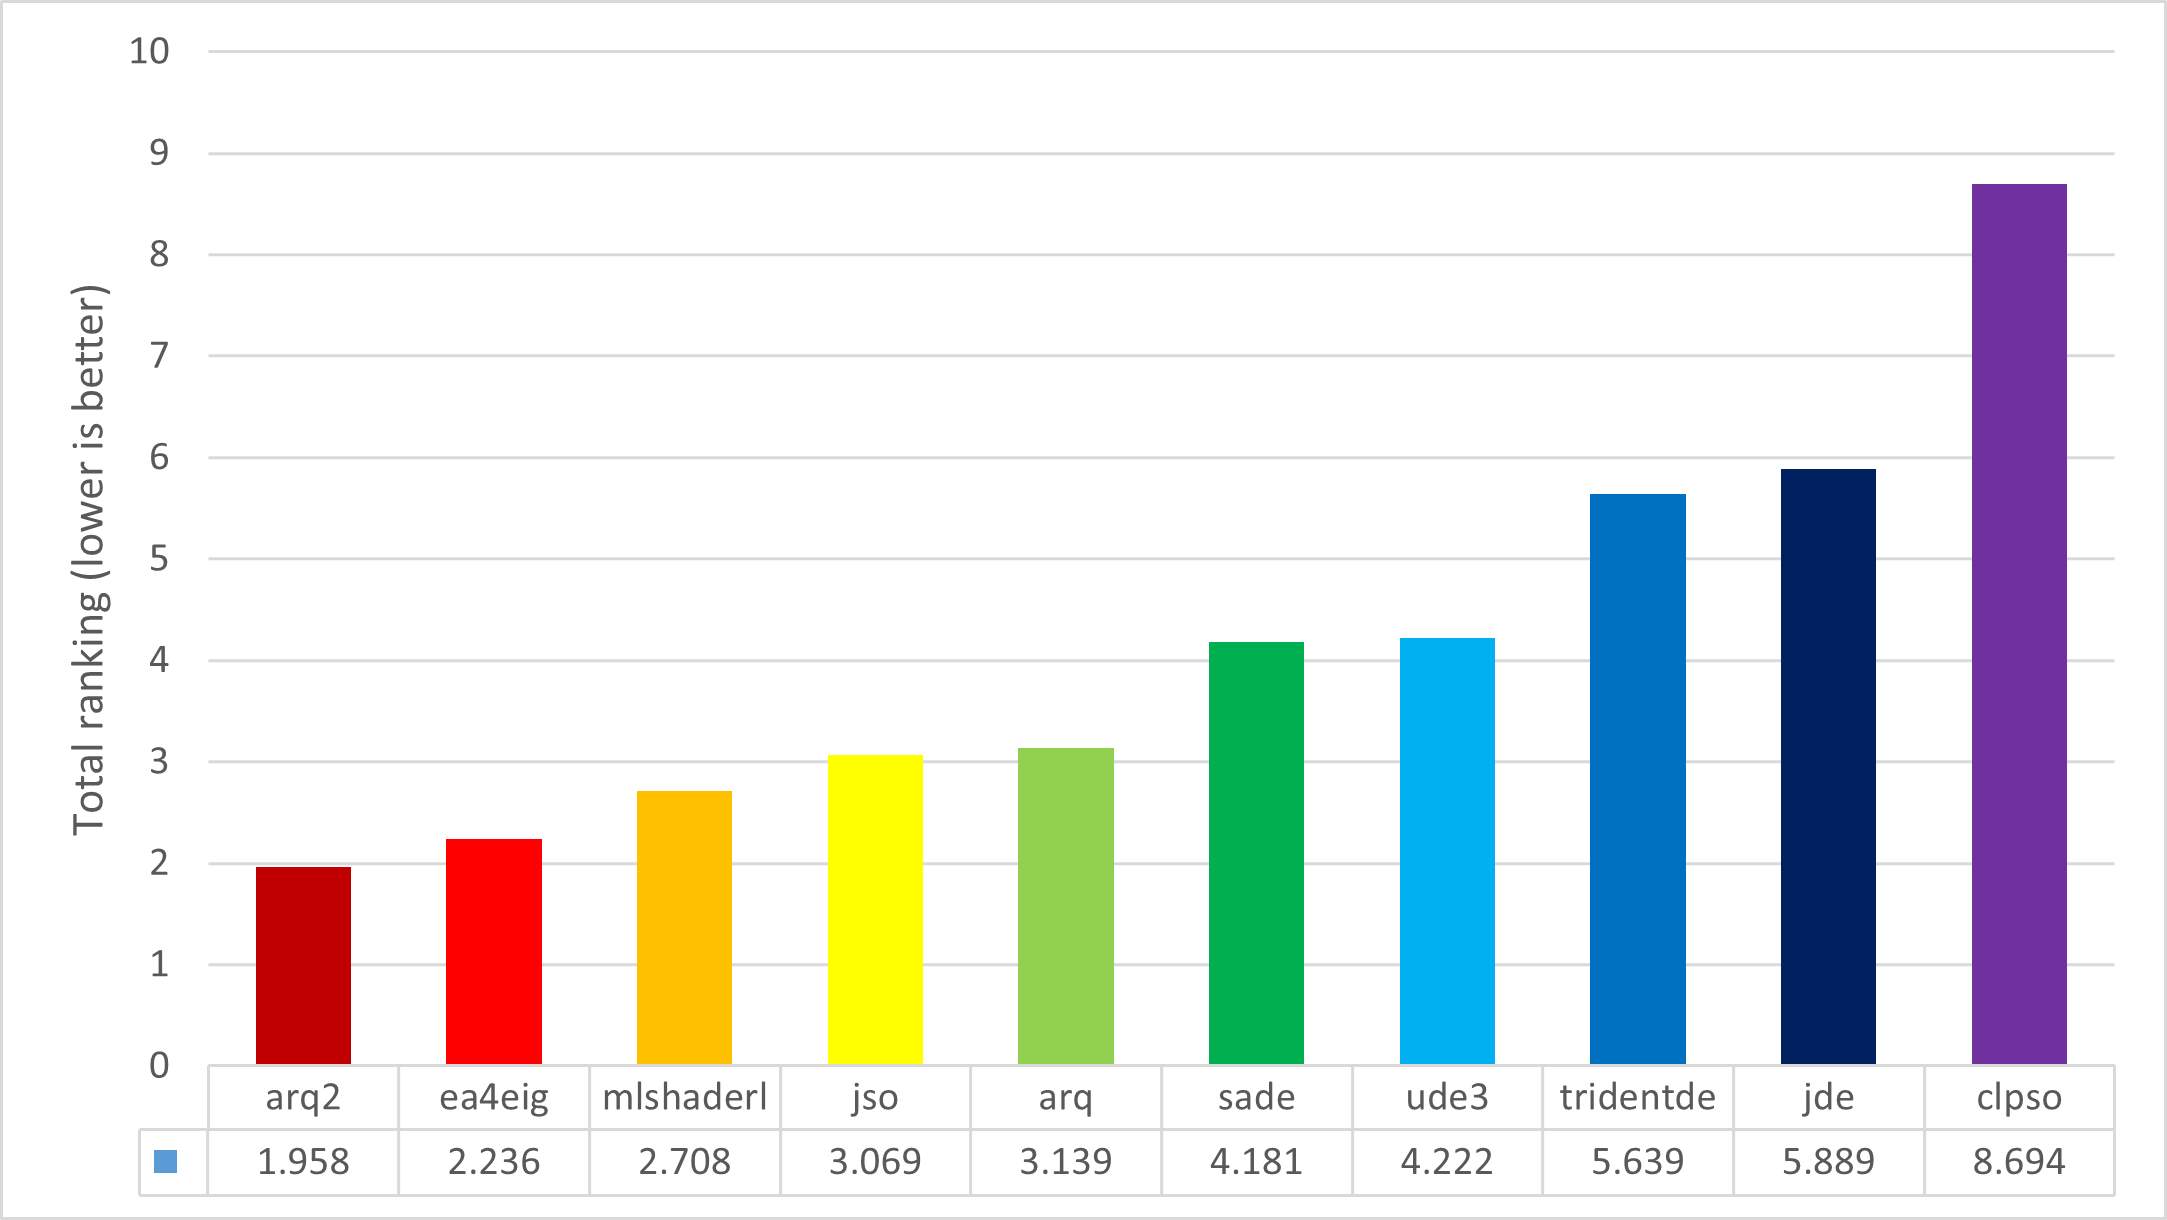
\includegraphics{totalR}
\par\end{centering}
\caption{Total ranking combining Best and Mean across 10 algorithms\label{fig:totalBarR}}

\end{figure}

Figure \ref{fig:totalBarR} provides a compact visual summary of the
overall comparative ranking of the evaluated methods, where lower
values indicate better aggregate performance. ARQ2 attains the lowest
total ranking value (1.958), followed by EA4Eig (2.236) and MLSHADE-RL
(2.708), which confirms its first overall position on the complete
benchmark suite. The figure also shows a clear separation between
the leading group of methods and the weaker-performing algorithms,
with CLPSO exhibiting the highest total ranking value. Overall, the
graphical comparison is consistent with the tabulated ranking results
and further supports the conclusion that ARQ2 achieves the most favorable
global balance among the compared optimizers.
\end{landscape}

To assess whether the performance differences reported in Tables \ref{tab:bestR}
and \ref{tab:meanR} reflect genuine statistical superiority rather
than sampling variability, pairwise Wilcoxon signed-rank tests were
conducted between ARQ2 and each competitor across all 36 benchmark
problems. Bonferroni correction was applied to the resulting p-values
to control the family-wise error rate under multiple comparisons.
The adjusted significance levels follow the standard notation: {*}{*}{*}
for p \textless{} 0.001, {*}{*} for p \textless{} 0.01, and ns for
non-significant differences. Figure \ref{fig:wilcoxonPlot} summarizes
the test outcomes for both the best-value and mean-value criteria
on a shared logarithmic scale.

\begin{figure}[H]
\raggedright
\begin{centering}
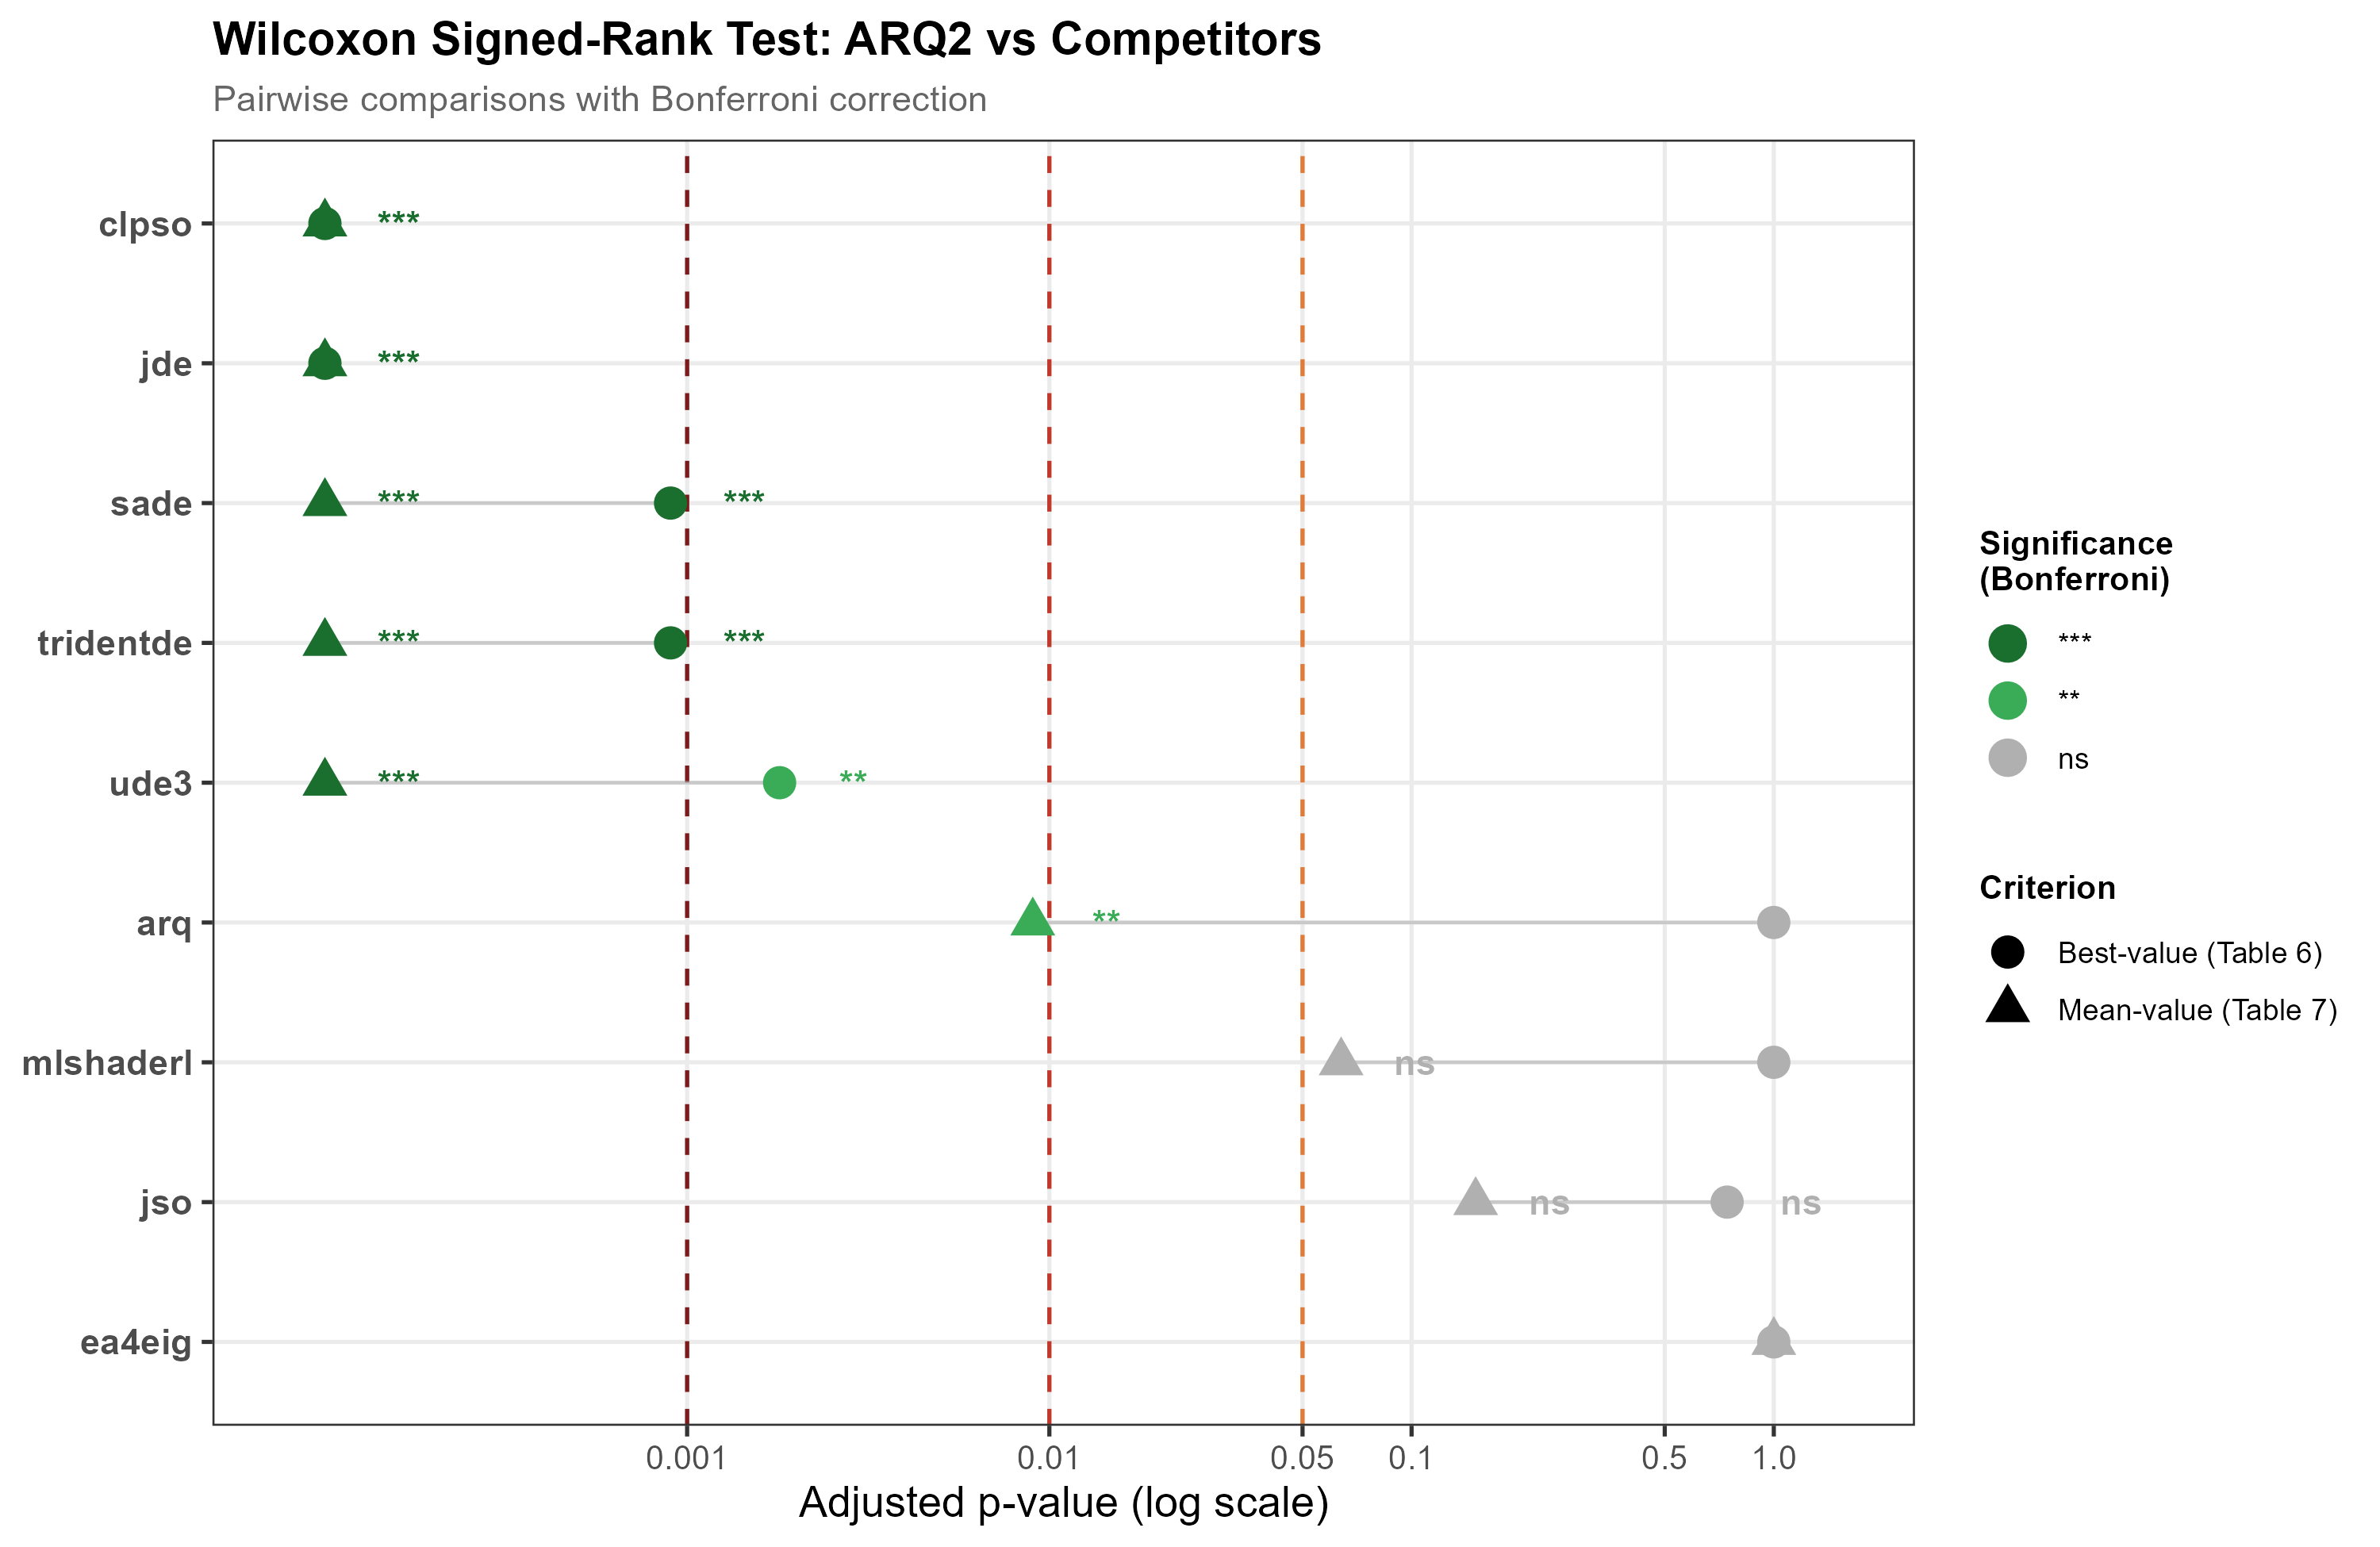
\includegraphics[scale=0.45]{wilcoxon_plot}
\par\end{centering}
\caption{Bonferroni-corrected Wilcoxon signed-rank test results: ARQ2 vs. each
competitor (best and mean criteria).\label{fig:wilcoxonPlot}}
\end{figure}

The visual evidence of Figure \ref{fig:wilcoxonPlot} is complemented
by the exact adjusted p-values reported in Table \ref{tab:wilcoxon},
which also lists the raw p-values prior to correction for completeness
and reproducibility. The table separates the best-value and mean-value
comparisons, allowing the significance pattern to be examined independently
under the two performance criteria.

\begin{table}
\caption{Bonferroni-corrected Wilcoxon signed-rank p-values: ARQ2 vs. each
competitor (best and mean criteria).\label{tab:wilcoxon}}

\centering{}{\footnotesize{}%
\begin{tabular}{|c|c|c|c|c|c|c|}
\hline 
{\footnotesize Competitor} & {\footnotesize p value best} & {\footnotesize p adjusted best} & {\footnotesize Sig. best} & {\footnotesize p value mean} & {\footnotesize p adjusted mean} & {\footnotesize Sig. mean}\tabularnewline
\hline 
\hline 
{\footnotesize clpso} & {\footnotesize 0} & {\footnotesize 0} & {\footnotesize{*}{*}{*}} & {\footnotesize 0} & {\footnotesize 0} & {\footnotesize{*}{*}{*}}\tabularnewline
\hline 
{\footnotesize jde} & {\footnotesize 0} & {\footnotesize 0} & {\footnotesize{*}{*}{*}} & {\footnotesize 0} & {\footnotesize 0} & {\footnotesize{*}{*}{*}}\tabularnewline
\hline 
{\footnotesize sade} & {\footnotesize 0.0001} & {\footnotesize 0.0009} & {\footnotesize{*}{*}{*}} & {\footnotesize 0} & {\footnotesize 0} & {\footnotesize{*}{*}{*}}\tabularnewline
\hline 
{\footnotesize tridentde} & {\footnotesize 0.0001} & {\footnotesize 0.0009} & {\footnotesize{*}{*}{*}} & {\footnotesize 0} & {\footnotesize 0} & {\footnotesize{*}{*}{*}}\tabularnewline
\hline 
{\footnotesize ude3} & {\footnotesize 0.0002} & {\footnotesize 0.0018} & {\footnotesize{*}{*}} & {\footnotesize 0} & {\footnotesize 0} & {\footnotesize{*}{*}{*}}\tabularnewline
\hline 
{\footnotesize arq} & {\footnotesize 0.5214} & {\footnotesize 1} & {\footnotesize ns} & {\footnotesize 0.001} & {\footnotesize 0.009} & {\footnotesize{*}{*}}\tabularnewline
\hline 
{\footnotesize mlshaderl} & {\footnotesize 0.1141} & {\footnotesize 1} & {\footnotesize ns} & {\footnotesize 0.0071} & {\footnotesize 0.0639} & {\footnotesize ns}\tabularnewline
\hline 
{\footnotesize jso} & {\footnotesize 0.826} & {\footnotesize 0.7434} & {\footnotesize ns} & {\footnotesize 0.0167} & {\footnotesize 0.1503} & {\footnotesize ns}\tabularnewline
\hline 
{\footnotesize ea4eig} & {\footnotesize 0.1617} & {\footnotesize 1} & {\footnotesize ns} & {\footnotesize 0.3402} & {\footnotesize 1} & {\footnotesize ns}\tabularnewline
\hline 
\end{tabular}}{\footnotesize\par}
\end{table}

The statistical results confirm that the advantage of ARQ2 over the
weaker competitors is not attributable to chance. ARQ2 is significantly
superior to CLPSO, jDE, SaDE, and TRIDENT-DE under both criteria at
the strictest significance level, and to UDE3 at the {*}{*} level
for best values and {*}{*}{*} for mean values. Against ARQ, the difference
reaches statistical significance only in mean-value terms (p-adjusted
= 0.009), which is consistent with the interpretation that ARQ2 primarily
strengthens repeated-run reliability rather than peak performance.
The comparisons with the three strongest rivals EA4Eig, JSO, and MLSHADE-RL
remain non-significant under both criteria after Bonferroni correction,
indicating that the ranking advantage of ARQ2 over these methods,
while consistent in aggregate, does not translate into a statistically
separable performance gap at the individual-problem level.

\subsection{Empirical Convergence Complexity of ARQ2\label{subsec:complexity}}

In population-based stochastic optimization, complexity is not only
associated with formal operation counts, but also with the amount
of search effort required to achieve sustained improvement under a
fixed evaluation budget. From this perspective, empirical convergence
complexity describes how effectively a method converts its available
evaluations into progressive reduction of the objective value. Its
examination is relevant because final rankings alone do not show how
rapidly or how consistently performance develops during the search
process.

Figure \ref{fig:convergenceANDcomplexity} provides this complementary
perspective through representative convergence profiles of ARQ2. The
first two problems, Ellipsoidal and Exponential, belong to the non-realworld
subset of the benchmark suite, whereas the third problem, OFDMPower,
belongs to the real-world subset. This selection makes it possible
to observe the search behavior of the proposed method on both classical
synthetic landscapes and a practical application-oriented problem.
The convergence traces appear visually thicker than a single smooth
curve because they reflect the behavior of ARQ2 over 30 independent
runs. This thickness should therefore be interpreted as an empirical
indication of run-to-run variability around the general convergence
trend rather than as a graphical artifact. Quantitatively, the width
of the convergence band at any given evaluation count corresponds
to the range between the best and worst run trajectories across the
30 independent executions, and is therefore directly related to the
standard deviation of the best-so-far objective values reported in
Table \ref{tab:arq2VSarq}. Narrower bands indicate lower standard
deviation and stronger robustness, while wider bands reflect greater
run-to-run variability.

\begin{figure}[H]
\begin{centering}
\subfloat[Ellipsoidal]{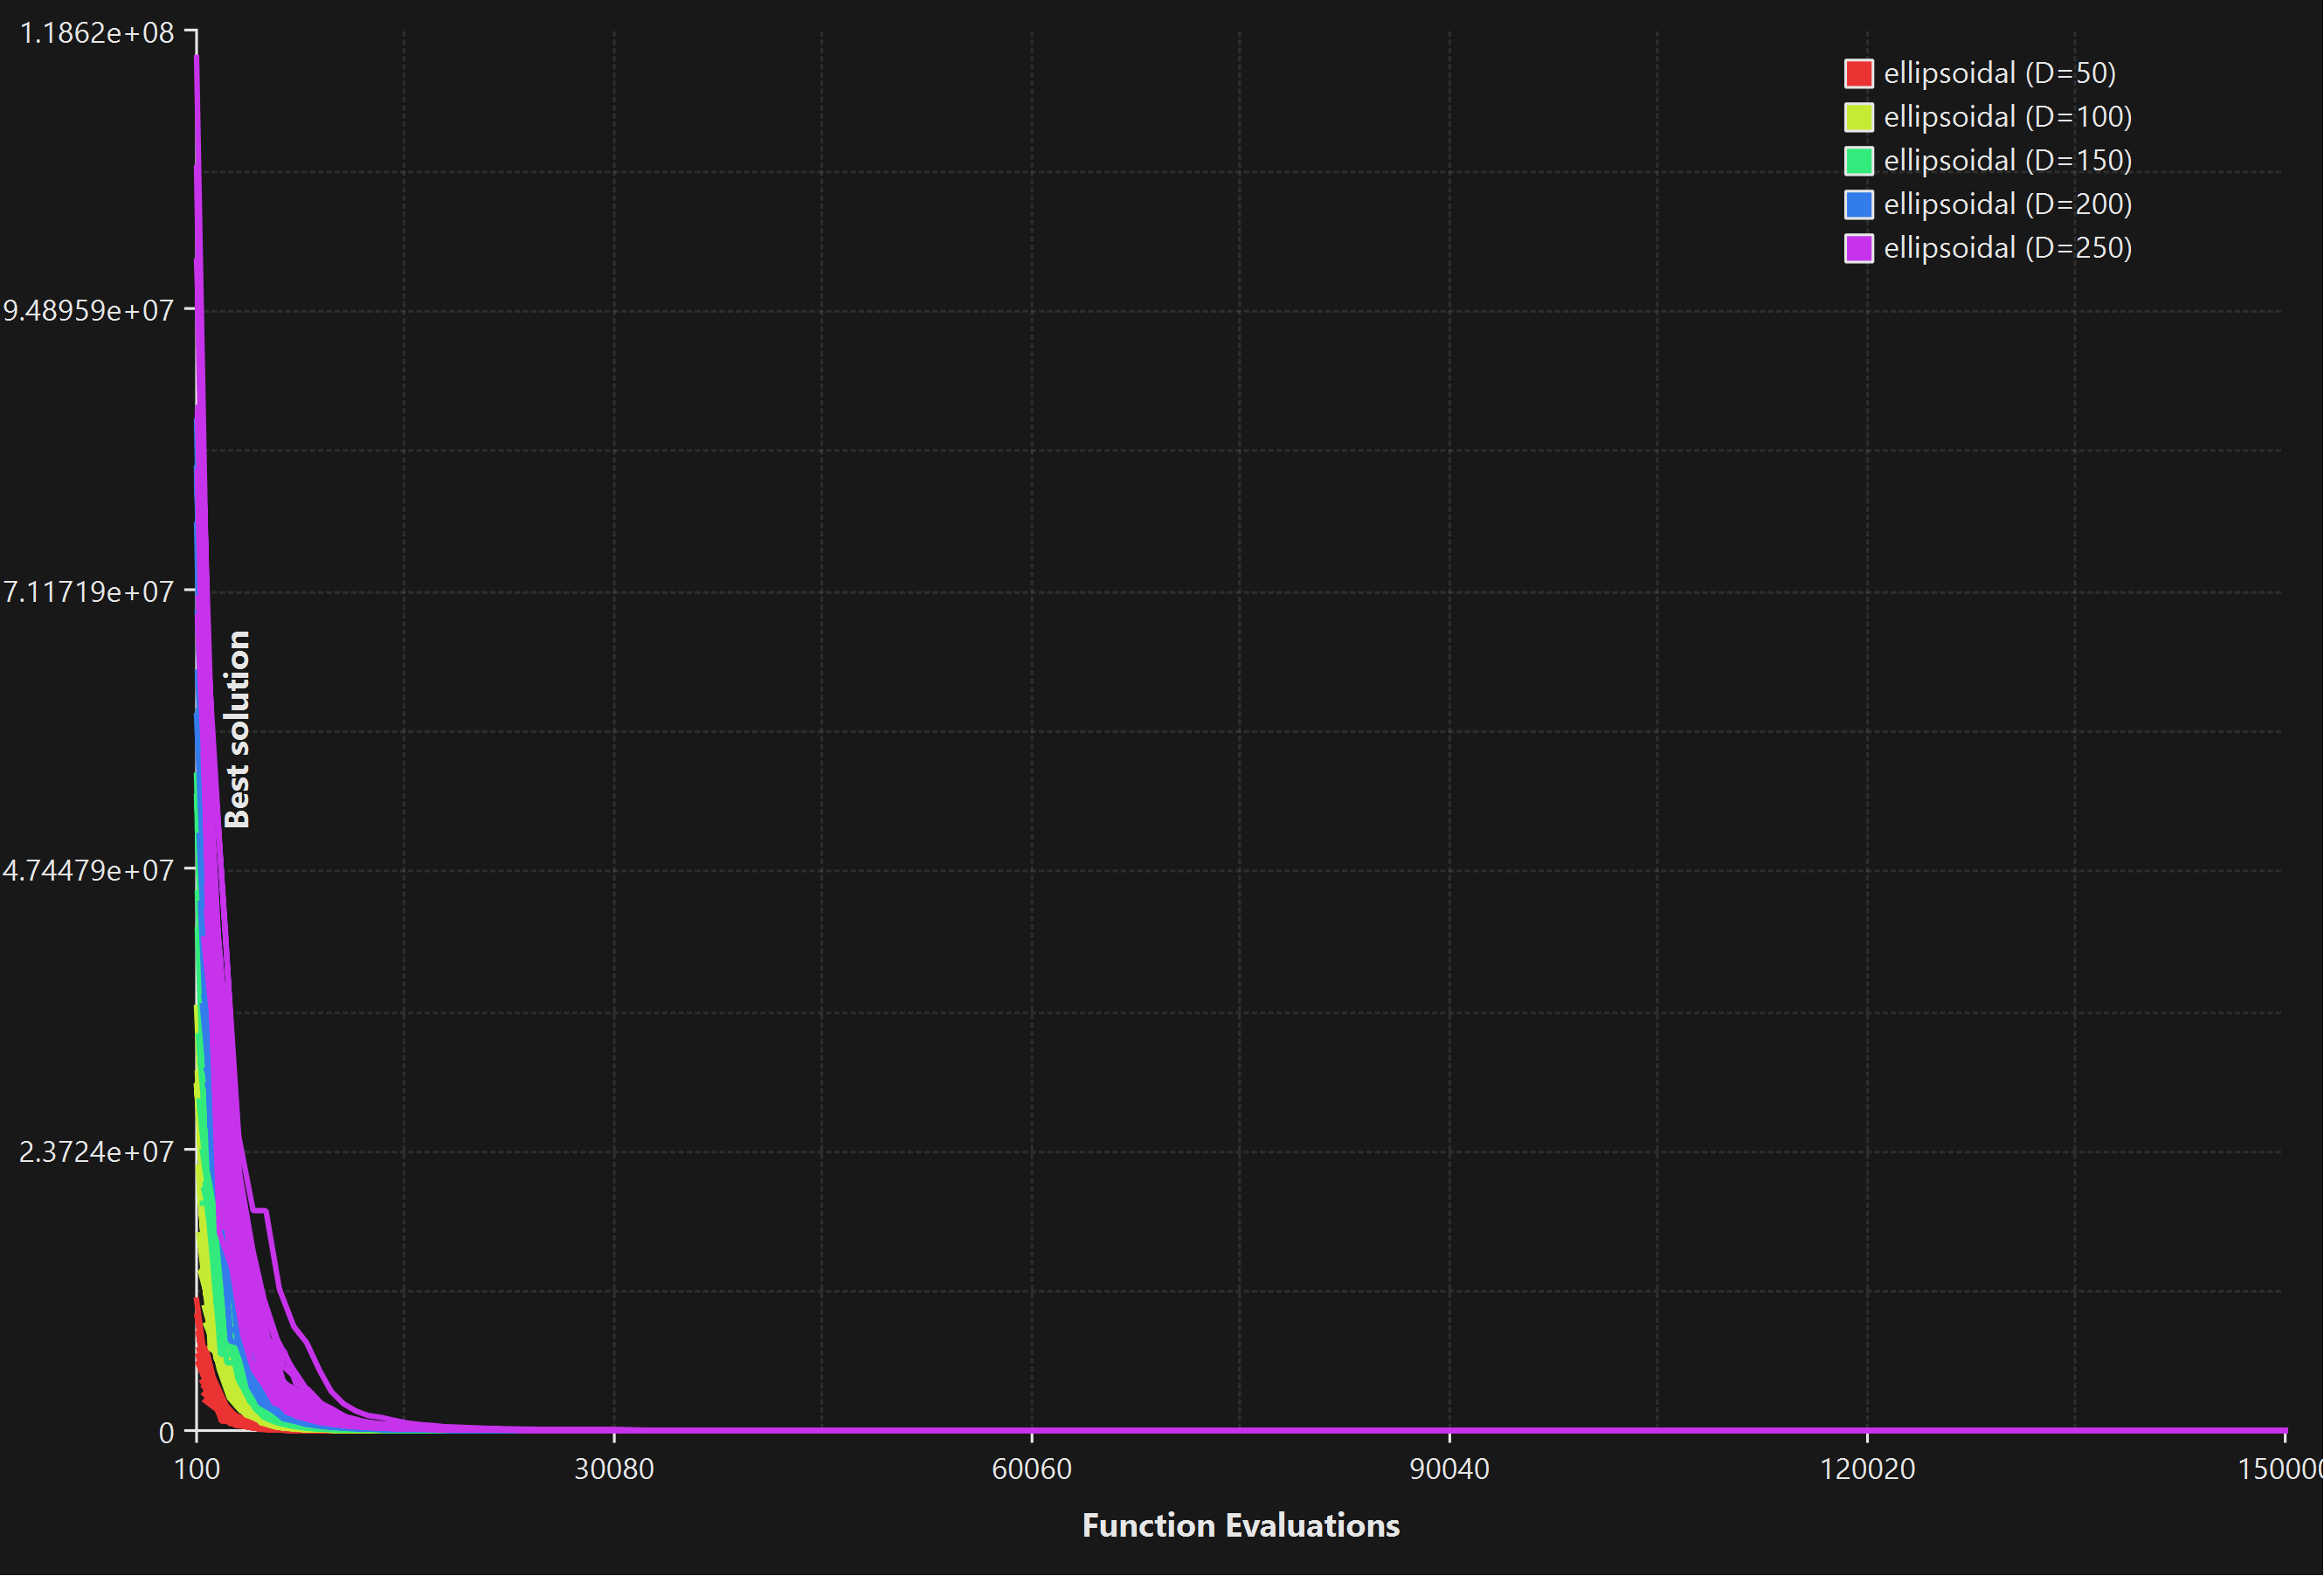
\includegraphics[scale=0.25]{arq2_ellipsoidal_convergence}

}\subfloat[Expotential]{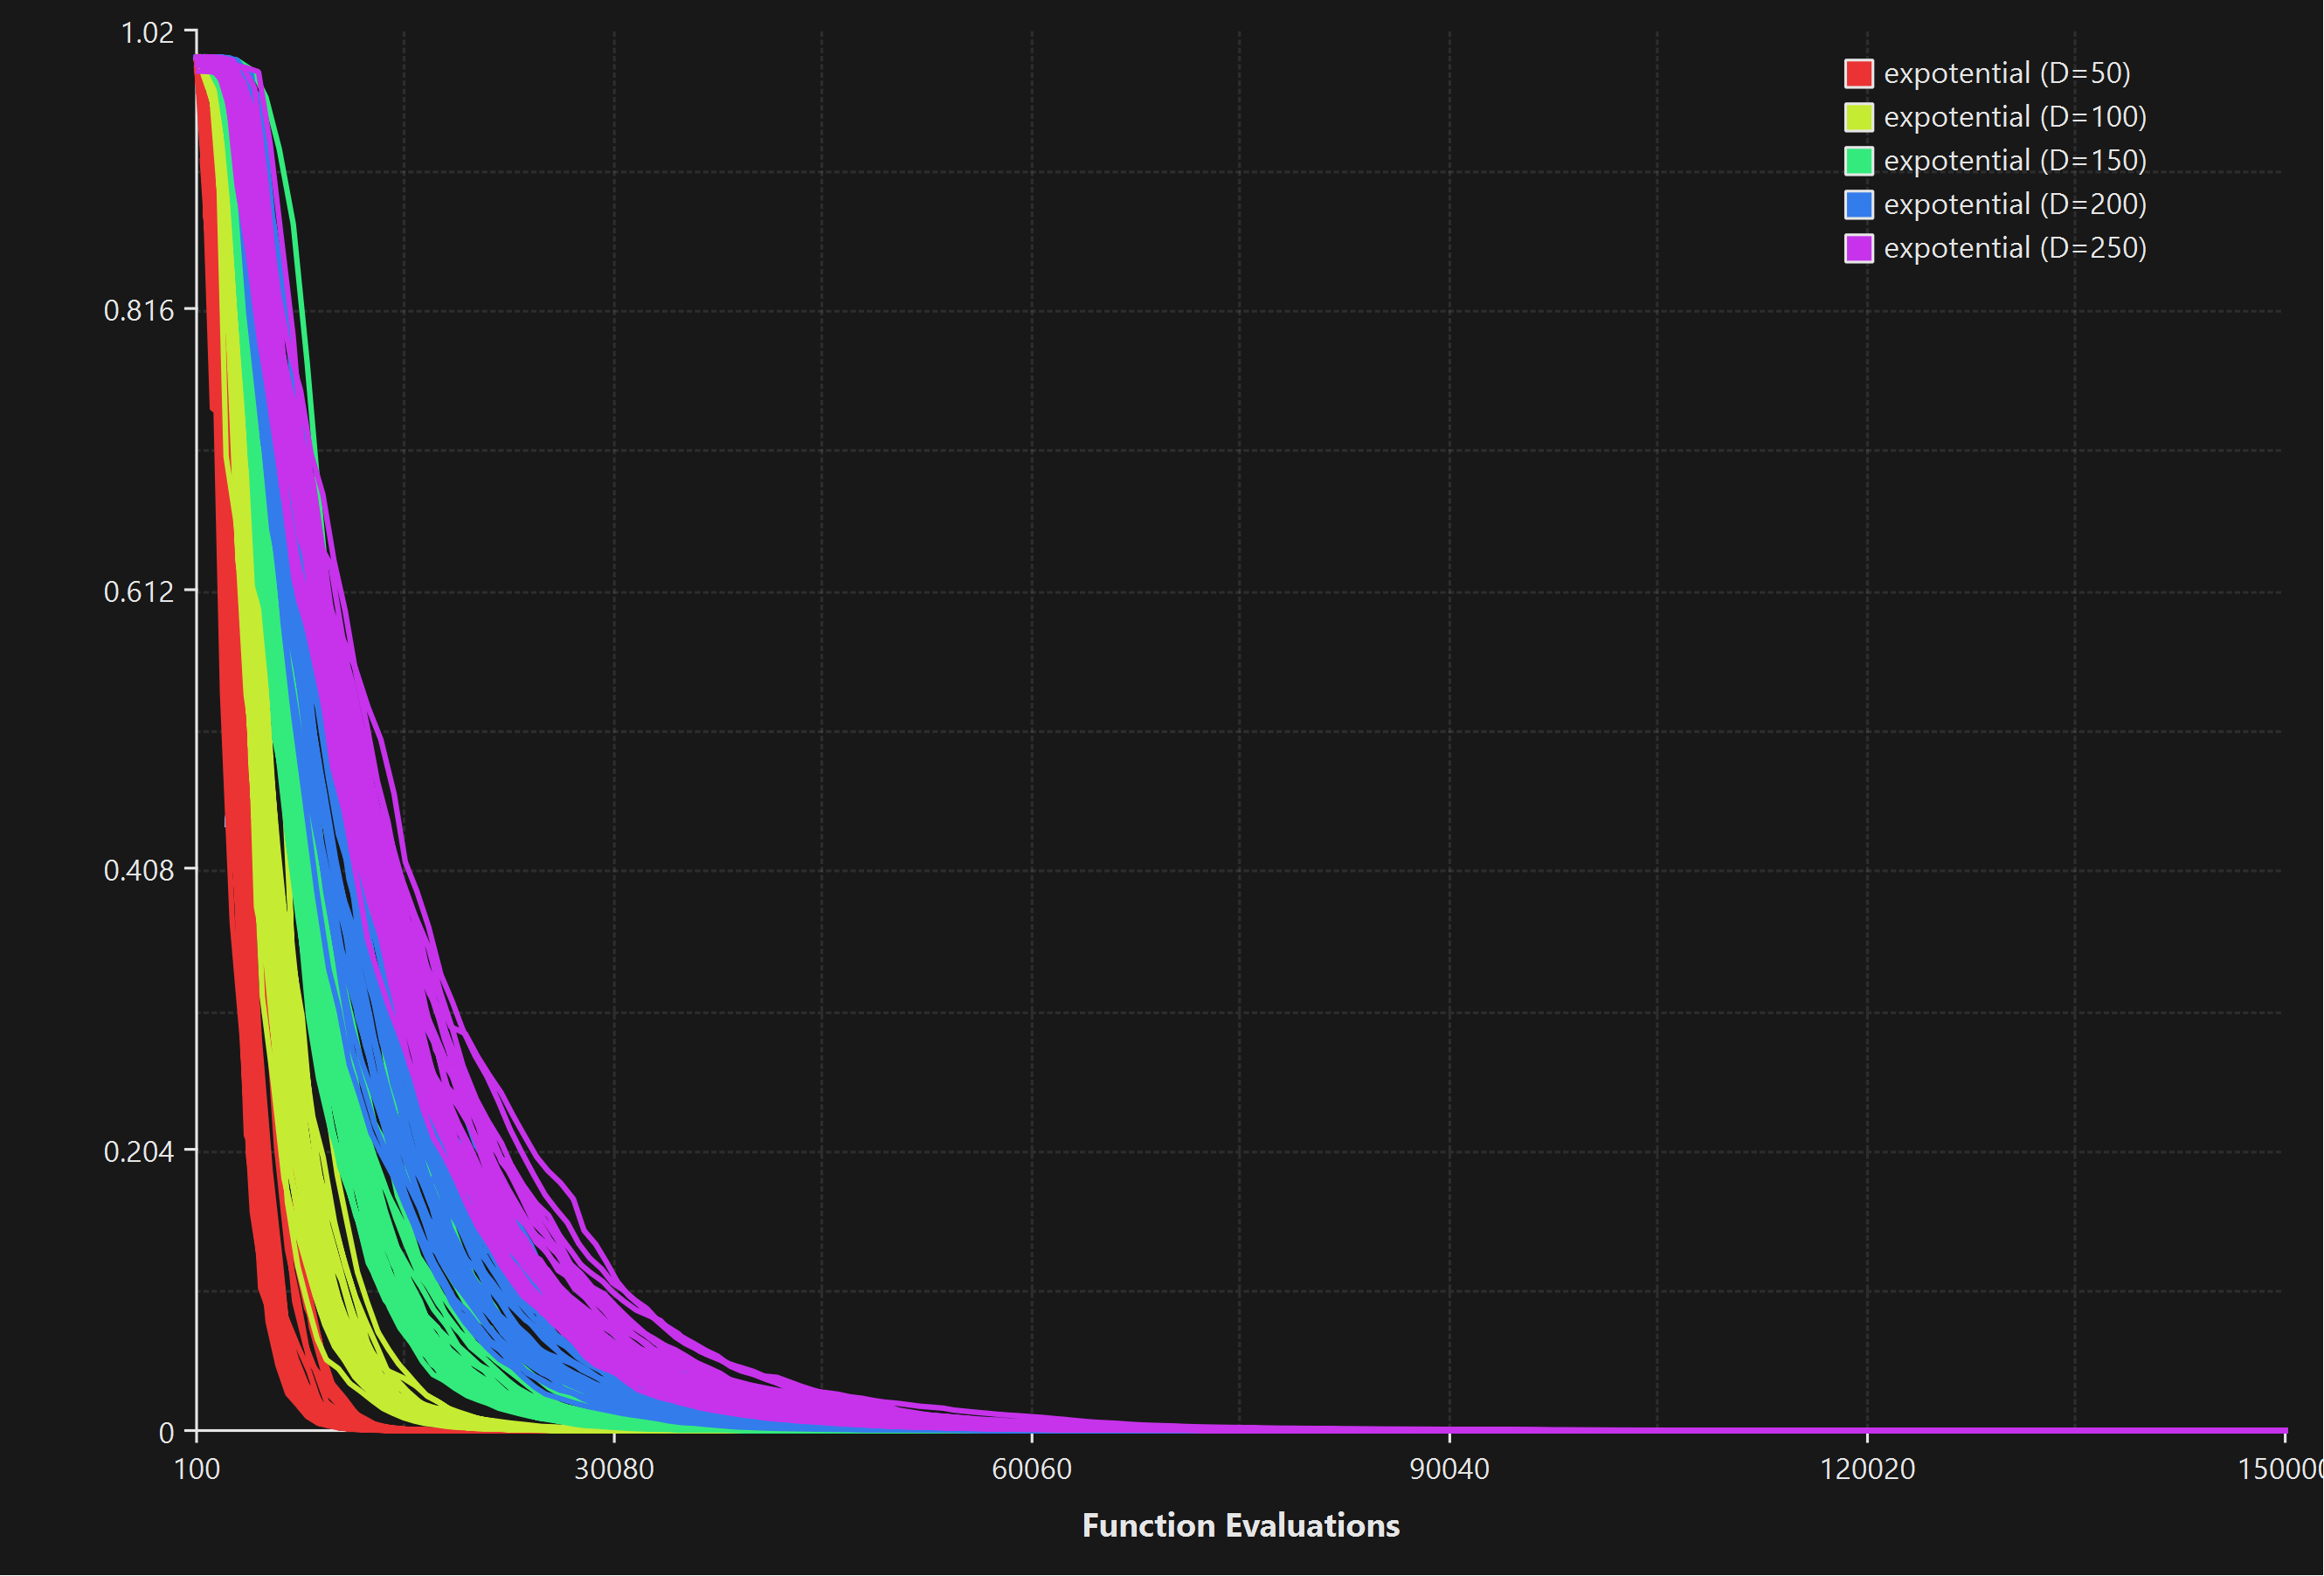
\includegraphics[scale=0.25]{arq2_expotential_convergence}

}
\par\end{centering}
\begin{centering}
\subfloat[ODFMPower]{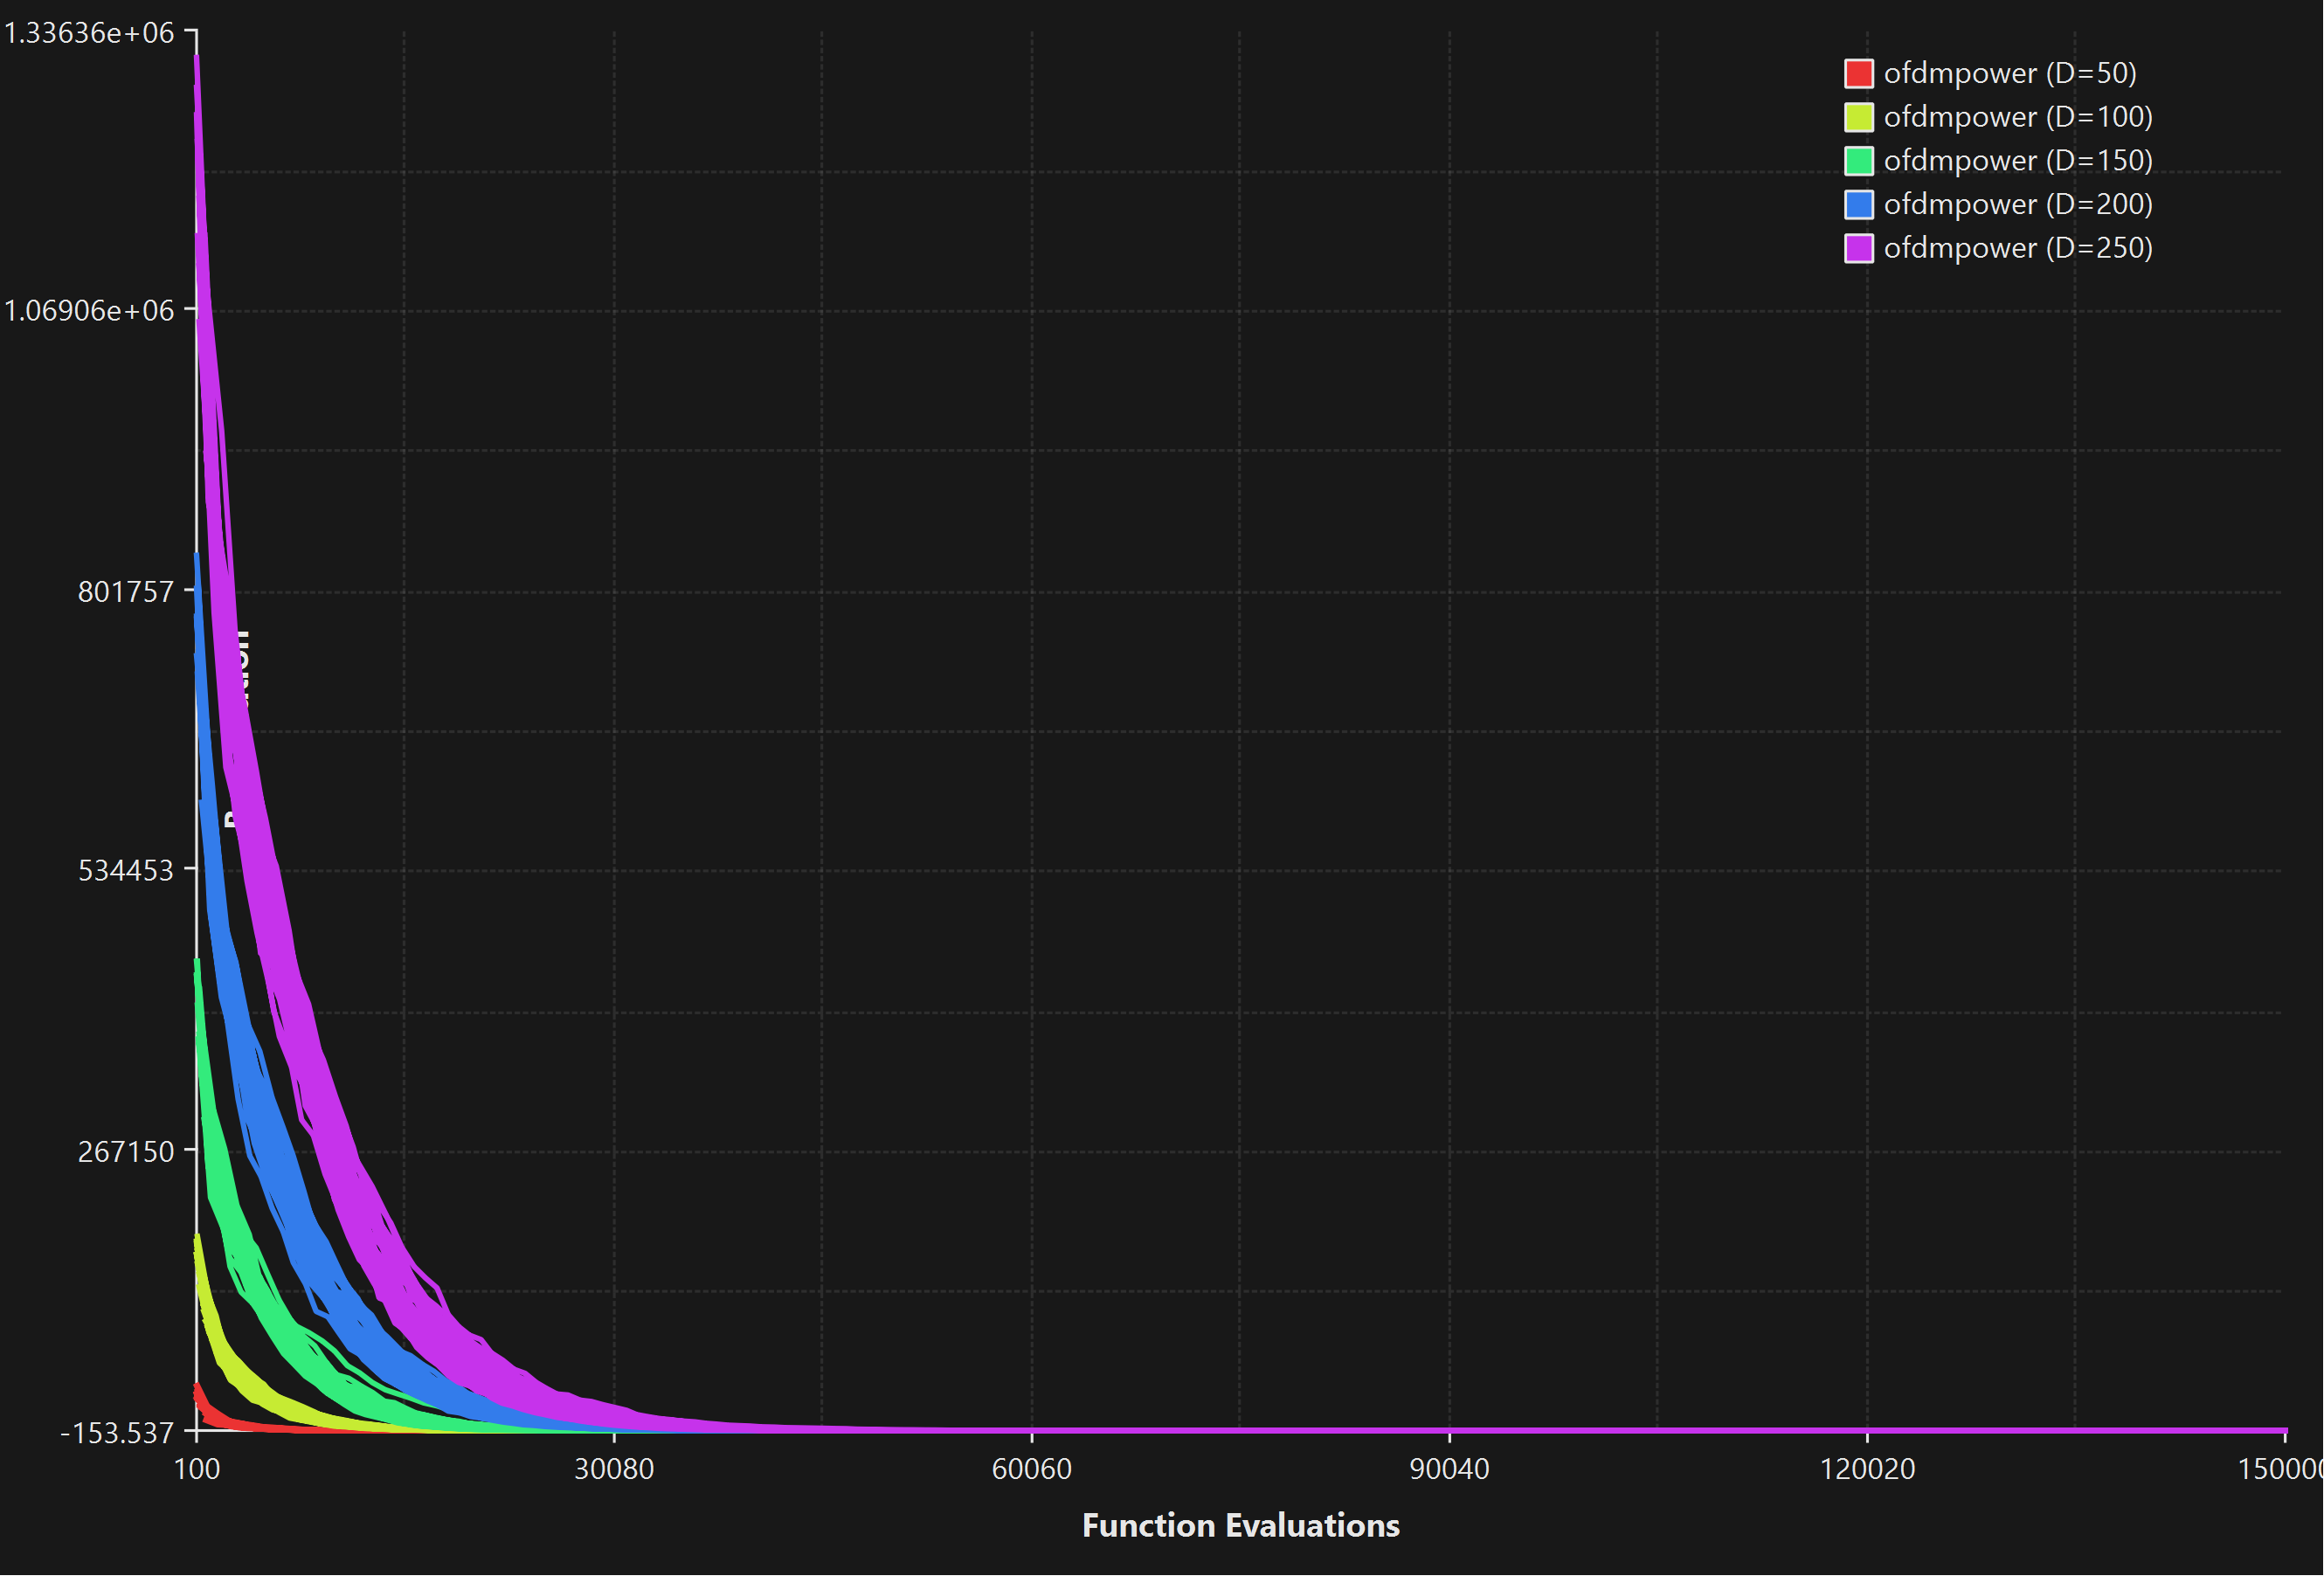
\includegraphics[scale=0.4]{arq2_ofdmpower_convergence}

}
\par\end{centering}
\caption{Empirical convergence profiles of ARQ2 over 30 independent runs on
representative benchmark problems with different landscape characteristics\label{fig:convergenceANDcomplexity}}
\end{figure}

Figure \ref{fig:convergenceANDcomplexity} provides an empirical view
of the practical convergence complexity of ARQ2 by showing how the
objective value evolves throughout the search horizon on representative
problems. In the present setting, complexity is interpreted as convergence
effort, that is, the amount of search activity required for the method
to generate consistent improvement under a fixed evaluation budget.
The plotted trajectories suggest that ARQ2 is able to reduce the objective
value progressively over a substantial portion of the optimization
process, which indicates that its hybrid search mechanisms remain
active beyond the earliest iterations and do not rely only on isolated
opportunistic improvements.

The figure also indicates that the empirical convergence complexity
of ARQ2 depends not only on the landscape type, but also on the effective
dimensional burden of the problem. As dimensionality increases, the
search space expands, the number of interacting decision components
becomes larger, and the method must coordinate exploration and refinement
in a higher-dimensional domain. For a population-based hybrid optimizer
such as ARQ2, this does not simply imply a larger formal variable
count, it also means that more search effort is typically required
before stable improvement becomes visible. From this perspective,
dimensionality contributes directly to practical optimization complexity,
because the available evaluation budget must be distributed over a
broader and more structurally demanding search domain.

This point is consistent with the contrast shown in Figure \ref{fig:convergenceANDcomplexity}.
On the two non-realworld problems, the reduction of the objective
value appears more regular and more structured, which is compatible
with smoother convergence behavior under the selected dimensional
setting. On the real-world OFDMPower problem, the descent is comparatively
slower and the convergence band is visually wider, indicating a more
demanding search process and greater variability across runs. This
difference is informative because it shows that the practical complexity
of ARQ2 is shaped jointly by landscape structure and dimensional burden
rather than by a single uniform convergence pattern over all problems.

The visual thickness of the convergence traces is itself relevant
for the interpretation of complexity. Since the figure summarizes
30 independent runs, wider bands indicate stronger dispersion of the
search trajectories and therefore a higher empirical cost for maintaining
uniform progress. Narrower bands indicate that the available search
budget is translated into more stable improvement across repeated
executions. Even under this stricter perspective, the trajectories
shown in Figure \ref{fig:convergenceANDcomplexity} remain coherent
and do not suggest abrupt instability or immediate premature stagnation.

From a methodological standpoint, Figure \ref{fig:convergenceANDcomplexity}
supports the conclusion that the additional hybridization introduced
in ARQ2 does not merely increase internal procedural complexity. Instead,
it appears to improve the way in which search effort is distributed
between exploration and refinement, even when the dimensional and
structural demands of the problem become more pronounced. The dominant
computational burden remains associated with repeated objective-function
evaluations, as is typical for population-based metaheuristics, while
the internal control mechanisms of ARQ2 contribute to a more effective
use of that evaluation budget over time. In this sense, the proposed
method exhibits a favorable empirical balance between convergence
efficiency, robustness, and practical computational demand.

\begin{figure}[H]
\centering
\begin{centering}

\includegraphics[scale=0.7]{complexity}
\par\end{centering}
\caption{Execution time of ARQ2 as a function of dimensionality on three problems\label{fig:executiontime}}
\end{figure}

Figure \ref{fig:executiontime} complements the ranking-based evidence
by showing how the execution time of ARQ2 evolves as the dimensionality
increases. A clear monotonic growth is observed for all three problems,
which indicates that the computational burden of the proposed method
increases systematically with the size of the decision space. At the
same time, the growth pattern remains relatively regular over the
tested dimensions, suggesting a stable empirical scalability profile
rather than an abrupt computational deterioration. The two non-realworld
problems, Ellipsoidal and Exponential, exhibit very similar execution-time
trajectories, with values increasing from approximately 3.95 and 4.33
seconds at dimension 50 to about 11.74 and 11.93 seconds at dimension
250. In contrast, the real-world OFDMPower problem is consistently
more demanding, increasing from 5.277 seconds at dimension 50 to 16.896
seconds at dimension 250. This difference is informative because it
shows that the practical computational complexity of ARQ2 is shaped
not only by dimensionality itself, but also by the structural characteristics
of the underlying optimization problem. Consequently, the figure supports
the view that ARQ2 maintains a regular empirical scaling trend as
dimensionality grows, while the absolute time cost becomes higher
on more demanding real-world instances.

\begin{landscape}
Table \ref{tab:times} extends the runtime analysis of Figure \ref{fig:convergenceANDcomplexity}
by reporting the mean execution time per run for all compared methods
across the complete benchmark suite. This comparison allows the computational
overhead introduced by the additional mechanisms of ARQ2 including
the dual-branch architecture, roulette scheduler, quarantine stage,
and micro-restart to be assessed directly against the baselines under
identical hardware and budget conditions.

\begin{longtable}[c]{|c|c|c|c|c|c|c|c|c|c|c|c|}
\caption{Mean execution time per run (seconds) of all compared methods on the
complete benchmark suite.\label{tab:times}}
\tabularnewline
\hline 
PROBLEM & DIM & arq2 & arq & clpso & ea4eig & jde & jso & mlshaderl & sade & tridentde & ude3\tabularnewline
\endhead
\hline 
antennaarray & 12 & 4.069 & 4.411 & 4.455 & 4.358 & 4.132 & 4.406 & 4.065 & 4.486 & 4.428 & 4.397\tabularnewline
\hline 
antennaula & 10 & 9.877 & 8.714 & 9.927 & 8.873 & 8.716 & 8.671 & 8.695 & 8.76 & 8.683 & 8.681\tabularnewline
\hline 
bifunctionalcatalyst & 1 & 0.582 & 0.596 & 0.578 & 0.552 & 0.587 & 0.555 & 0.583 & 0.64 & 0.561 & 0.554\tabularnewline
\hline 
ded1 & 120 & 0.269 & 0.192 & 0.293 & 0.194 & 0.305 & 0.204 & 0.308 & 0.233 & 0.166 & 0.151\tabularnewline
\hline 
ded2 & 216 & 0.547 & 0.497 & 0.574 & 0.603 & 0.583 & 0.62 & 0.546 & 0.469 & 0.411 & 0.371\tabularnewline
\hline 
eld1 & 6 & 0.072 & 0.07 & 0.068 & 0.028 & 0.066 & 0.031 & 0.053 & 0.12 & 0.036 & 0.028\tabularnewline
\hline 
eld2 & 13 & 0.093 & 0.089 & 0.095 & 0.044 & 0.084 & 0.048 & 0.063 & 0.141 & 0.054 & 0.043\tabularnewline
\hline 
eld3 & 15 & 0.104 & 0.095 & 0.109 & 0.052 & 0.097 & 0.057 & 0.079 & 0.149 & 0.062 & 0.051\tabularnewline
\hline 
eld4 & 40 & 0.187 & 0.141 & 0.196 & 0.097 & 0.171 & 0.1 & 0.141 & 0.201 & 0.103 & 0.093\tabularnewline
\hline 
eld5 & 140 & 0.358 & 0.204 & 0.397 & 0.189 & 0.631 & 0.207 & 0.811 & 0.255 & 0.172 & 0.15\tabularnewline
\hline 
gascycle & 4 & 0.06 & 0.068 & 0.051 & 0.022 & 0.061 & 0.025 & 0.063 & 0.118 & 0.031 & 0.022\tabularnewline
\hline 
hydrothermal & 96 & 0.325 & 0.193 & 0.362 & 0.174 & 0.659 & 0.189 & 0.953 & 0.251 & 0.163 & 0.141\tabularnewline
\hline 
ik6dof & 6 & 0.087 & 0.087 & 0.092 & 0.047 & 0.079 & 0.05 & 0.063 & 0.138 & 0.054 & 0.047\tabularnewline
\hline 
messenger & 26 & 0.083 & 0.076 & 0.085 & 0.031 & 0.08 & 0.038 & 0.078 & 0.13 & 0.043 & 0.033\tabularnewline
\hline 
ofdmpower  & 24 & 0.119 & 0.097 & 0.126 & 0.053 & 0.093 & 0.06 & 0.08 & 0.154 & 0.064 & 0.055\tabularnewline
\hline 
polyphase & 20 & 0.284 & 0.269 & 0.28 & 0.256 & 0.274 & 0.285 & 0.243 & 0.291 & 0.289 & 0.157\tabularnewline
\hline 
potential & 38 & 0.534 & 0.448 & 0.633 & 0.407 & 0.803 & 0.413 & 2.113 & 0.541 & 0.412 & 0.368\tabularnewline
\hline 
portfoliomv & 10 & 0.074 & 0.071 & 0.075 & 0.03 & 0.064 & 0.036 & 0.05 & 0.124 & 0.038 & 0.039\tabularnewline
\hline 
tandem & 18 & 0.092 & 0.079 & 0.096 & 0.036 & 0.101 & 0.046 & 0.095 & 0.133 & 0.048 & 0.046\tabularnewline
\hline 
tersoffb & 24 & 1.226 & 1.238 & 1.218 & 1.075 & 1.192 & 0.918 & 1.401 & 1.168 & 1.002 & 0.995\tabularnewline
\hline 
tersoffc & 24 & 1.586 & 1.503 & 1.591 & 1.238 & 1.391 & 1.062 & 1.675 & 1.387 & 1.206 & 1.245\tabularnewline
\hline 
transmissionpricing & 126 & 3.147 & 2.948 & 3.092 & 2.541 & 3.34 & 2.79 & 3.054 & 3.014 & 2.961 & 2.667\tabularnewline
\hline 
vibratingplatform & 5 & 0.069 & 0.069 & 0.07 & 0.025 & 0.063 & 0.029 & 0.058 & 0.118 & 0.034 & 0.032\tabularnewline
\hline 
wirelesscoverage & 6 & 7.161 & 6.808 & 7.34 & 7.014 & 7.279 & 7.002 & 7.218 & 7.195 & 7.023 & 6.592\tabularnewline
\hline 
bucherastrigin & 50 & 0.182 & 0.201 & 0.12 & 0.159 & 0.131 & 0.122 & 0.194 & 0.125 & 0.095 & 0.152\tabularnewline
\hline 
gallagher101 & 10 & 0.535 & 0.536 & 0.492 & 0.525 & 0.5 & 0.511 & 0.579 & 0.502 & 0.492 & 0.535\tabularnewline
\hline 
gallagher21 & 10 & 0.175 & 0.216 & 0.133 & 0.166 & 0.137 & 0.149 & 0.257 & 0.16 & 0.147 & 0.214\tabularnewline
\hline 
levy & 24 & 0.127 & 0.129 & 0.064 & 0.093 & 0.066 & 0.076 & 0.166 & 0.07 & 0.064 & 0.102\tabularnewline
\hline 
lunacekbirastrigin & 40 & 0.176 & 0.205 & 0.099 & 0.15 & 0.111 & 0.119 & 0.196 & 0.103 & 0.098 & 0.157\tabularnewline
\hline 
rotatedrosenbrock & 50 & 0.16 & 0.165 & 0.069 & 0.103 & 0.076 & 0.085 & 0.178 & 0.077 & 0.071 & 0.11\tabularnewline
\hline 
schaffer & 2 & 0.057 & 0.052 & 0.017 & 0.053 & 0.021 & 0.038 & 0.108 & 0.026 & 0.034 & 0.062\tabularnewline
\hline 
schwefel & 16 & 0.094 & 0.111 & 0.045 & 0.085 & 0.053 & 0.097 & 0.153 & 0.057 & 0.049 & 0.112\tabularnewline
\hline 
sinusoidal & 100 & 0.425 & 0.409 & 0.339 & 0.283 & 0.273 & 0.255 & 0.33 & 0.263 & 0.23 & 0.306\tabularnewline
\hline 
sinusoidal & 150 & 0.554 & 0.564 & 0.524 & 0.452 & 0.395 & 0.387 & 0.475 & 0.396 & 0.334 & 0.426\tabularnewline
\hline 
test2n & 200 & 0.485 & 0.372 & 0.294 & 0.66 & 0.265 & 0.453 & 0.357 & 0.255 & 0.173 & 0.246\tabularnewline
\hline 
weierstrass & 50 & 4.324 & 4.309 & 4.908 & 4.437 & 4.624 & 4.264 & 4.301 & 4.468 & 4.483 & 4.431\tabularnewline
\hline 
Total &  & 38.299 & 36.232 & 38.907 & 35.105 & 37.503 & 34.398 & 39.782 & 36.718 & 34.314 & 33.811\tabularnewline
\hline 
\end{longtable}

The results show that ARQ2 operates within a runtime range that is
broadly comparable to the other methods across the majority of benchmark
problems. The total accumulated time over all 36 problems amounts
to 38.30 seconds for ARQ2, which is higher than the leanest competitors
such as UDE3 (33.81 s) and TRIDENT-DE (34.31 s), but lower than MLSHADE-RL
(39.78 s) and close to CLPSO (38.91 s). The overhead introduced by
the additional control mechanisms of ARQ2 is therefore modest in absolute
terms and does not represent a disproportionate computational cost
relative to the performance gains documented in Tables \ref{tab:bestR},
\ref{tab:meanR}, and \ref{tab:finalR}.
\end{landscape}


\subsection{Parameter sensitivity analysis of ARQ2\label{subsec:sensitivity} }

To assess the robustness of ARQ2 with respect to its control parameters,
a systematic sensitivity analysis was conducted on three parameters
that govern the core behavioral mechanisms of the method: the bootstrap
length b, which determines the number of ARQ-only iterations enforced
before competitive branch selection begins; the reset threshold $\delta$,
which controls the frequency of credit resets in the roulette scheduler;
and the stagnation trigger $\tau$, which sets the number of consecutive
non-improving ARQ iterations required to activate the micro-restart
mechanism. Each parameter was varied across five levels while the
remaining parameters were held at their default values, as reported
in Table 1. The analysis was performed on three representative benchmark
problems that cover complementary problem characteristics: test2n
(D=200), a high-dimensional separable function; tersoffc (D=24), a
real-world molecular potential with a complex multimodal landscape;
and weierstrass (D=50), a highly multimodal function with a fractal-like
structure. Mean best-value performance over 30 independent runs is
reported in each case. The results are summarized in Figures \ref{fig:test2n200},
\ref{fig:tersoffc}, and \ref{fig:weiresrtrass50}.

\begin{figure}[H]
\centering{}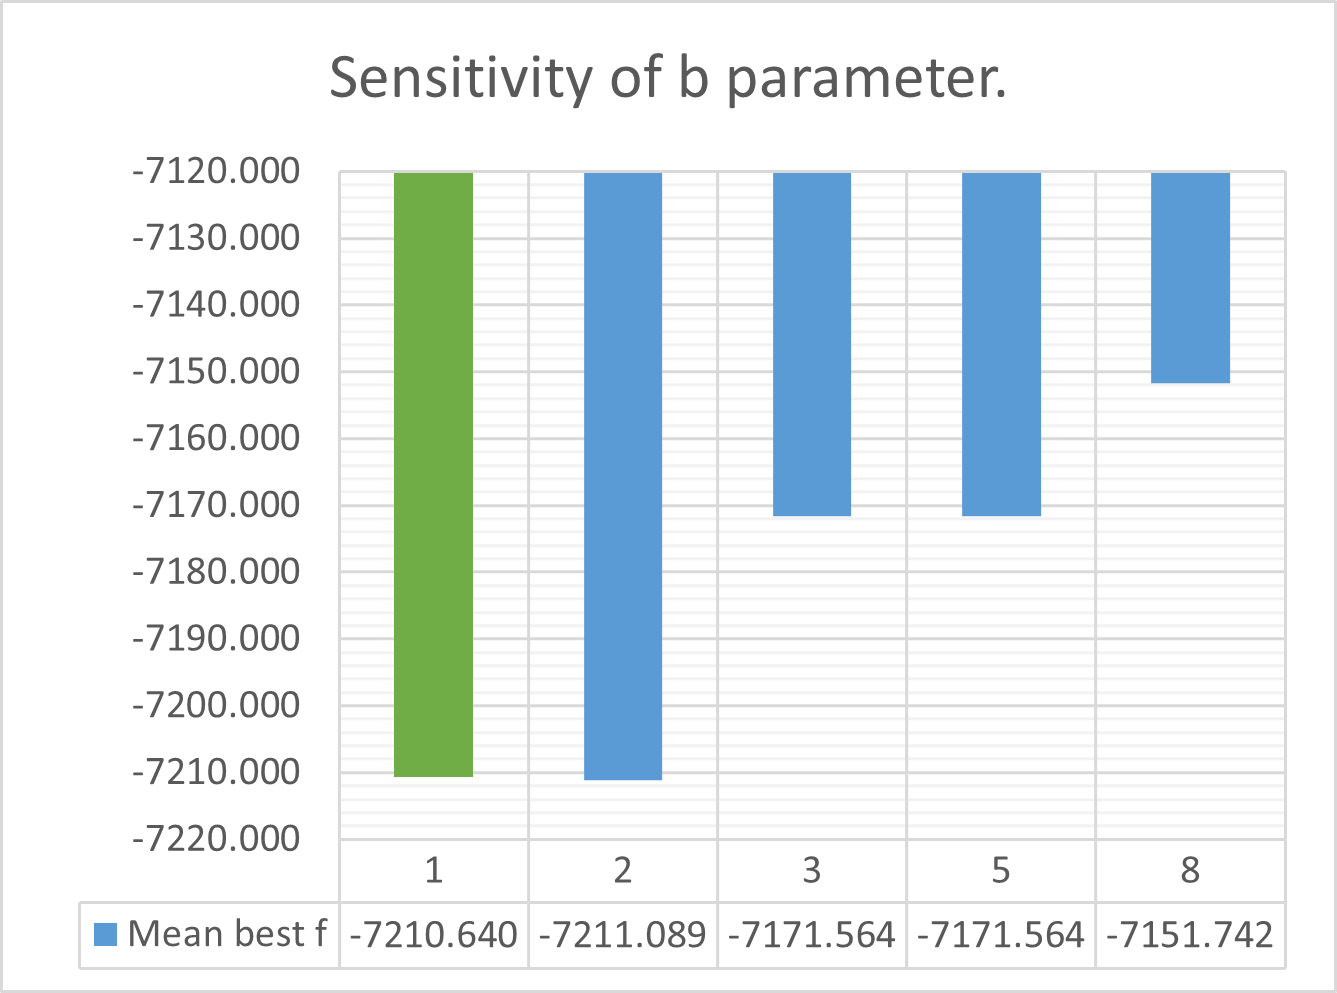
\includegraphics[scale=0.45]{test2n200_b}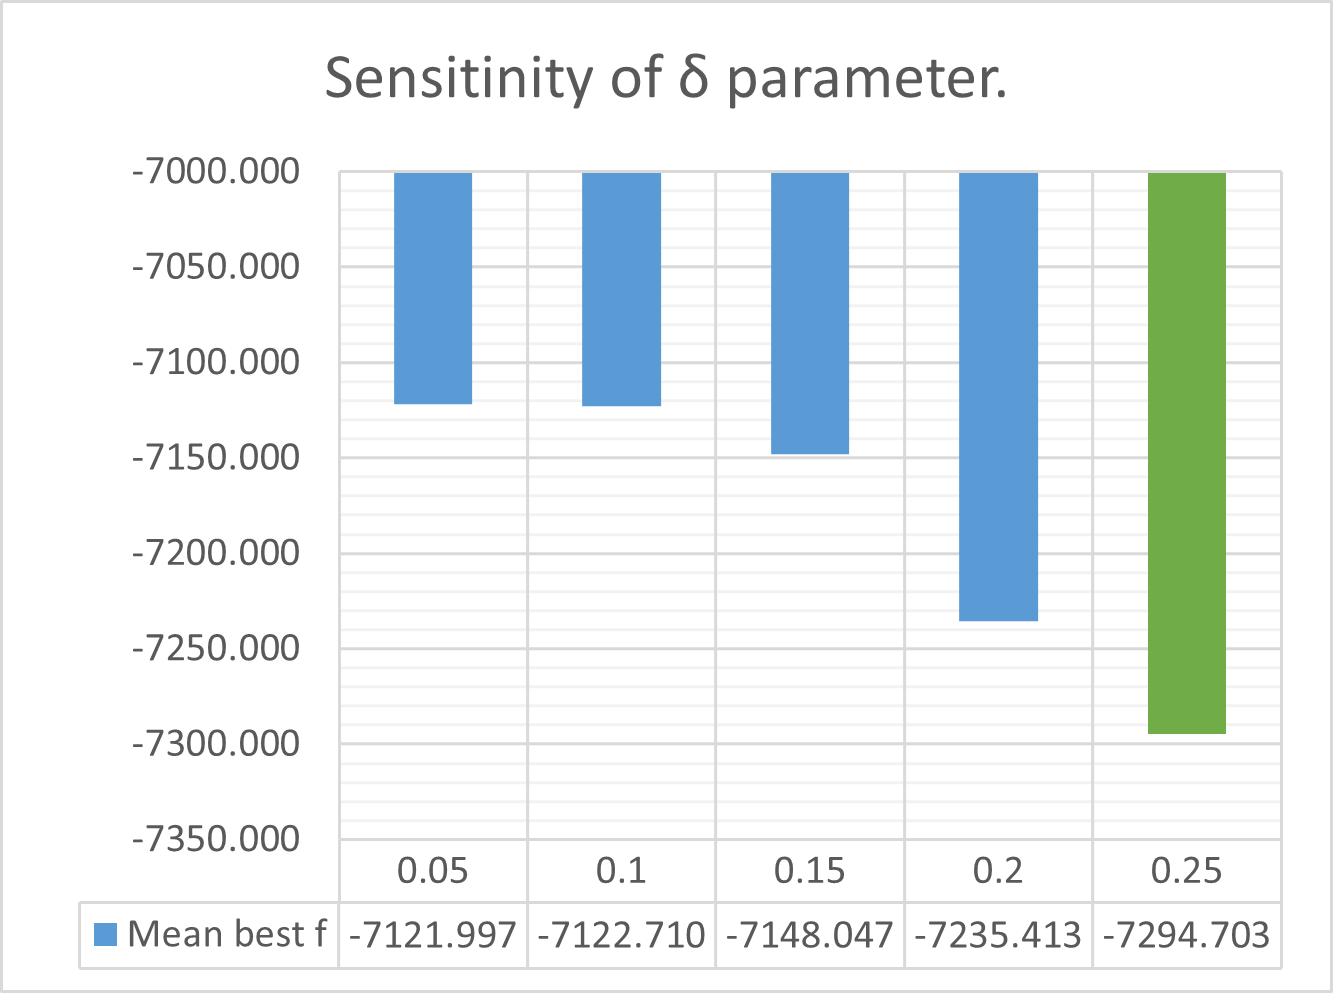
\includegraphics[scale=0.45]{test2n200_d}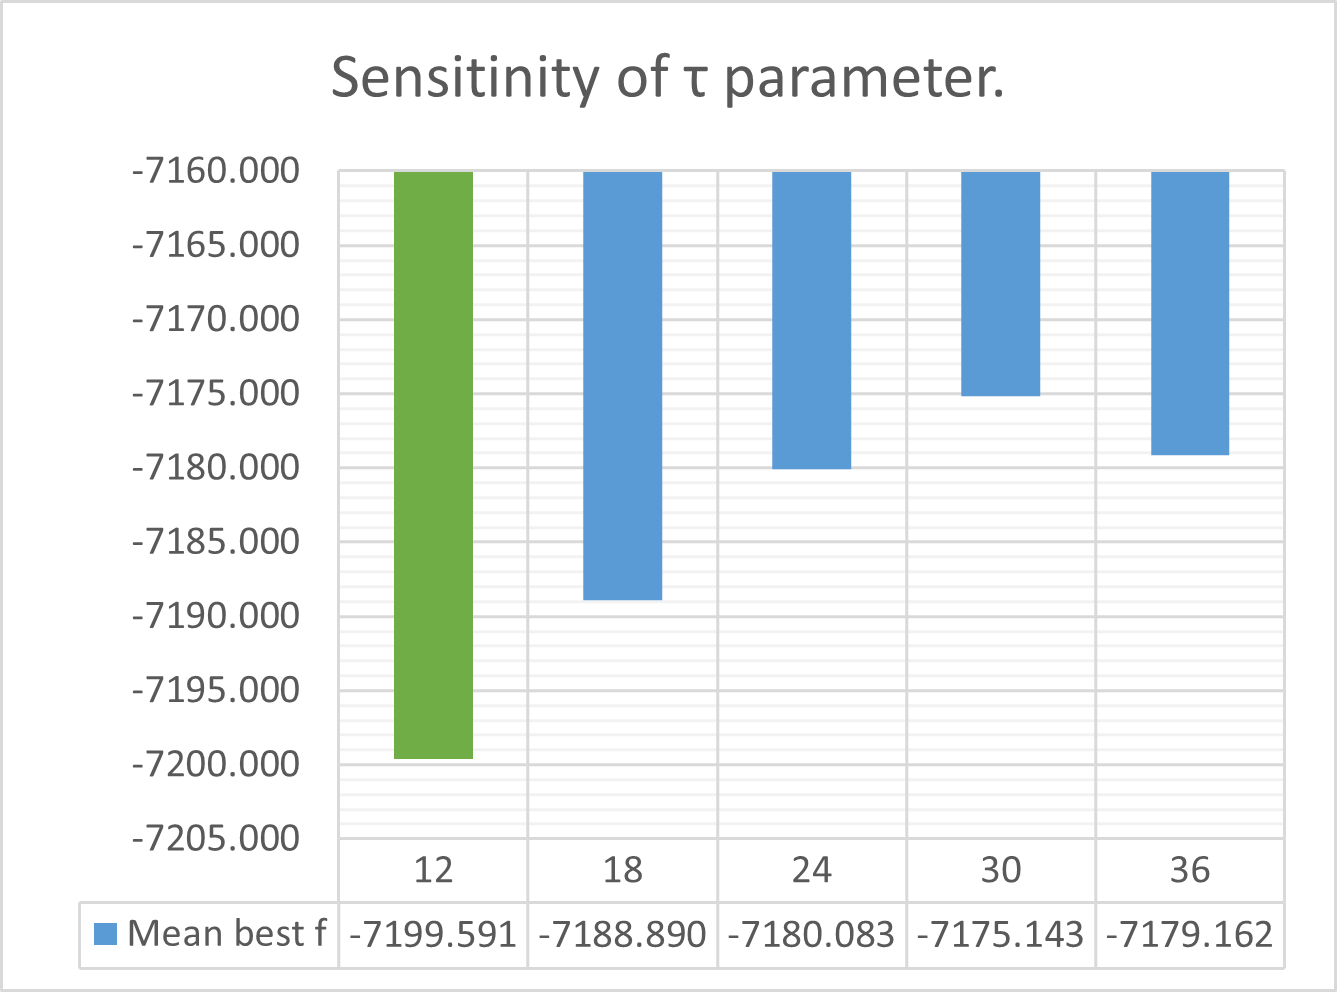
\includegraphics[scale=0.45]{test2n200_t}\caption{Test2n problem. Dimension 200.\label{fig:test2n200}}
\end{figure}
\begin{figure}[H]
\begin{centering}
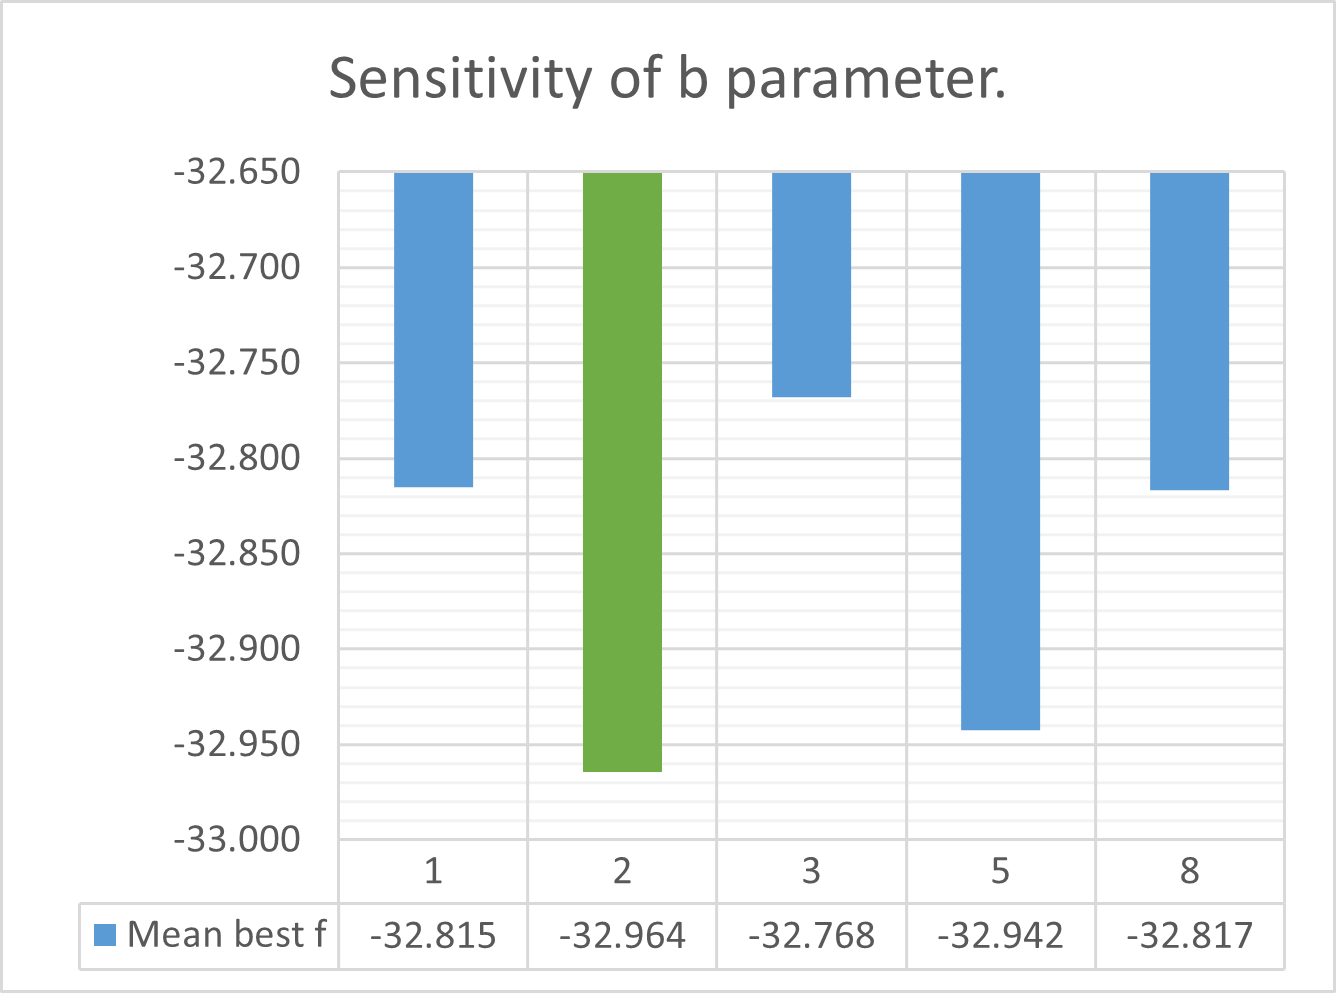
\includegraphics[scale=0.45]{tersoffc_b}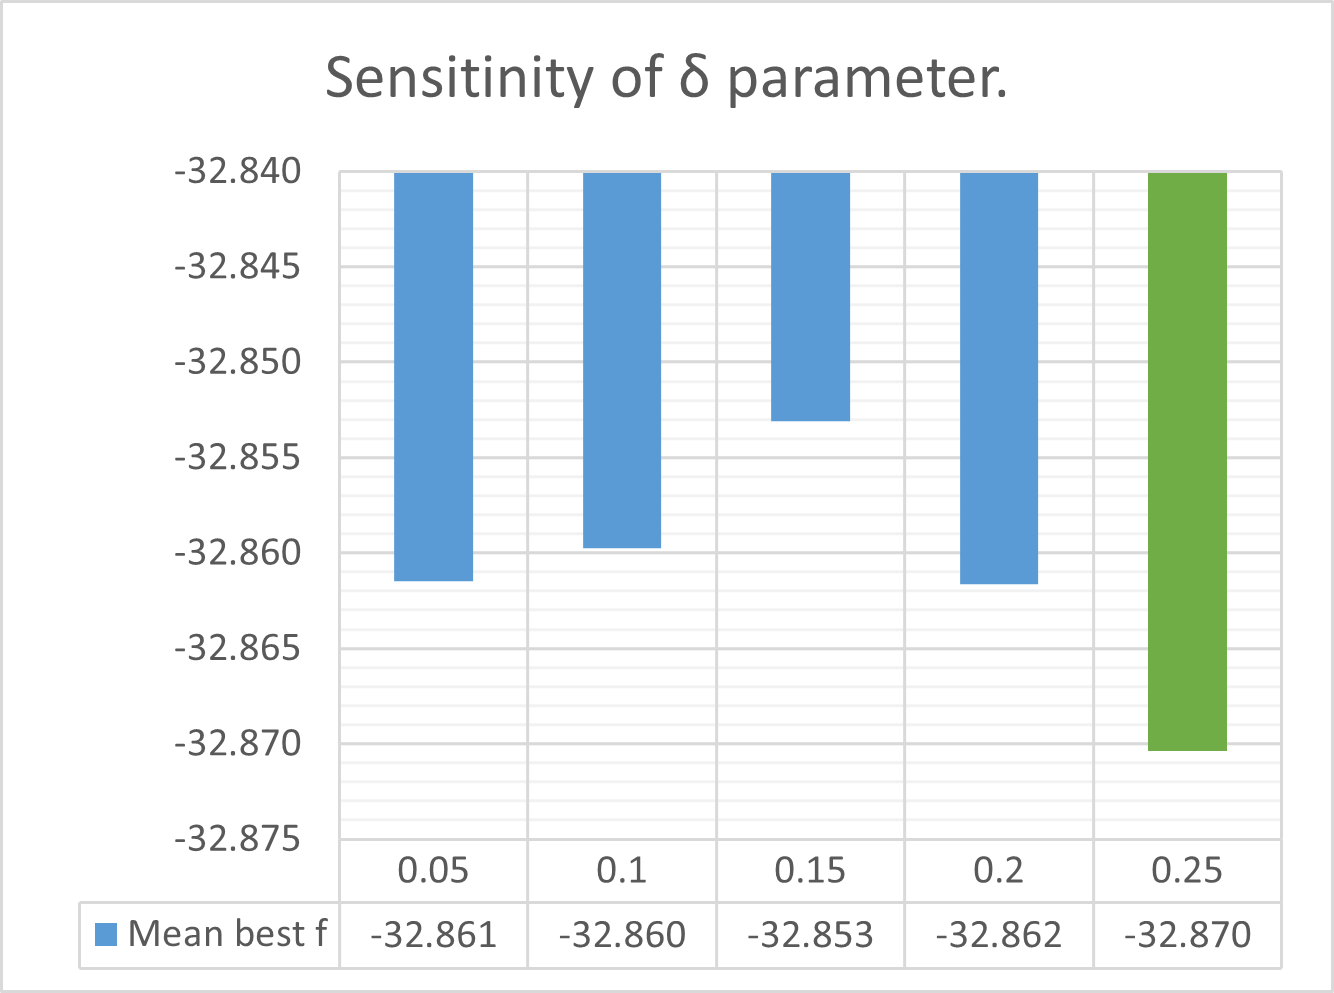
\includegraphics[scale=0.45]{tersoffc_d}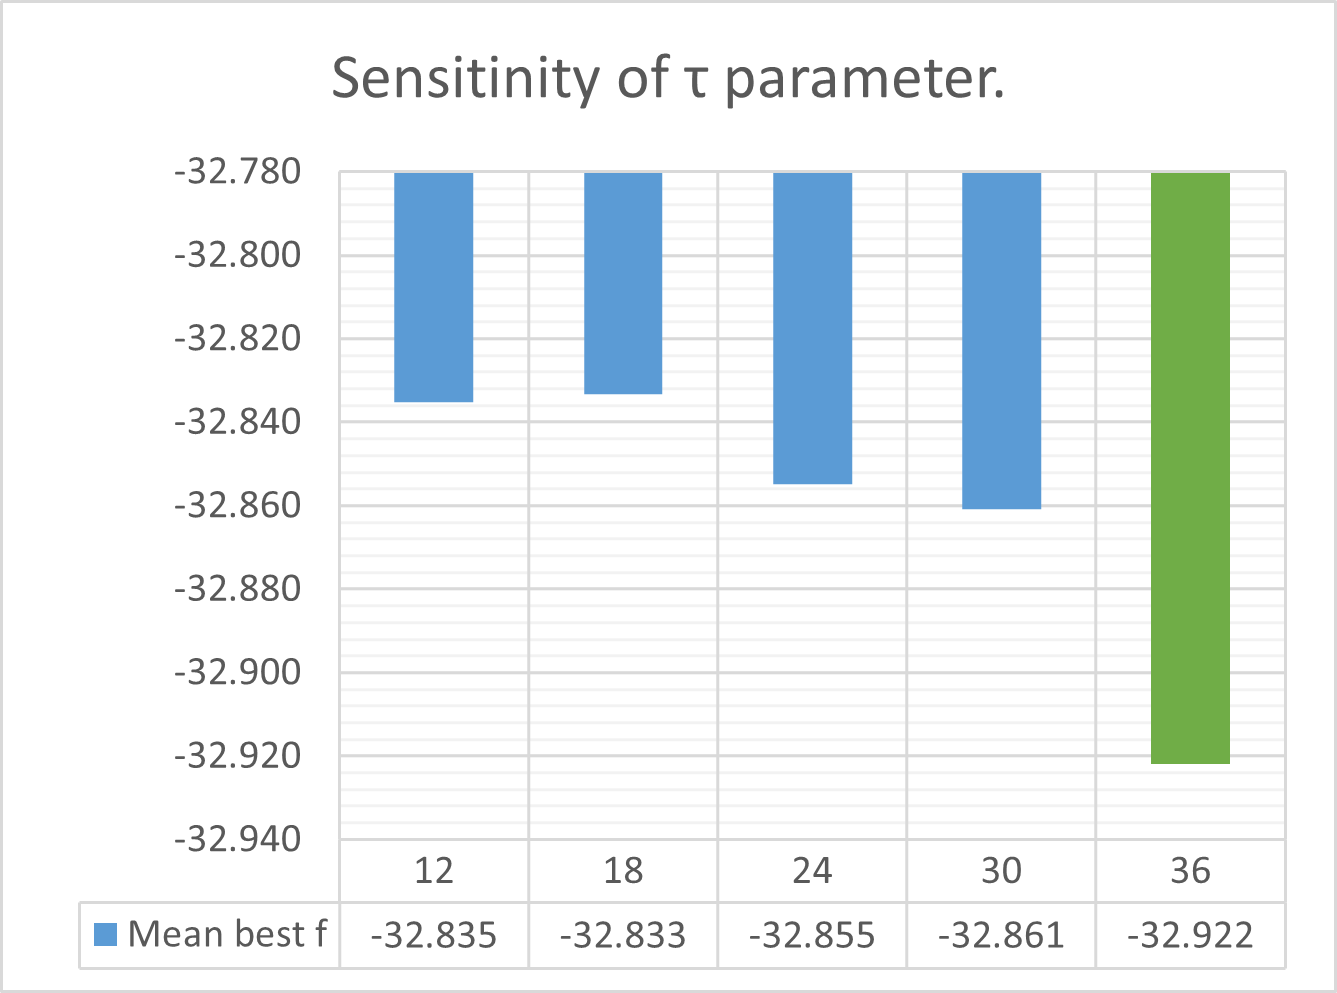
\includegraphics[scale=0.45]{tersoffc_t}
\par\end{centering}
\caption{Tersoffc problem.\label{fig:tersoffc}}
\end{figure}
\begin{figure}[H]
\begin{centering}
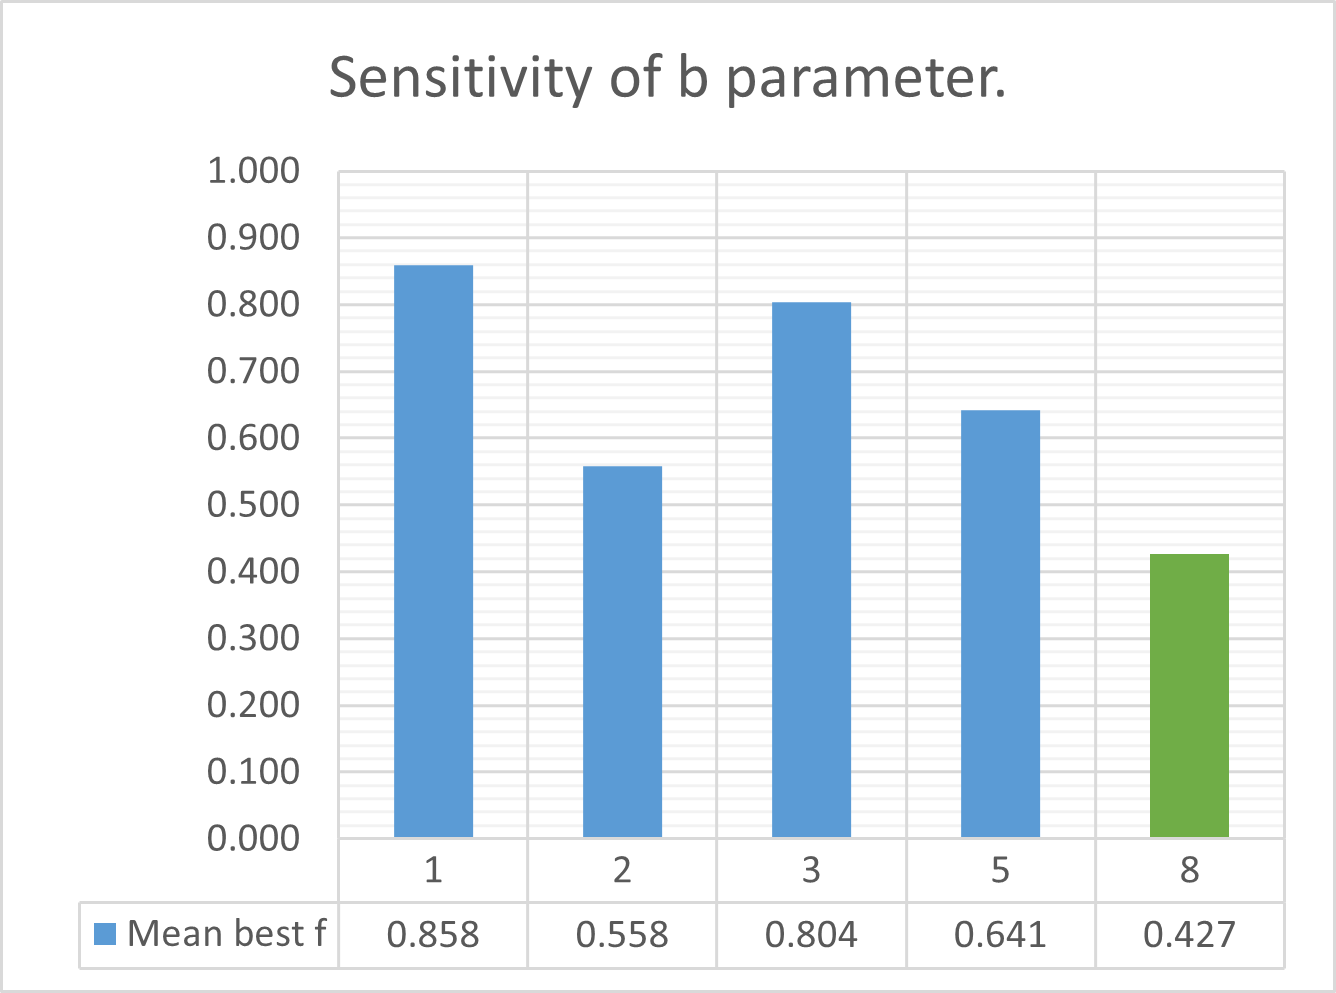
\includegraphics[scale=0.45]{weiresrass_b}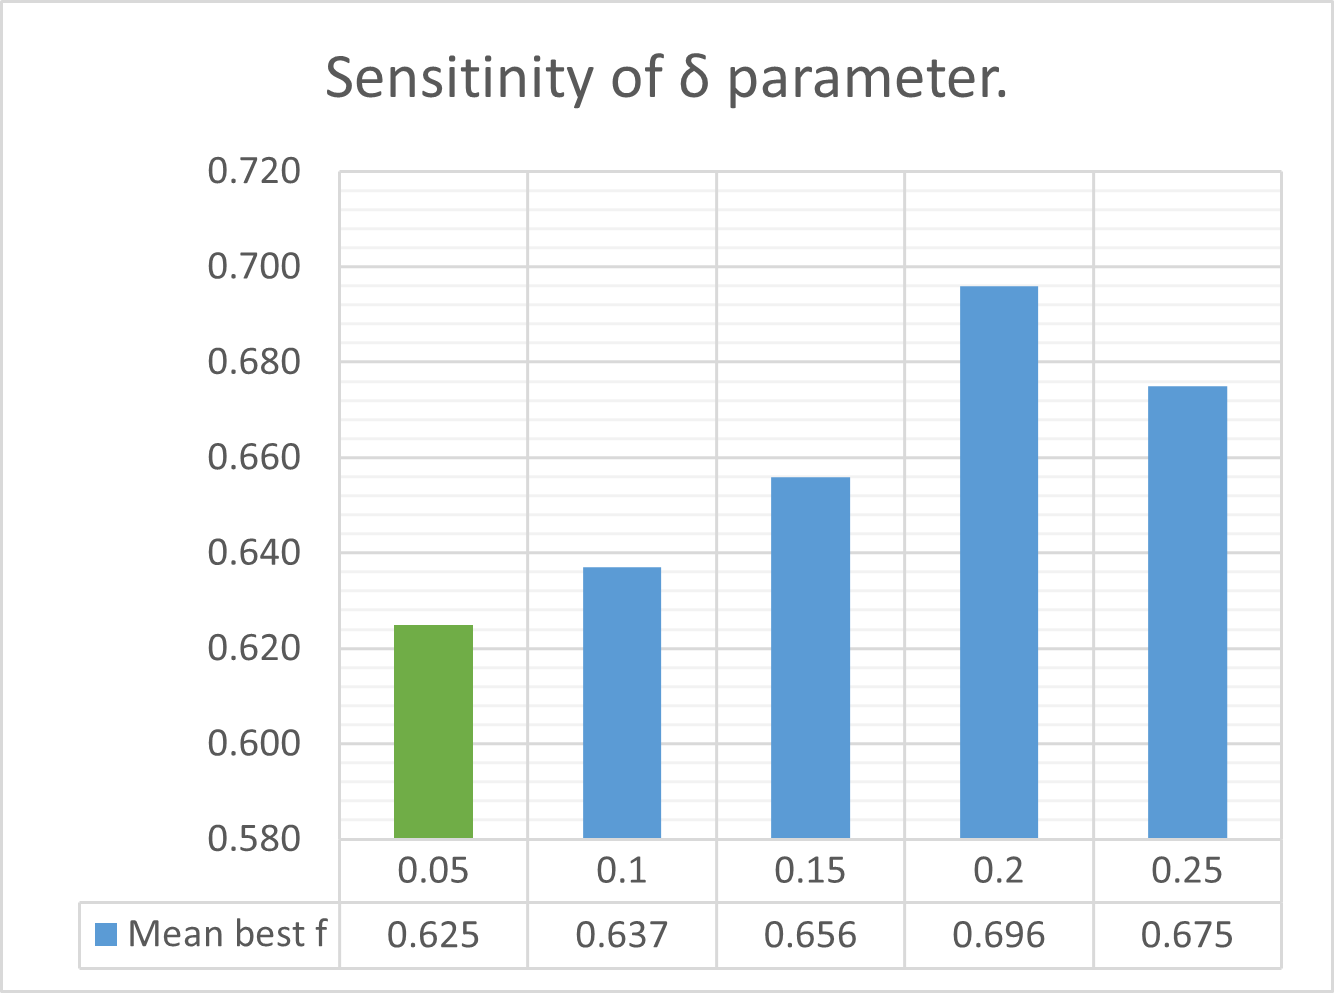
\includegraphics[scale=0.45]{weiresrass_d}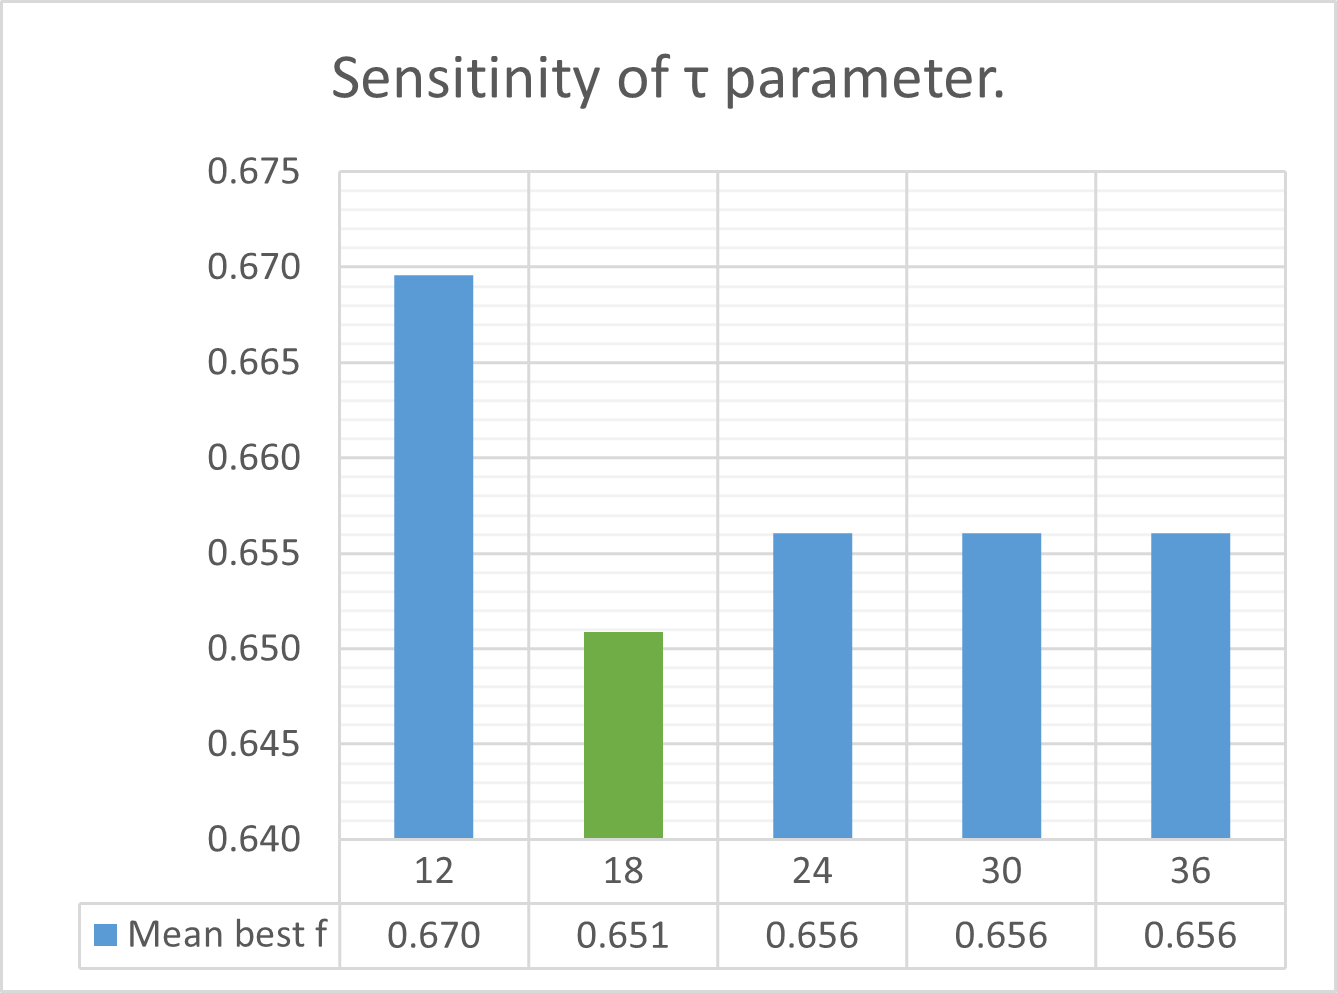
\includegraphics[scale=0.45]{weiresrass_t}
\par\end{centering}
\caption{Weiresrtrass problem. Dimension 50.\label{fig:weiresrtrass50}}
\end{figure}

The sensitivity results across the three benchmark problems reveal
a consistent pattern: the performance of ARQ2 is not critically dependent
on any of the three examined parameters, and the default configuration
used throughout the study remains competitive or optimal across all
tested settings. The bootstrap length b exhibits minimal influence
on tersoffc and moderate influence on weierstrass, where longer bootstrap
values tend to yield slightly better mean performance, while b=2 consistently
produces competitive results across all three problems. The reset
threshold $\delta$ shows the greatest variation on the high-dimensional
test2n problem, where larger values of $\delta$, corresponding to
more frequent credit resets, progressively improve mean performance,
suggesting that sustained branch competition is particularly beneficial
when the search space is large and the evaluation budget is relatively
tight. On tersoffc, however, $\delta$ produces negligible variation
across all tested levels, indicating that the scheduler behavior has
little influence on problems where the landscape structure itself
determines the difficulty. The stagnation trigger $\tau$ exhibits
moderate sensitivity on test2n, where values in the range $\tau$=12
to $\tau$=18 tend to produce better mean outcomes than larger values,
while on tersoffc and weierstrass the differences across all tested
values remain small. Taken together, these results support the conclusion
that ARQ2 maintains stable behavior over a reasonable range of parameter
values and that its performance advantage is not contingent on precise
parameter tuning. The observed variations are consistent with the
general expectation that high-dimensional problems are more sensitive
to scheduler and restart parameters, while lower-dimensional problems
with complex landscape structure are primarily governed by the search
dynamics themselves rather than by the specific control parameter
settings.

\subsection{Strengths and weaknesses of the proposed method\label{subsec:strengthsWeaknesses}}

The strengths and weaknesses of ARQ2 become clearer when the direct
ARQ2-versus-ARQ comparison is read together with the value-based and
ranking-based tables. The global picture remains favorable to the
proposed method. Table \ref{tab:finalR} places ARQ2 first overall
with a best total rank of 66, a mean total rank of 75, an overall
rank sum of 141, and an average rank of 1.9583. This result is important
because it is supported jointly by best-value and mean-value evidence
rather than by a single evaluation criterion. In aggregate terms,
ARQ2 therefore achieves the strongest overall balance between peak
solution quality and repeated-run robustness on the complete benchmark
suite. The overall first position of ARQ2 is determined by the total
rank sum rather than by the count of rank-1 placements. Although EA4Eig
records more rank-1 outcomes in Table \ref{tab:meanR}, its total
mean rank of 85 is substantially higher than that of ARQ2 at 75, indicating
that EA4Eig attains top positions on fewer problems while performing
less competitively on the remainder. ARQ2, by contrast, maintains
a more uniformly strong position across the full benchmark suite,
which is the criterion captured by the aggregate rank sum in Table
\ref{tab:finalR}.

A major strength of ARQ2 is its clear improvement over the original
ARQ, especially in average-case behavior. Table \ref{tab:arq2VSarq}
shows that, in terms of best values, ARQ2 performs better than ARQ
on 10 problems, matches it on 18, and is worse on 8. The corresponding
comparison in terms of mean values is substantially more favorable
to ARQ2, which improves upon ARQ on 21 problems, matches it on 11,
and is worse on only 4. The same general tendency appears in the variability
indicators, where ARQ2 attains lower standard deviation on 20 problems,
equal standard deviation on 11, and higher standard deviation on only
5. This pattern is consistent with the ranking tables, where the transition
from ARQ to ARQ2 improves the best total rank from 81 to 66 and, even
more importantly, improves the mean total rank from 145 to 75. The
proposed extension therefore appears to strengthen ARQ primarily at
the level of reliability, stability, and repeated-run competitiveness,
rather than only at the level of isolated favorable outcomes. The
cases where ARQ2 yields a worse best value than ARQ can be attributed
to the inherent cost of hybridization. By distributing evaluations
between two branches under the roulette scheduler, ARQ2 allocates
a fraction of its computational budget to the IDE branch, which may
divert search effort away from the most productive region on problems
where the ARQ search dynamic alone would have been sufficient. This
trade-off is the expected consequence of designing for robustness
across a heterogeneous benchmark suite rather than for peak performance
on any specific problem class.

Another important strength of ARQ2 is its positional consistency across
the full benchmark collection. In Table \ref{tab:bestR}, ARQ2 achieves
25 rank-1 placements and 29 top-three placements, which gives it the
lowest best-based total rank among all compared methods. In Table
\ref{tab:meanR}, it records 31 top-three placements and no placements
in the lower-performance tail of the ranking distribution, again yielding
the best total rank. This is a particularly strong feature of the
method: ARQ2 is not merely competitive because of a limited number
of exceptional runs, but because it remains close to the leading positions
over a large portion of the benchmark suite. The same conclusion is
supported by Tables \ref{tab:bestR} and \ref{tab:meanR}. ARQ2 reaches
the best recorded final value on 25 problems when ties are counted,
which is the highest count among all methods, while in mean-value
terms it remains among the strongest methods even though the competition
becomes more evenly distributed.

When the benchmark is viewed through its real-world and non-realworld
components, an additional strength of ARQ2 becomes visible. Over the
real-world subset introduced in Section \ref{sec:results}, ARQ2 obtains
the best aggregate behavior in both criteria, with a best-rank average
of 2.0417 and a mean-rank average of 1.9583. This is a meaningful
result because the practical relevance of the study depends heavily
on these application-oriented problems. At the same time, the non-realworld
subset reveals a more nuanced picture. ARQ2 remains the strongest
method in best-value terms on the classical benchmark functions, with
an average best rank of 1.4167, but it is slightly surpassed by EA4Eig
in mean-value terms, where ARQ2 attains an average mean rank of 2.3333
against 2.0833 for EA4Eig. This indicates that ARQ2 retains strong
peak performance on the synthetic part of the benchmark, while its
average behavior on that subset is not uniformly dominant against
the strongest competitor.

This last point leads directly to the main weaknesses of the proposed
method. The first weakness is that ARQ2 is not the per-problem leader
in mean-value behavior as often as its overall first position might
initially suggest. In Table \ref{tab:meanR}, EA4Eig records 19 rank-1
placements and JSO records 17, whereas ARQ2 records 15. The overall
advantage of ARQ2 therefore comes less from dominating every individual
problem and more from maintaining a more uniform competitive profile
across the suite. The second weakness is that a number of difficult
problems remain clearly challenging. In best-based ranking terms,
relatively weak placements are observed on tersoffb and vibratingplatform,
where ARQ2 receives rank 6, and on ded1, ded2, eld5, hydrothermal,
and rotatedrosenbrock, where it receives rank 4. In mean-based terms,
the most visible weakness appears on sinusoidal, where ARQ2 receives
rank 6, while eld4, hydrothermal, transmissionpricing, and rotatedrosenbrock
remain at rank 4. These cases indicate that ARQ2 still encounters
difficulties on selected high-dimensional engineering instances and
on some structurally demanding synthetic landscapes.

The comparison with the strongest competitors also remains instructive.
EA4Eig is the closest overall rival of ARQ2 and appears particularly
strong in mean-value performance on the non-realworld subset. JSO
remains highly competitive on selected problems and retains a large
number of rank-1 outcomes, especially in value-based comparisons.
MLSHADE-RL, although not first overall, also maintains consistently
strong aggregate positions. Against this backdrop, the advantage of
ARQ2 should not be interpreted as universal dominance, but as the
most favorable overall compromise among the compared methods. Its
central strength lies in combining strong best-case performance, strong
aggregate mean behavior, and a marked improvement over ARQ in repeated-run
reliability. Its central weakness is that this advantage is not uniform
across all problem classes, especially on some demanding real-world
scheduling and design problems and on a few difficult non-realworld
functions. Even so, the evidence of the tables supports the conclusion
that ARQ2 offers the most balanced general-purpose performance profile
in the present study.

\section{Conclusions\label{sec:conclusions}}

This study presented ARQ2 and evaluated its performance on a heterogeneous
benchmark suite of 36 continuous optimization problems, comprising
both real-world and classical instances. The experimental results
confirm that ARQ2 achieves the strongest overall aggregate performance
among the ten compared methods, attaining the lowest total rank sum
of 141 and an average rank of 1.958 across best-value and mean-value
criteria jointly. Compared to its predecessor ARQ, the proposed extension
improves mean-value performance on 21 out of 36 problems and attains
lower solution variability on 20 problems, demonstrating that the
primary contribution of ARQ2 lies in strengthening repeated-run reliability
rather than producing isolated favorable outcomes.

At the same time, the results make clear that ARQ2 is not universally
superior across all problem classes, and that strong competitors such
as EA4Eig, MLSHADE-RL, and JSO remain highly competitive on selected
problems. The present findings should therefore be interpreted as
evidence of strong general competitiveness and improved robustness,
while also identifying specific problem classes where further refinement
remains warranted. In this sense, the current study establishes a
solid basis for the next stage of methodological development of the
ARQ design line.

\appendixtitles{no}

\begin{adjustwidth}{-\extralength}{0cm}{}

\begin{thebibliography}{999}
\bibitem[(2013)]{Rios}Rios, L. M., \& Sahinidis, N. V. (2013). Derivative-free
optimization: A review of algorithms and comparison of software implementations.
Journal of Global Optimization, 56(3), 1247-1293. https://doi.org/10.1007/s10898-012-9951-y

\bibitem[(2002)]{Coello}Coello Coello, C. A. (2002). Theoretical
and numerical constraint-handling techniques used with evolutionary
algorithms: A survey of the state of the art. Computer Methods in
Applied Mechanics and Engineering, 191(11-12), 1245-1287. https://doi.org/10.1016/S0045-7825(01)00323-1

\bibitem[(1983)]{Kirkpatrick}Kirkpatrick, S., Gelatt, C. D., Jr.,
\& Vecchi, M. P. (1983). Optimization by simulated annealing. Science,
220(4598), 671-680. https://doi.org/10.1126/science.220.4598.671

\bibitem[(1995)]{Kennedy}Kennedy, J., \& Eberhart, R. (1995). Particle
swarm optimization. In Proceedings of ICNN'95-International Conference
on Neural Networks (Vol. 4, pp. 1942-1948). IEEE. https://doi.org/10.1109/ICNN.1995.488968

\bibitem[(2001)]{Hansen}Hansen, N., \& Ostermeier, A. (2001). Completely
derandomized self-adaptation in evolution strategies. Evolutionary
Computation, 9(2), 159-195. https://doi.org/10.1162/106365601750190398

\bibitem[(1996)]{Dorigo}Dorigo, M., Maniezzo, V., \& Colorni, A.
(1996). Ant system: Optimization by a colony of cooperating agents.
IEEE Transactions on Systems, Man, and Cybernetics-Part B: Cybernetics,
26(1), 29-41. https://doi.org/10.1109/3477.484436

\bibitem[(1989)]{Glover}Glover, F. (1989). Tabu search-Part I. ORSA
Journal on Computing, 1(3), 190-206. https://doi.org/10.1287/ijoc.1.3.190

\bibitem[(2003)]{Glover2}Glover, F., Laguna, M., \& Martí, R. (2003).
Scatter search. In A. Ghosh \& S. Tsutsui (Eds.), Advances in evolutionary
computing (pp. 519-537). Springer. https://doi.org/10.1007/978-3-642-18965-4\_20

\bibitem[(2001)]{Geem}Geem, Z. W., Kim, J. H., \& Loganathan, G.
V. (2001). A new heuristic optimization algorithm: Harmony search.
Simulation, 76(2), 60-68. https://doi.org/10.1177/003754970107600201

\bibitem[(2007)]{Karaboga}{[}Karaboga, D., \& Basturk, B. (2007).
A powerful and efficient algorithm for numerical function optimization:
Artificial bee colony (ABC) algorithm. Journal of Global Optimization,
39(3), 459-471. https://doi.org/10.1007/s10898-007-9149-x

\bibitem[(2010)]{Yang}Yang, X.-S. (2010). Firefly algorithm, stochastic
test functions and design optimisation. International Journal of Bio-Inspired
Computation, 2(2), 78-84. https://doi.org/10.1504/IJBIC.2010.032124

\bibitem[(2009)]{Yang2}Yang, X.-S., \& Deb, S. (2009). Cuckoo search
via Lévy flights. In 2009 World Congress on Nature \& Biologically
Inspired Computing (NaBIC) (pp. 210-214). IEEE. https://doi.org/10.1109/NABIC.2009.5393690

\bibitem[(2010)]{Yang3}Yang, X.-S. (2010). A new metaheuristic bat-inspired
algorithm. In Nature inspired cooperative strategies for optimization
(NICSO 2010) (pp. 65-74). Springer. https://doi.org/10.1007/978-3-642-12538-6\_6

\bibitem[(2010)]{Rao}Rao, R. V., Savsani, V. J., \& Vakharia, D.
P. (2011). Teaching-learning-based optimization: A novel method for
constrained mechanical design optimization problems. Computer-Aided
Design, 43(3), 303-315. https://doi.org/10.1016/j.cad.2010.12.015

\bibitem[(2009)]{Rashedi}Rashedi, E., Nezamabadi-Pour, H., \& Saryazdi,
S. (2009). GSA: A gravitational search algorithm. Information Sciences,
179(13), 2232-2248. https://doi.org/10.1016/j.ins.2009.03.004

\bibitem[(2014)]{Mirjalili}Mirjalili, S., Mirjalili, S. M., \& Lewis,
A. (2014). Grey wolf optimizer. Advances in Engineering Software,
69, 46-61. https://doi.org/10.1016/j.advengsoft.2013.12.007

\bibitem[(2016)]{Mirjalili2}Mirjalili, S., \& Lewis, A. (2016). The
whale optimization algorithm. Advances in Engineering Software, 95,
51-67. https://doi.org/10.1016/j.advengsoft.2016.01.008

\bibitem[(2008)]{Simon}Simon, D. (2008). Biogeography-based optimization.
IEEE Transactions on Evolutionary Computation, 12(6), 702-713. https://doi.org/10.1109/TEVC.2008.919004

\bibitem[(2006)]{Mehrabian}Mehrabian, A. R., \& Lucas, C. (2006).
A novel numerical optimization algorithm inspired from weed colonization.
Ecological Informatics, 1(4), 355-366. https://doi.org/10.1016/j.ecoinf.2006.07.003

\bibitem[(2003)]{Eusuff}Eusuff, M. M., \& Lansey, K. E. (2003). Optimization
of water distribution network design using the shuffled frog leaping
algorithm. Journal of Water Resources Planning and Management, 129(3),
210-225. https://doi.org/10.1061/(ASCE)0733-9496(2003)129:3(210)

\bibitem[(2005)]{Krasnogor}Krasnogor, N., \& Smith, J. (2005). A
tutorial for competent memetic algorithms: Model, taxonomy, and design
issues. IEEE Transactions on Evolutionary Computation, 9(5), 474-488.
https://doi.org/10.1109/TEVC.2005.850260

\bibitem[(2002)]{Larra=0000F1aga}Larrañaga, P., \& Lozano, J. A.
(Eds.). (2002). Estimation of distribution algorithms: A new tool
for evolutionary computation. Springer. https://doi.org/10.1007/978-1-4615-1539-5

\bibitem[(1997)]{Storn}Storn, R., \& Price, K. (1997). Differential
evolution: A simple and efficient heuristic for global optimization
over continuous spaces. Journal of Global Optimization, 11(4), 341-359.
https://doi.org/10.1023/A:1008202821328

\bibitem[(2022)]{Ahmad}Ahmad, M. F., Isa, N. A. M., Lim, W. H., \&
Ang, K. M. (2022). Differential evolution: A recent review based on
state-of-the-art works. Alexandria Engineering Journal, 61(5), 3831-3872.
https://doi.org/10.1016/j.aej.2021.09.013

\bibitem[(2006)]{Brest}Brest, J., Greiner, S., Bošković, B., Mernik,
M., \& Žumer, V. (2006). Self-adapting control parameters in differential
evolution: A comparative study on numerical benchmark problems. IEEE
Transactions on Evolutionary Computation, 10(6), 646-657. https://doi.org/10.1109/TEVC.2006.872133

\bibitem[(2009)]{Qin}Qin, A. K., Huang, V. L., \& Suganthan, P. N.
(2009). Differential evolution algorithm with strategy adaptation
for global numerical optimization. IEEE Transactions on Evolutionary
Computation, 13(2), 398-417. https://doi.org/10.1109/TEVC.2008.927706

\bibitem[(2009)]{Zhang}Zhang, J., \& Sanderson, A. C. (2009). JADE:
Adaptive differential evolution with optional external archive. IEEE
Transactions on Evolutionary Computation, 13(5), 945-958. https://doi.org/10.1109/TEVC.2009.2014613

\bibitem[(2011)]{Wang}Wang, Y., Cai, Z., \& Zhang, Q. (2011). Differential
evolution with composite trial vector generation strategies and control
parameters. IEEE Transactions on Evolutionary Computation, 15(1),
55-66. https://doi.org/10.1109/TEVC.2010.2087271

\bibitem[(2013)]{Wang2}Tanabe, R., \& Fukunaga, A. (2013). Success-history
based parameter adaptation for differential evolution. In 2013 IEEE
Congress on Evolutionary Computation (CEC) (pp. 71-78). IEEE. https://doi.org/10.1109/CEC.2013.6557555

\bibitem[(2014)]{Tanabe}Tanabe, R., \& Fukunaga, A. S. (2014). Improving
the search performance of SHADE using linear population size reduction.
In 2014 IEEE Congress on Evolutionary Computation (CEC) (pp. 1658-1665).
IEEE. https://doi.org/10.1109/CEC.2014.6900380

\bibitem[(2011)]{Das}Das, S., \& Suganthan, P. N. (2011). Differential
evolution: A survey of the state-of-the-art. IEEE Transactions on
Evolutionary Computation, 15(1), 4-31. https://doi.org/10.1109/TEVC.2010.2059031

\bibitem[(2025)]{Charilogis}Charilogis, V., Tsoulos, I. G., Gianni,
A. M., \& Tsalikakis, D. (2025). ARQ: A cohesive optimization design
for stable performance on noisy landscapes. Applied Sciences, 15(22),
12180. doi:10.3390/app152212180.

\bibitem[(2022)]{Bujok}Bujok, P., \& Kolenovský, P. (2022). Eigen
crossover in cooperative model of evolutionary algorithms applied
to CEC 2022 single objective numerical optimisation. In 2022 IEEE
Congress on Evolutionary Computation (CEC) (pp. 1-8). doi:10.1109/CEC55065.2022.9870433.

\bibitem[(2017)]{Brest2}Brest, J., Maučec, M. S., \& Bošković, B.
(2017). Single objective real-parameter optimization: Algorithm jSO.
In 2017 IEEE Congress on Evolutionary Computation (CEC) (pp. 1311-1318).
doi:10.1109/CEC.2017.7969456.

\bibitem[(2006)]{Brest3}Brest, J., Greiner, S., Bošković, B., Mernik,
M., \& Žumer, V. (2006). Self-adapting control parameters in differential
evolution: A comparative study on numerical benchmark problems. IEEE
Transactions on Evolutionary Computation, 10(6), 646-657. doi:10.1109/TEVC.2006.872133.

\bibitem[(2024)]{Chauhan}Chauhan, D., Trivedi, A., \& Shivani. (2024).
A multi-operator ensemble LSHADE with restart and local search mechanisms
for single-objective optimization. arXiv. doi:10.48550/arXiv.2409.15994.

\bibitem[(2006)]{Liang}Liang, J. J., Qin, A. K., Suganthan, P. N.,
\& Baskar, S. (2006). Comprehensive learning particle swarm optimizer
for global optimization of multimodal functions. IEEE Transactions
on Evolutionary Computation, 10(3), 281-295. doi:10.1109/TEVC.2005.857610.

\bibitem[(2025)]{Charilogis2}Charilogis, V., Tsoulos, I. G., \& Gianni,
A. M. (2025). TRIDENT-DE: Triple-operator differential evolution with
adaptive restarts and greedy refinement. Future Internet, 17(11),
488. doi:10.3390/fi17110488.

\bibitem[(2024)]{Trivedi}Trivedi, A., \& Chauhan, D. (2024). UDE-III:
An enhanced unified differential evolution algorithm for constrained
optimization problems. arXiv. doi:10.48550/arXiv.2410.03992.

\bibitem[(2009)]{Qin2}Qin, A. K., Huang, V. L., \& Suganthan, P.
N. (2009). Differential evolution algorithm with strategy adaptation
for global numerical optimization. IEEE Transactions on Evolutionary
Computation, 13(2), 398-417. doi:10.1109/TEVC.2008.927706.

\bibitem[(2015)]{Al-Roomi}Al-Roomi, A. R. (2015). IEEE Congresses
on Evolutionary Computation repository. Dalhousie University, Electrical
and Computer Engineering.

\bibitem[(2022)]{Biedrzycki}Biedrzycki, R. (2025). Analysis and simplification
of the winner of the CEC 2022 optimization competition on single objective
bound constrained search. Evolutionary Computation, 1-19. doi:10.1162/evco\_a\_00327.

\bibitem[(2010)]{antennaarrayantennaula}Chowdhury, A., Giri, R.,
Ghosh, A., Das, S., Abraham, A., \& Snášel, V. (2010). Linear antenna
array synthesis using fitness-adaptive differential evolution algorithm.
In 2010 IEEE Congress on Evolutionary Computation (pp. 1-8). IEEE.
https://doi.org/10.1109/CEC.2010.5586518

\bibitem[(1976)]{bifunctionalcatalyst1}Hofer, E. P. (1976). Optimization
of bifunctional catalysts in tubular reactors. Journal of Optimization
Theory and Applications, 18(3), 379-393. https://doi.org/10.1007/BF00933819

\bibitem[(1992)]{bifunctionalcatalyst2}Luus, R., Dittrich, J., \&
Keil, F. J. (1992). Multiplicity of solutions in the optimization
of a bifunctional catalyst blend in a tubular reactor. The Canadian
Journal of Chemical Engineering, 70(4), 780-785. https://doi.org/10.1002/cjce.5450700423

\bibitem[(1994)]{bifunctionalcatalyst3}Luus, R., \& Bojkov, B. (1994).
Global optimization of the bifunctional catalyst problem. The Canadian
Journal of Chemical Engineering, 72(1), 160-163. https://doi.org/10.1002/cjce.5450720125

\bibitem[(2011)]{cec2011}Elsayed, S. M., Sarker, R. A., \& Essam,
D. L. (2011). Differential evolution with multiple strategies for
solving CEC2011 real-world numerical optimization problems. In 2011
IEEE Congress on Evolutionary Computation (pp. 1041-1048). IEEE. https://doi.org/10.1109/CEC.2011.5949732

\bibitem[(2011)]{ik6dof}Aghajarian, M., \& Kiani, K. (2011). Inverse
kinematics solution of PUMA 560 robot arm using ANFIS. In 2011 8th
International Conference on Ubiquitous Robots and Ambient Intelligence
(pp. 574-578). IEEE. https://doi.org/10.1109/URAI.2011.6145885

\bibitem[(2021)]{messengertandem}Schlueter, M., Neshat, M., Wahib,
M., Munetomo, M., \& Wagner, M. (2021). GTOPX space mission benchmarks.
SoftwareX, 14, 100666. https://doi.org/10.1016/j.softx.2021.100666

\bibitem[(2009)]{polyphase}He, H., Stoica, P., \& Li, J. (2009).
Designing unimodular sequence sets with good correlations---Including
an application to MIMO radar. IEEE Transactions on Signal Processing,
57(11), 4391-4405. https://doi.org/10.1109/TSP.2009.2025108

\bibitem[(1924)]{potential}Jones, J. E. (1924). On the determination
of molecular fields. II. From the equation of state of a gas. Proceedings
of the Royal Society A: Mathematical, Physical and Engineering Sciences,
106(738), 463-477. https://doi.org/10.1098/rspa.1924.0082

\bibitem[(1952)]{portfoliomv}Markowitz, H. (1952). Portfolio selection.
The Journal of Finance, 7(1), 77-91. https://doi.org/10.1111/j.1540-6261.1952.tb01525.x

\bibitem[(1988)]{tersoffb}Tersoff, J. (1988). New empirical approach
for the structure and energy of covalent systems. Physical Review
B, 37(12), 6991-7000. https://doi.org/10.1103/PhysRevB.37.6991

\bibitem[(1989)]{tersoffc}Tersoff, J. (1989). Modeling solid-state
chemistry: Interatomic potentials for multicomponent systems. Physical
Review B, 39(8), 5566-5568. https://doi.org/10.1103/PhysRevB.39.5566

\bibitem[(1970)]{transmissionpricing1}Garver, L. L. (1970). Transmission
network estimation using linear programming. IEEE Transactions on
Power Apparatus and Systems, PAS-89(7), 1688-1697. https://doi.org/10.1109/TPAS.1970.292825

\bibitem[(1988)]{transmissionpricing2}Schweppe, F. C., Caramanis,
M. C., Tabors, R. D., \& Bohn, R. E. (1988). Spot pricing of electricity.
Springer. https://doi.org/10.1007/978-1-4613-1683-1

\bibitem[(2024)]{wirelesscoverage}Calles-Esteban, F., Olmedo, A.
A., Hellín, C. J., Valledor, A., Gómez, J., \& Tayebi, A. (2024).
Optimizing antenna positioning for enhanced wireless coverage: A genetic
algorithm approach. Sensors, 24(7), 2165. https://doi.org/10.3390/s24072165

\bibitem[(2020)]{Varelas}Varelas, K., Ait El Hara, O., Brockhoff,
D., Hansen, N., Nguyen, D. M., Tušar, T., \& Auger, A. (2020). Benchmarking
large-scale continuous optimizers: The bbob-largescale testbed, a
COCO software guide and beyond. Applied Soft Computing, 97, 106737.
https://doi.org/10.1016/j.asoc.2020.106737

\bibitem[(2013)]{Jamil}Jamil, M., \& Yang, X.-S. (2013). A literature
survey of benchmark functions for global optimisation problems. International
Journal of Mathematical Modelling and Numerical Optimisation, 4(2),
150-194. https://doi.org/10.1504/IJMMNO.2013.055204

\bibitem[(2005)]{Ali}Ali, M. M., Khompatraporn, C., \& Zabinsky,
Z. B. (2005). A numerical evaluation of several stochastic algorithms
on selected continuous global optimization test problems. Journal
of Global Optimization, 31(4), 635-672. https://doi.org/10.1007/s10898-004-9972-2 

\end{thebibliography}

\end{adjustwidth}{}
\end{document}
